
%\vspace{-0.05in}
\section{Markov-chain Monte Carlo Estimators for Score Climbing}
\vspace{-0.05in}
\subsection{Overview of The Estimators}\label{section:overview}
%

% Second version of table, with booktabs.
%\begin{table}
%\centering
\caption{Computational Costs of MCSA Schemes}\label{table:cost}
\setlength{\tabcolsep}{0.5pt}
  \begin{threeparttable}
\begin{tabular}{lccccc}\toprule
& \multicolumn{3}{c}{\footnotesize Kernel Application} & \multicolumn{2}{c}{\footnotesize Gradient Estimation} \\
\cmidrule(lr){2-4}\cmidrule(lr){5-6}
  & {\footnotesize\(p\left( \vz, \vx \right)\)}
  & {\footnotesize\(q\left(\vz; \vlambda\right)\)}
  & {\footnotesize\(q\left(\vz; \vlambda\right)\)}
  & {\footnotesize\(p\left( \vz, \vx \right)\)}
  & {\footnotesize\( q\left(\vz; \vlambda\right)\)}
  \\
  & {\footnotesize\# Eval.  }
  & {\footnotesize\# Eval.  }
  & {\footnotesize\# Samples}
  & {\footnotesize\# Grad.  }
  & {\footnotesize\# Grad.  }
%
\\\midrule
%
{\footnotesize
ELBO
}
& \(0\)
& \(0\)
& \(N\)
& \(N\)
& \(N\)
\\\arrayrulecolor{black!30}\midrule
%
{\footnotesize
MSC
}
& \(N-1\)
& \(N\)
& \(N-1\)
& \(0\)
& \(1\)\tnote{1}\;\;{\footnotesize or}\;\(N\)\tnote{2}
\\
%
{\footnotesize
JSA
}
& \(N\)
& \(N+1\)
& \(N\)
& \(0\)
& \(N\)
\\
%
{\footnotesize
\textit{pMCSA}
}
& \(N\)
& \(2 \, N\)
& \(N\)
& \(0\)
& \(N\)
\\\bottomrule
\end{tabular}
  \begin{tablenotes}
    \item[*]{\footnotesize We assume that the parameters are cached as much as possible}.
    \item[1]{\footnotesize Vanilla CIS kernel}.
    \item[2]{\footnotesize Rao-Blackwellized CIS kernel}.
  \end{tablenotes}
  \end{threeparttable}
%\end{table}


\begin{figure*}
  \vspace{-0.5in}
    \centering
    \begin{subfigure}[b]{0.25\textwidth}
        \centering
        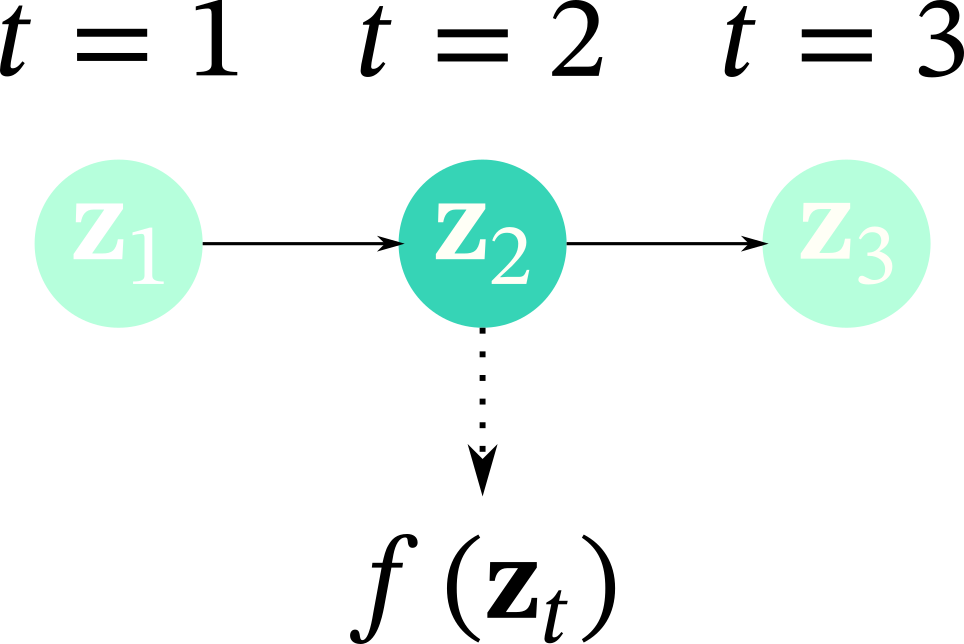
\includegraphics[scale=0.25]{figures/diagram_1.png}
        \caption{Single State Estimator}\label{fig:single}
    \end{subfigure}
    \begin{subfigure}[b]{0.35\textwidth}
        \centering
        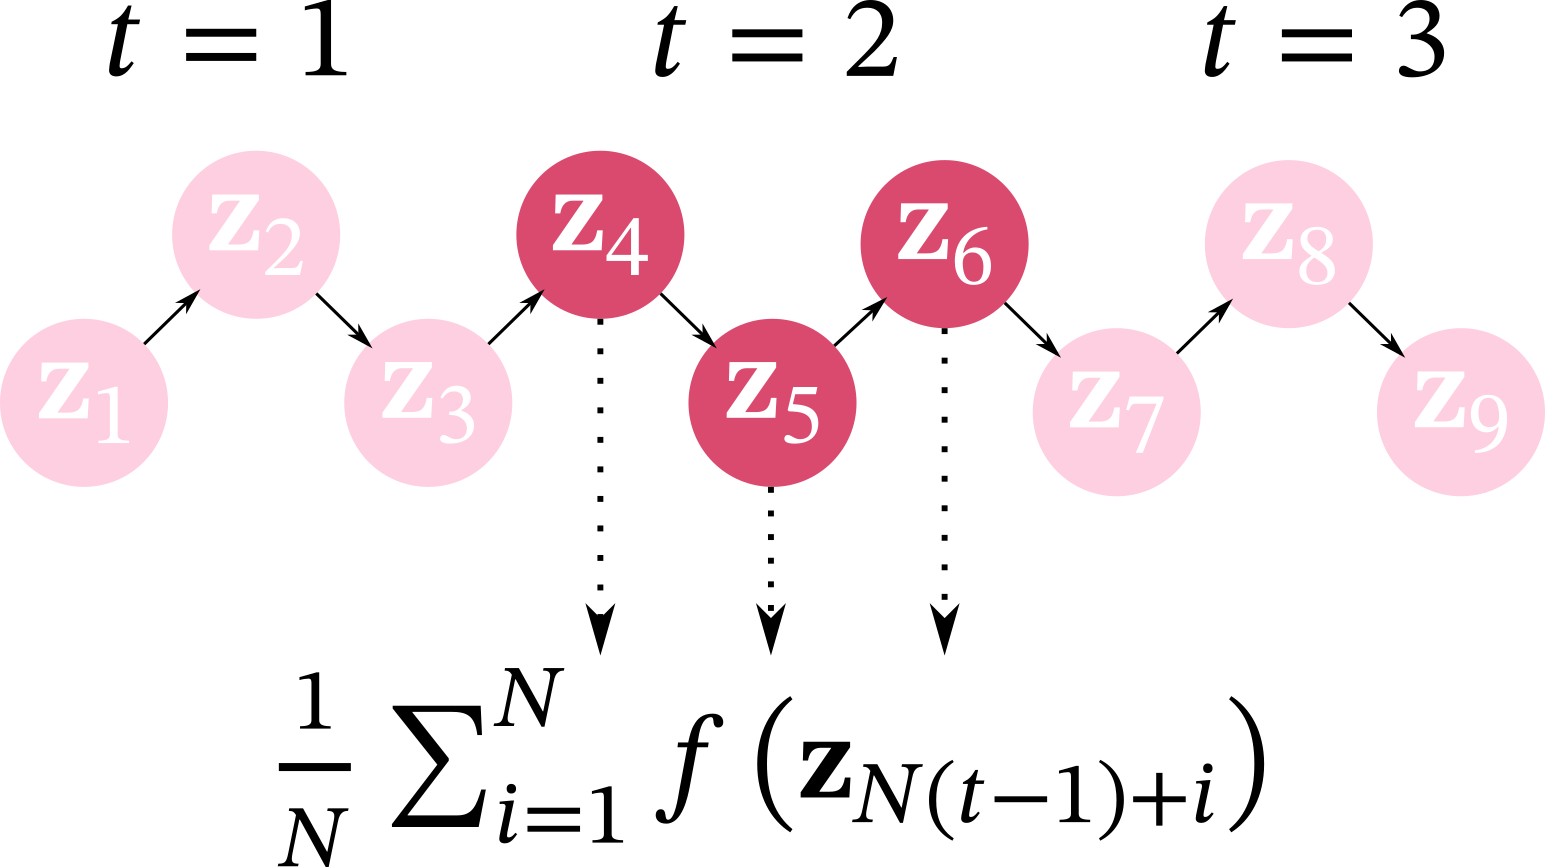
\includegraphics[scale=0.25]{figures/diagram_2.png}
        \caption{Sequential State Estimator}\label{fig:seq}
    \end{subfigure}
    \begin{subfigure}[b]{0.3\textwidth}
        \centering
        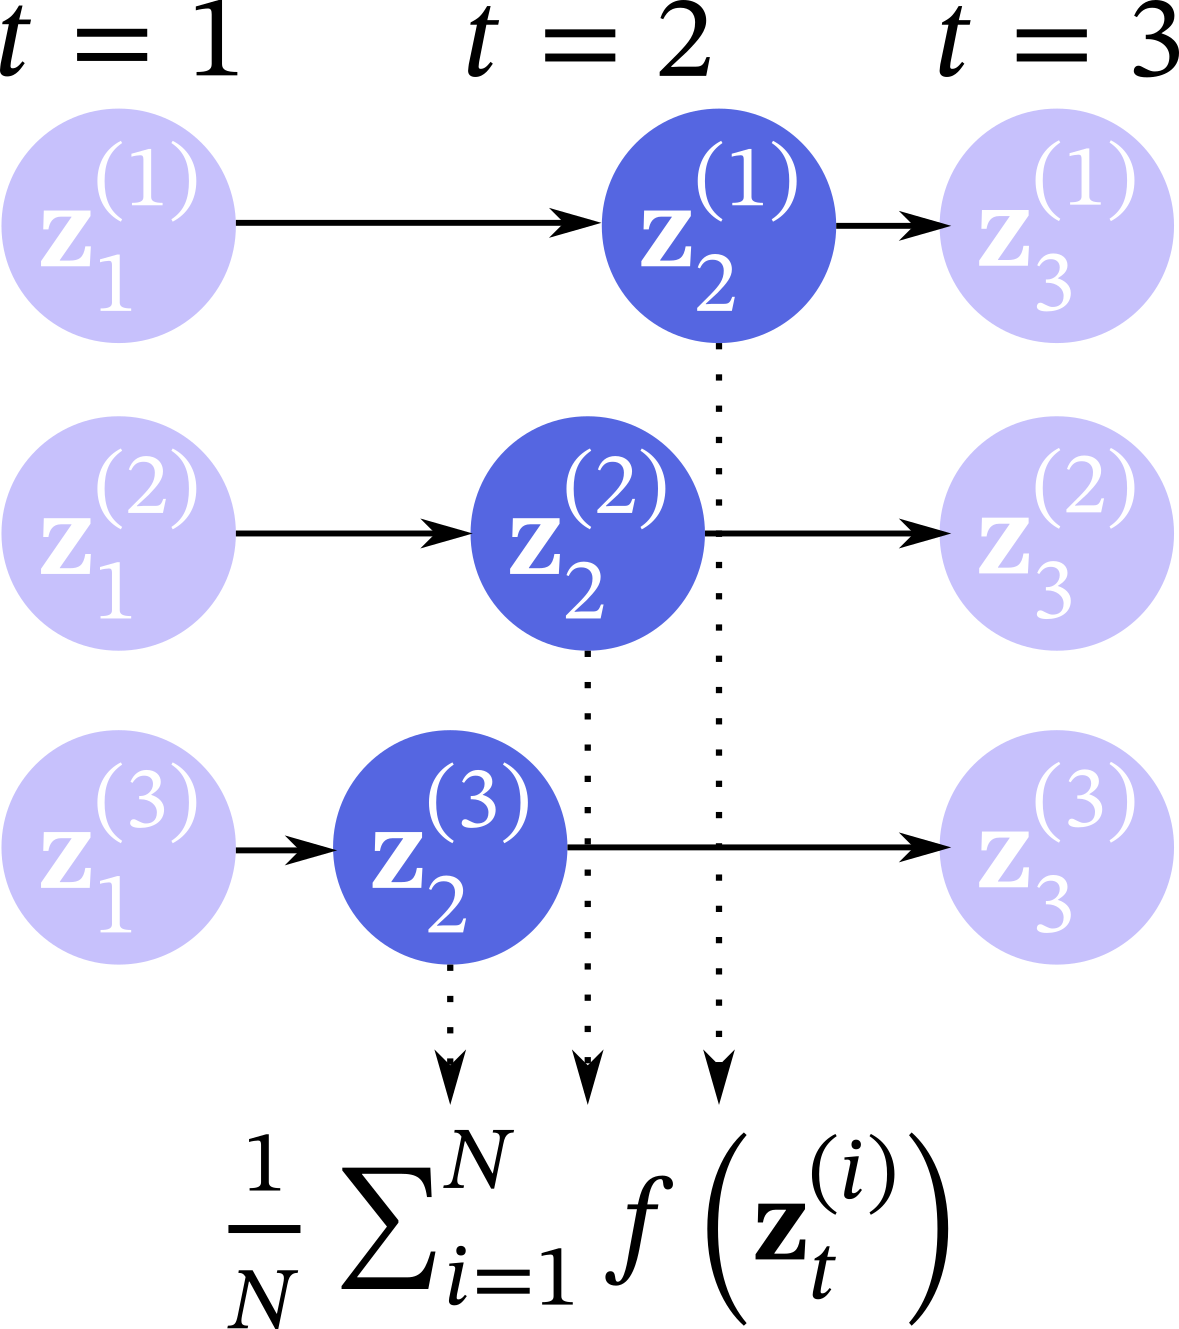
\includegraphics[scale=0.25]{figures/diagram_3.png}
        \caption{Parallel State Estimator (proposed)}\label{fig:par}
    \end{subfigure}
    \caption{Visualization of the three different ways to utilize MCMC for score climbing VI.
      The index \(t\) denotes the SGD iteration.
      The dark circles represent the MCMC samples used for estimating the score gradient at \(t=2\).
    }\label{fig:overview}
  \vspace{-0.1in}
\end{figure*}
%
\vspace{-0.05in}
\paragraph{Score Climbing with MCMC}
Recently,~\citet{NEURIPS2020_b2070693} and~\citet{pmlr-v124-ou20a} proposed two similar but independent score climbing method that minimize the inclusive KL with SGD.
Both methods estimate the score function gradient by operating a Markov-chain in parallel with the VI optimization sequence.
They notably use MCMC kernels that can effectively utilize the variational approximation \(q_{\vlambda_t}(\vz)\).
Because of this, both methods are computationally more efficient than previous VI approaches~\citep{pmlr-v97-ruiz19a, pmlr-v70-hoffman17a} that used expensive MCMC kernels such as Hamiltonian Monte Carlo.

\vspace{-0.05in}
\paragraph{Single State Estimator}
In Markovian score climbing (MSC),~\citet{NEURIPS2020_b2070693} estimate the score gradient by performing an MCMC transition and estimate the score function gradient as
\vspace{-0.05in}
\begin{align*}
  &\vz_t \sim K_{\vlambda_{t-1}}\left(\vz_{t-1}, \cdot \right),
  &\vg_{\text{single-CIS}}(\vlambda) = \vs\,(\vlambda; \vz_t),
\end{align*}
where \(K_{\vlambda_{t-1}}\left(\vz_{t-1}, \cdot\right)\) is a MCMC kernel leaving \(p\,(\vz\mid\vx)\) invariant and \(g_{\text{single}}\left(\vlambda\right)\) denotes the score estimator.
For the MCMC kernel, they propose to use what they call the conditional importance sampling (CIS, previously called iterated sampling importance resampling by~\citet{andrieu_uniform_2018}).
Since the estimator uses \textit{a single state} created by the CIS kernel, we call it the single state estimator with the CIS kernel (\textbf{single-CIS}).
The CIS kernel internally uses \(N\) samples from the \(q_{\vlambda_{t-1}}(\vz)\), hence the dependence on \(\vlambda_{t-1}\).
When compared to MCMC kernels that only use a single sample from \(q_{\vlambda_{t-1}}(\vz)\), it is \(N\) times more expensive, but hopefully, statistically superior.

\vspace{-0.08in}
\paragraph{Sequential State Estimator}
On the other hand, at each SGD iteration \(t\),~\citet{pmlr-v124-ou20a} perform \(N\) sequential Markov-chain transitions and use the average of the intermediate states for estimation.
That is, for the transition number \(n \in \{1, \ldots, N\}\),
\vspace{-0.05in}
\begin{align*}
  &\vz_{T+i} \sim K_{\vlambda_{t-1}}^i\left(\vz_{T}, \cdot \right),
  &\vg_{\text{seq.-IMH}}(\vlambda) = \frac{1}{N} \sum_{n=1}^N \vs\,(\vlambda; \vz_{T+n}),
\end{align*}
where \(\vz_T\) is the last Markov-chain state of the previous SGD iteration 
\(t-1\).
\(K^{n}_{\vlambda_{t-1}}(\vz_{T}, \cdot)\) denotes the MCMC kernel sequentially applied \(n\) times.
For the MCMC kernel, they use the independent Metropolis-Hastings (IMH,~\citealt[Algorithm 25]{robert_monte_2004}~\citealt{hastings_monte_1970}) algorithm, which uses only a single sample from \(q_{\vlambda_{t-1}}(\vz)\) (notice the dependence on \(\vlambda_{t-1}\)).
Therefore, the cost of \(N\) state transitions with IMH is similar to a single transition with CIS.
Since the estimator uses sequential states, we call it the sequential state estimator with the IMH kernel (\textbf{seq.-IMH})

\begin{figure*}
    \vspace{-0.3in}
    \centering
    
\begin{tikzpicture}
  \begin{groupplot}[
      group style = {
        group size = 3 by 1,
        horizontal sep = 45pt
      },
      width = 8.0cm,
      height = 5.0cm
    ]
    \nextgroupplot[
      title={(a) KL\label{fig:gaussian_kl}},
      title style={at={(0.5,-0.9)}},
      ymode=log,
      tuftelike,
      xlabel={
        \footnotesize
        Iteration
      },
      ylabel={
        \footnotesize
        KL 
      },
      xtick={1,1000,2000,3000,4000,5000},
      xticklabels={1,1k,2k,3k,4k,5k},
      ytick={1,10,100,1000},
      %% ylabel near ticks,
      %% xlabel near ticks,
      log basis y=10,
      minor tick length=1.5pt,
      major tick length=2.5pt,
      every tick/.style={
        black,
        semithick,
      },
      xmin  =1,
      xmax  =5000,
      ymin  =0.6,
      ymax  =1000,
      % smooth,
      % enlargelimits = true,
      % ymajorgrids,
      % yminorgrids,
      % xmajorgrids,
      width =4.0cm,
      height=3.5cm,
      % legend pos=north,
      legend style = { 
        legend columns = 1,
        draw           = none,
        at={(-1.5,0)},
        anchor=south west,
        legend cell align={left},
      }
    ]
    
\addplot[semithick,densely dotted,color=blue] coordinates {
(1,10898.729414105339) +- (437.0289356133326,325.7186190273169)
(101,7186.309978993618) +- (234.1586617436824,276.1151320725239)
(201,4609.10051315413) +- (186.11375633550415,241.4752488891054)
(301,3133.292636526039) +- (138.22130319161897,99.32942158136848)
(401,2210.6147817836295) +- (112.89283850263018,59.241010511505465)
(501,1567.8911456210253) +- (59.15951637999228,66.86864054852026)
(601,1155.373774580687) +- (26.85160198462995,52.31106223710299)
(701,858.3240050898718) +- (19.320240950683115,31.721460782862323)
(801,677.6849487848408) +- (13.438468499567875,24.445489318541263)
(901,549.1403757054038) +- (7.835150065943594,22.15786003633525)
(1001,446.77745953862086) +- (8.198842751837617,17.916919134717432)
(1101,374.0730648940016) +- (7.016179311556812,11.250146765452826)
(1201,311.47674853539127) +- (3.097474115164573,12.256828364176556)
(1301,257.8218928777583) +- (3.719047126471537,9.001940897686069)
(1401,214.06105540061003) +- (3.3027492923143598,7.904836370129004)
(1501,179.32534029519815) +- (3.3479048530342084,5.406600702530568)
(1601,152.72779796139187) +- (2.5594994915703637,4.089104233639972)
(1701,131.4531530019642) +- (2.830345709101948,3.799183126506577)
(1801,114.33332010058372) +- (2.4262865953644734,3.1268167986333566)
(1901,99.34016626699399) +- (1.7555940552514357,2.790474256787334)
(2001,84.68533403262421) +- (1.5661213082310184,2.1089066284873184)
(2101,73.24845230861635) +- (1.2866295175537772,1.6983571267806354)
(2201,63.71152048086374) +- (1.1267716950489302,1.5503358749373817)
(2301,55.81102499214026) +- (1.1056291226956247,1.3614927832201218)
(2401,48.93000673422726) +- (1.0669061470313892,1.2960090521001888)
(2501,43.2284664300814) +- (0.887737288683546,0.9188842769858994)
(2601,38.15439476052582) +- (0.7881135278540654,0.9317257054767509)
(2701,33.49925530189017) +- (0.6538615823262148,0.898545997680408)
(2801,29.586642414803695) +- (0.6413247150477375,0.8368790799024559)
(2901,26.328794786837747) +- (0.5711506758413805,0.6932301129946374)
(3001,23.491623549773276) +- (0.5788946050683741,0.6549616588083822)
(3101,21.42622975218405) +- (0.5433482533701124,0.6352110585531143)
(3201,19.353753713900538) +- (0.5535081984928034,0.49019371596803296)
(3301,17.531290373742877) +- (0.5885490272406138,0.41762770026076623)
(3401,16.08583991966455) +- (0.4969764083276935,0.37313540255119904)
(3501,15.071646860979165) +- (0.2516463248783527,0.4862090879590504)
(3601,13.727829142919234) +- (0.33197482478182394,0.3377795547534568)
(3701,12.596563800749735) +- (0.3093315422807077,0.30630905562773236)
(3801,11.71114023563899) +- (0.25211039534572954,0.3044049616724447)
(3901,11.052187400217251) +- (0.2159493148848668,0.28705162358259173)
(4001,10.390775276279577) +- (0.13170385220885805,0.23437151665858913)
(4101,9.696050594212416) +- (0.16989691474490343,0.22213030818323354)
(4201,9.327706941011463) +- (0.175510461301716,0.18040984161885198)
(4301,9.384964078350954) +- (0.22729957182531457,0.17713191840249642)
(4401,9.169774699263556) +- (0.3067720476267066,0.1964495446680523)
(4501,8.557676555888904) +- (0.17041836613190497,0.15593249371766582)
(4601,8.198394611291391) +- (0.1749765607631648,0.10976446052419497)
(4701,7.948300862673214) +- (0.19150415013600686,0.15114547860461425)
(4801,7.711914847179794) +- (0.1291428148609377,0.0765276387892202)
(4901,7.4231838109740504) +- (0.08810714294461697,0.12827953307710338)
(5001,7.068528942250738) +- (0.12895617507497104,0.053862932961243004)
(5101,7.125159859981604) +- (0.18548768192218468,0.11503391761350468)
(5201,6.973463323061703) +- (0.13199781017642298,0.11637977312676728)
(5301,6.951208777861892) +- (0.14517295001272945,0.16530254702650105)
(5401,6.923405489382942) +- (0.1503046595449069,0.09626450566156652)
(5501,6.8685682253869675) +- (0.18660466618782579,0.05421333433217512)
(5601,6.787367274864009) +- (0.1099340477462043,0.16390227879880293)
(5701,6.906958791404472) +- (0.14471398057918083,0.13548379090370144)
(5801,6.907504010921642) +- (0.17731098771028364,0.15806892349370116)
(5901,6.6460165706529235) +- (0.11064306854718708,0.14421837163342488)
(6001,6.679712872019403) +- (0.13904668423591193,0.08463038833220615)
(6101,6.838450443546291) +- (0.18617281709809852,0.13406831948702624)
(6201,6.785828545357482) +- (0.11914327971901617,0.12701333610889165)
(6301,6.916053724936024) +- (0.13131914544015721,0.0960797141823857)
(6401,6.887050277683083) +- (0.08815397133992064,0.11395096502962243)
(6501,6.842090000793686) +- (0.08415560593306992,0.06596680272326783)
(6601,6.9501856107238575) +- (0.08798545099252753,0.15018307950833876)
(6701,6.624268915579724) +- (0.15218071052838944,0.052781197876734076)
(6801,6.554400527376059) +- (0.08151926558820044,0.06942679839444654)
(6901,6.933665115214021) +- (0.09858882144139614,0.11215762779178462)
(7001,6.625499810058136) +- (0.10892207524815234,0.0672828861208643)
(7101,7.034705869664673) +- (0.3706625746353307,0.23329379742791545)
(7201,6.638206383840522) +- (0.21669726941411493,0.13584250446274027)
(7301,6.798243563030785) +- (0.14590856222836557,0.16154801458120005)
(7401,6.418623647662702) +- (0.06107735081830601,0.113377616119541)
(7501,6.3112853980917) +- (0.12621628253410222,0.09115611876403928)
(7601,6.581289244084148) +- (0.08250144226648004,0.15138607268597593)
(7701,6.370857250501686) +- (0.08736645149800193,0.06273227863672037)
(7801,6.412609377092498) +- (0.059576779816202574,0.09201190405595128)
(7901,6.384909853082906) +- (0.08299248010948723,0.12141374141657746)
(8001,6.50253169814482) +- (0.08582551717187759,0.15565762689471008)
(8101,6.485233996807006) +- (0.06427660070462604,0.0936440728638317)
(8201,6.44458450006981) +- (0.04088575798084282,0.10870569919597628)
(8301,6.364987872607138) +- (0.08867939409297598,0.05829675648471344)
(8401,6.306725832993774) +- (0.14601996498230374,0.09314312619140352)
(8501,6.437801365261367) +- (0.10056409778399544,0.08244228071599746)
(8601,6.380994941815997) +- (0.08835962581269108,0.07197438517089161)
(8701,6.558718879344648) +- (0.0662230286783867,0.08180818126113731)
(8801,6.441735715276785) +- (0.04588161380454281,0.0874366896551475)
(8901,6.350631689908274) +- (0.06386092673638899,0.07028328386211413)
(9001,6.434839194220001) +- (0.06998384825624981,0.07715508522807113)
(9101,6.504361323965091) +- (0.06141597819964595,0.11861190884191863)
(9201,6.688127622605732) +- (0.19276294497540025,0.07163831814758392)
(9301,6.8111618289034705) +- (0.1766889174603845,0.11996057756391121)
(9401,6.65345764137084) +- (0.1075491197425329,0.11917452417188645)
(9501,6.596300247221759) +- (0.1663616166646964,0.08208975023630494)
(9601,6.696112095590874) +- (0.10225542024212775,0.14655054955233915)
(9701,6.609209163719768) +- (0.0784055549674143,0.10872300123625411)
(9801,6.410644089648558) +- (0.05005495076926181,0.04734487905668683)
(9901,6.371121883574855) +- (0.0974821889495594,0.10241867621338852)
};

    \addlegendentry{\scriptsize ours \(N=16\)}
    
\addplot[semithick,color=blue] coordinates {
(1,10864.033781199729) +- (428.5480912646799,316.2367186414831)
(101,5048.31345657498) +- (108.17626669727724,201.55474126836543)
(201,2560.537090665004) +- (75.35032424887322,83.09550107586938)
(301,1491.89457633997) +- (44.62546052012135,51.12144524594987)
(401,958.9103680563521) +- (27.496196945956513,30.201421927699585)
(501,655.9151613764018) +- (18.47458342036873,19.07666548220641)
(601,463.5021653655997) +- (13.661324997635347,12.763104474240265)
(701,342.1176174217619) +- (9.30758598057156,9.498381136330977)
(801,262.37648502588115) +- (7.744524652962525,5.4353241093116935)
(901,204.57372768661423) +- (5.676295598175699,4.733523059595683)
(1001,161.40514502162807) +- (4.358753445400168,3.9519321931904017)
(1101,129.61802460992033) +- (3.4644892462604275,3.2329434223240554)
(1201,104.54560639167413) +- (2.9124886108244823,2.900484565506119)
(1301,84.91046579802537) +- (2.2786613757526055,2.215832379218)
(1401,69.4605574313681) +- (1.902346709467082,1.7990483903767966)
(1501,57.20971488593341) +- (1.7104956401053144,1.4522608208074246)
(1601,47.41971150667978) +- (1.470621586671541,1.2148648004940412)
(1701,39.51103462122371) +- (1.2896940996221957,1.050321092427474)
(1801,33.260913676356026) +- (1.132811556006068,0.8867034792187454)
(1901,28.582652238242872) +- (0.8432137348731317,0.8397699006409916)
(2001,24.508020106580958) +- (0.6937492970378081,0.8104213214912797)
(2101,20.95639821378171) +- (0.6926698887242182,0.6305239223834675)
(2201,18.257187374066667) +- (0.581551504807944,0.5558626018872594)
(2301,16.026306905373428) +- (0.5128081979940973,0.38040338166822707)
(2401,14.30319107979479) +- (0.3992135433392896,0.3811320870084156)
(2501,12.658547943551433) +- (0.3262571189016903,0.3158201429983549)
(2601,11.532084586639069) +- (0.3037126775189005,0.24165607233923936)
(2701,10.512718855030302) +- (0.2913510041712879,0.14539229263224485)
(2801,9.669776777505518) +- (0.2957551082907077,0.12304608948513973)
(2901,9.049964215079314) +- (0.23773852624926306,0.11279687030010344)
(3001,8.475019527021644) +- (0.19691398197657506,0.12199678169737638)
(3101,7.882004856204051) +- (0.18654700934226387,0.07007159957938036)
(3201,7.645551393055769) +- (0.11970628135226757,0.10690753638673645)
(3301,7.3549413831433785) +- (0.09875316471660156,0.07408621344720245)
(3401,6.96826886051627) +- (0.07502204358496112,0.06052701783050907)
(3501,6.814201360410284) +- (0.058068298823126696,0.0552897683525817)
(3601,6.6783327286665575) +- (0.06449109955803323,0.06281923648622278)
(3701,6.484839315635403) +- (0.07212448771316371,0.06505562903932915)
(3801,6.470493966745437) +- (0.058711943128145094,0.04830139475967066)
(3901,6.414600609576505) +- (0.0664674230505975,0.06037738478339527)
(4001,6.308968224052421) +- (0.04760300983131849,0.04149871876229305)
(4101,6.239192096276842) +- (0.041608092494131554,0.07650875843462668)
(4201,6.158851384197781) +- (0.02517718277838643,0.03575748073017948)
(4301,6.12618660775087) +- (0.0577036141613938,0.06708882383518855)
(4401,6.250436996309785) +- (0.03724346851230198,0.06033386749459613)
(4501,6.160189818354526) +- (0.027072885394356483,0.041224069521367035)
(4601,6.056580510505199) +- (0.04508675096657555,0.025560700878999754)
(4701,6.100838596003664) +- (0.059344472504468726,0.05571398392739724)
(4801,6.1936928291494855) +- (0.04860985883441238,0.030755624145270666)
(4901,6.20734450731636) +- (0.06447549167975986,0.04277146774681473)
(5001,6.226022256550828) +- (0.051985221886349464,0.01840303718287739)
(5101,6.138011709961296) +- (0.04320298818009061,0.038903568766136765)
(5201,6.128053036885337) +- (0.060039002330047886,0.06561604541475408)
(5301,6.024425823663586) +- (0.07243984037886175,0.03178677172789435)
(5401,5.993033338427404) +- (0.027123958425447015,0.03528012834306615)
(5501,6.02363674151841) +- (0.022814476780661508,0.029778845576053037)
(5601,6.152875929825559) +- (0.046056913885281325,0.02237253839622788)
(5701,6.264761229063133) +- (0.08416719982453458,0.05308457034095415)
(5801,6.2422986601028) +- (0.06746127281109349,0.04557773667952958)
(5901,6.285252944948093) +- (0.0829538342807421,0.07258961885955628)
(6001,6.193459759742835) +- (0.06770231504316282,0.07017849682912658)
(6101,6.298488337577725) +- (0.07808832506961139,0.08638802740480145)
(6201,6.2756055642025) +- (0.07042891658452799,0.03754565466994464)
(6301,6.275687981578175) +- (0.02983042893477439,0.0559223719463402)
(6401,6.306293399194549) +- (0.07340288823200058,0.06789219521818257)
(6501,6.259814262081422) +- (0.10072764357853092,0.0831115272022327)
(6601,6.264071458064295) +- (0.07198384361593568,0.07141930187340151)
(6701,6.206207491648112) +- (0.0282726814336014,0.0383729603294638)
(6801,6.133144725389849) +- (0.03888334852092701,0.05681066647100419)
(6901,6.039430076423553) +- (0.05786452023555011,0.04856305443288367)
(7001,6.0533178557697145) +- (0.04659988335172116,0.0232493949135133)
(7101,6.174898490356497) +- (0.03870044469475431,0.061853237825407525)
(7201,6.211386650645057) +- (0.06669481577132164,0.032105508103080105)
(7301,6.187737232608635) +- (0.0304248536352274,0.05974105314268474)
(7401,6.2776603168272995) +- (0.07892450416249552,0.05139458071357428)
(7501,6.330782353499252) +- (0.09272965002793221,0.03672882805260702)
(7601,6.339970829038844) +- (0.04951603194548504,0.041646507966627944)
(7701,6.33679793885033) +- (0.04685350838419744,0.06555385120222823)
(7801,6.2639504067032) +- (0.056237097643323075,0.0691238962880183)
(7901,6.203204137935341) +- (0.01703188628705732,0.07118808548410449)
(8001,6.185851777564657) +- (0.029967986334363594,0.051793035292783784)
(8101,6.217670192331756) +- (0.03803122239314938,0.055387346172372176)
(8201,6.174568763681958) +- (0.06026082511360187,0.036956591709556896)
(8301,6.065158956202374) +- (0.0711775658745264,0.06058211634522248)
(8401,6.005822285163009) +- (0.042500268890964144,0.03717621487181866)
(8501,6.082542765276953) +- (0.02665505055159656,0.03628374989451988)
(8601,6.063679241473004) +- (0.049566567706682996,0.04751396090678739)
(8701,6.071263429133644) +- (0.029312887571684598,0.05528433292875867)
(8801,6.062674127531849) +- (0.08242756721339628,0.054987889544334756)
(8901,6.030947356320959) +- (0.04934398670033335,0.06458909598581553)
(9001,6.070380326037685) +- (0.05584711318520341,0.04284041141872841)
(9101,6.121466787890721) +- (0.0525693773486271,0.03918137096719487)
(9201,6.1473264290215734) +- (0.05181768669451259,0.056671368769440456)
(9301,6.096583666253563) +- (0.06446406563572182,0.05663106102856741)
(9401,6.108528745983369) +- (0.05537170156737581,0.09006719872710445)
(9501,6.051730507067856) +- (0.04539174012691749,0.0356500842695775)
(9601,6.143341260094039) +- (0.04496696338204753,0.05329020363469894)
(9701,6.246991296879266) +- (0.026617339511075144,0.04680175739545955)
(9801,6.103623127666394) +- (0.07883787564327083,0.02757095150066391)
(9901,6.119925046229435) +- (0.04587090365356694,0.09104963232023433)
};

    \addlegendentry{\scriptsize ours \(N=64\)}
    
\addplot[semithick,densely dotted,color=red] coordinates {
(1,10940.830797453684) +- (427.9042040766235,324.81472611238314)
(101,10238.809653845416) +- (602.7915222980628,357.4867822458964)
(201,8810.702465043349) +- (584.9845150477104,420.79713059476853)
(301,7566.78030552095) +- (683.1861405871987,512.6878766000364)
(401,6185.442621226261) +- (1060.7616343225855,331.181325898523)
(501,5142.716536111092) +- (894.4318305364768,339.79924715149355)
(601,4344.738299174162) +- (765.6790129597775,364.05385169119745)
(701,3653.0787265840963) +- (428.8664300825003,317.1781222628406)
(801,3085.6955098322596) +- (282.8784253614581,255.4777337910714)
(901,2718.1304891133723) +- (348.04517765921764,192.42020183917748)
(1001,2399.626867893752) +- (298.0598385569683,135.61717727454197)
(1101,2146.0782691232953) +- (151.01101169152298,148.9992814208233)
(1201,1858.4404338286233) +- (122.7063645738931,117.61628724177854)
(1301,1622.4000689036438) +- (99.8748706107749,87.74576251460871)
(1401,1445.2796767879445) +- (94.74654693726075,106.41439718914876)
(1501,1239.2669615591735) +- (138.64935528098272,42.66688332728927)
(1601,1115.6104517936217) +- (137.83277461888179,54.10149074406036)
(1701,989.9172837585946) +- (99.09789725123903,37.40687835805636)
(1801,892.5167912808408) +- (56.894014635283725,28.291033528709363)
(1901,843.6537044595959) +- (101.96299412980215,45.95081635691383)
(2001,751.5091280891376) +- (81.52860256055976,33.43349650310256)
(2101,670.0041166935973) +- (56.476225834549496,28.090972317653836)
(2201,603.6960773857293) +- (35.34449335117813,29.496316376209734)
(2301,550.9511855408629) +- (29.139575399146793,25.108602274548844)
(2401,502.37034986245646) +- (16.644477916403503,24.712351366374662)
(2501,470.60553582466) +- (14.459256868578564,29.97453544281393)
(2601,437.0634803028509) +- (18.712229089321227,24.640406565075693)
(2701,399.0791927446262) +- (14.55105349052593,17.00307389942003)
(2801,381.065565935762) +- (24.77035299505758,18.988254560644805)
(2901,338.7942983381631) +- (10.709355775350048,14.376930720191638)
(3001,315.84692577721444) +- (12.282406751483109,13.123975824946399)
(3101,295.1642931394366) +- (11.04058823285186,11.84802940037332)
(3201,281.9498074557879) +- (12.198797351720202,12.37619295529646)
(3301,265.81707362153554) +- (13.011977866818086,11.994375175249814)
(3401,243.9797001209401) +- (7.804629454559802,13.229742742892427)
(3501,231.54151731808366) +- (11.834476558929936,13.442980888608304)
(3601,214.47521763580897) +- (14.636762050940604,12.37370813759614)
(3701,194.73675661728643) +- (10.78230926590092,8.56620770951389)
(3801,177.46642962217078) +- (9.749407458690541,7.097263806764573)
(3901,159.79592853527993) +- (6.263523430421941,7.496867564418096)
(4001,149.21935355889437) +- (5.510244613218134,6.978417549107462)
(4101,139.7156318270831) +- (6.018933215097803,6.050968890778648)
(4201,131.2829168759266) +- (5.078467630361217,6.104213332291067)
(4301,122.16786568309715) +- (5.401440241208732,5.285239123485653)
(4401,114.81694048762571) +- (4.43837281464036,5.308260514251259)
(4501,107.71296270072669) +- (4.449495249381641,4.787351895114909)
(4601,100.39310260750061) +- (3.526364233926884,3.9503938404499763)
(4701,93.97355574773394) +- (2.928557681698379,3.7110096923763223)
(4801,87.99495447951978) +- (3.032596358168604,3.4784625610836883)
(4901,82.49085580590325) +- (4.1133316641780056,2.4407418566941033)
(5001,77.94390711141419) +- (3.769662241915725,2.346413587793151)
(5101,72.38536365128466) +- (3.091987510543973,2.085039404271754)
(5201,68.32106216129762) +- (3.3636078226460455,1.6888659772604626)
(5301,65.10760995910596) +- (3.2939236745197746,1.599098125654649)
(5401,62.217577490112646) +- (2.0911985305563405,1.228275745232736)
(5501,58.00902439429019) +- (2.692366316448343,1.031349208995323)
(5601,54.18538292969859) +- (2.394726360289198,1.4851228476985412)
(5701,50.53351807068629) +- (1.977486029876637,1.5500398705779048)
(5801,47.62645491804304) +- (2.03263697422134,1.378399104009354)
(5901,45.27306123910961) +- (1.732708892002897,1.3372292199999691)
(6001,42.82340492142255) +- (1.7976555638367486,1.1831668252339895)
(6101,40.731401084352996) +- (1.3142885042479762,1.6924582863047135)
(6201,38.34784593084102) +- (1.0193379249004053,1.5143238259393499)
(6301,36.233032938857946) +- (1.2555551404139038,1.5807415693423792)
(6401,34.30324216448641) +- (0.9461934847689548,1.3557133224162143)
(6501,32.35328601240836) +- (1.081368560650425,1.3725805959527264)
(6601,30.968459383255848) +- (1.0881715900257234,1.2493449883052001)
(6701,29.34008077748532) +- (1.3599075333203139,0.8287384844422299)
(6801,27.61232664067733) +- (0.9380949112732111,1.083537126134356)
(6901,26.382701355112157) +- (0.7806451178085148,1.0851819347538267)
(7001,24.702515361508997) +- (0.6935298663682694,0.8887279183928243)
(7101,23.599711069535395) +- (0.6816522922197343,0.8400958417613502)
(7201,22.272742843900623) +- (0.711939081518068,0.7241928660799566)
(7301,21.222388540738713) +- (0.862185140545801,0.6547400533016372)
(7401,19.87075274109267) +- (0.8085185835911943,0.5222110141824317)
(7501,18.645471641620603) +- (0.7551793176940222,0.4621189825000691)
(7601,17.93075741089574) +- (0.7928800303463817,0.33777975544009564)
(7701,17.17980336957291) +- (0.676822707948169,0.3926353008315928)
(7801,16.28893375958741) +- (0.6359431337528498,0.4181952412698191)
(7901,15.572333613290198) +- (0.5652038658334284,0.39438937130950613)
(8001,15.049902777848617) +- (0.4967592416544768,0.5279596532392716)
(8101,14.358358918687877) +- (0.5235411126006024,0.4110939693082205)
(8201,13.91731575555891) +- (0.4136195495430677,0.4059194659479193)
(8301,13.36051140932982) +- (0.36382727046018637,0.3534501895251605)
(8401,12.785429247886514) +- (0.3645986337612168,0.3448513611874162)
(8501,12.317361658238518) +- (0.37616293182255944,0.3839547994207937)
(8601,11.843798820571479) +- (0.45098755028783266,0.24670277248646322)
(8701,11.407029300601646) +- (0.34524231725606747,0.3371539066640956)
(8801,11.086251788789266) +- (0.22977038636020275,0.23589952991969376)
(8901,10.567936260012072) +- (0.23888482128816868,0.22699796086560653)
(9001,10.224534541643841) +- (0.2758309844231217,0.16870811818969145)
(9101,9.93168697010099) +- (0.28526784536971483,0.17422742642346556)
(9201,9.628394093372643) +- (0.17525237899793922,0.16748792522524525)
(9301,9.350539969434443) +- (0.21294072208768355,0.1705829179304228)
(9401,9.191421743705153) +- (0.22205027983382486,0.2219953733956057)
(9501,8.977788985008196) +- (0.16474745993271434,0.22606650593420774)
(9601,8.616039826491605) +- (0.12601232726964184,0.14565300701701567)
(9701,8.38382808793779) +- (0.14516882872107573,0.13805869375903157)
(9801,8.123897762960596) +- (0.18981109781053895,0.1625142551530585)
(9901,7.909849023813023) +- (0.17711732223447196,0.10380586977522377)
};

    \addlegendentry{\scriptsize JSA \(N=16\)}
    
\addplot[semithick,color=red] coordinates {
(1,10914.033864027462) +- (453.3234162596127,327.40685377418595)
(101,9466.937396573405) +- (465.90572394081937,327.37566166159195)
(201,7348.013795395318) +- (332.84487593278755,359.47612731566824)
(301,5846.440314912059) +- (255.195202545553,342.77121340865597)
(401,4737.597292704253) +- (261.701173962706,236.30626733109875)
(501,3927.4249181585005) +- (188.3834638530957,269.5339611067011)
(601,3143.784464117007) +- (124.63910230603051,238.3996754998252)
(701,2619.6557059637034) +- (144.85714028811663,175.23943509857554)
(801,2233.3184838891493) +- (108.70615698921165,143.20392386520507)
(901,1922.5847918804357) +- (67.925345083926,99.11571380548367)
(1001,1638.9087671891289) +- (79.4276244691091,86.09910112652142)
(1101,1388.508704090737) +- (54.49266896394215,60.21516474599139)
(1201,1233.1808374942202) +- (31.436584213017795,67.04766114466884)
(1301,1086.4756772060675) +- (33.84514439413101,43.178117136566016)
(1401,923.8558478496843) +- (34.65552125826571,32.329885358884894)
(1501,830.2459039371532) +- (22.365261330615454,33.49142827029357)
(1601,735.9213024699629) +- (20.18142744727095,29.06220399128256)
(1701,664.3188020730025) +- (21.35304633619444,23.12800045189522)
(1801,599.0129055182515) +- (13.98599941964585,22.02345974332343)
(1901,540.0317131615211) +- (13.646107405496082,18.220036290426947)
(2001,490.1148890239979) +- (12.008249846594595,19.47082815626743)
(2101,446.66024491238386) +- (13.248624728481843,14.671592982534037)
(2201,406.28124909676455) +- (8.332992162827622,16.36759120052153)
(2301,370.0785808920775) +- (8.524800983648447,13.68380764129654)
(2401,333.9627431381957) +- (9.72339192891701,9.66925032961251)
(2501,306.74424174572107) +- (7.008838028217895,9.684281582791527)
(2601,282.56653854673687) +- (8.565348957555557,8.835077518819503)
(2701,261.32777204267836) +- (8.978799757926197,7.006013181962288)
(2801,242.9567323410671) +- (8.911714675206497,5.960343818512712)
(2901,223.8480248622102) +- (8.638611575146257,5.247522834120048)
(3001,208.153365890082) +- (7.647527878297183,5.276235201804269)
(3101,192.55358760311248) +- (6.041679312753388,5.222793433452665)
(3201,177.27791454220363) +- (5.918763550879447,4.152296246103617)
(3301,161.59632120250626) +- (3.996288845346214,4.650440469485943)
(3401,148.80452863624367) +- (4.179166338867617,4.191550492932748)
(3501,136.24045360623427) +- (3.731995691931786,3.0222423647005883)
(3601,126.2836724310977) +- (3.545803710091036,2.30858656314669)
(3701,119.01404992378676) +- (3.2457099350730374,2.322016398713316)
(3801,111.14715815631189) +- (3.116239418019191,2.2864800629731405)
(3901,103.61438842541762) +- (2.261054823633472,2.611246147268915)
(4001,96.71786395303579) +- (2.190507944522423,2.3729113113281386)
(4101,90.0882508644442) +- (2.0939435389203993,2.2659928823150466)
(4201,84.03658491090428) +- (1.844540678540156,1.8632068698653512)
(4301,78.76740219522549) +- (2.0147936922158323,1.73778654174113)
(4401,74.01986367813004) +- (1.4103413026127924,1.5042154441789393)
(4501,69.79044164763776) +- (1.2716482088530938,1.7541546296858002)
(4601,65.38070506369999) +- (1.3199501500062638,1.6901264839073349)
(4701,60.961291630070605) +- (1.1449534975129012,1.5203475390894496)
(4801,57.0780792077679) +- (0.9994282768777296,1.6739041450800656)
(4901,52.96075443053581) +- (1.523308934613297,1.4577589835530986)
(5001,49.50192702776863) +- (1.537199919521285,1.5270035716243413)
(5101,46.482095740381624) +- (1.595180824099124,1.2666277736116314)
(5201,43.452086043562375) +- (0.900928532057037,1.3892082565095478)
(5301,40.66583235063095) +- (0.7857204252336842,1.2641730861060196)
(5401,37.787021303154184) +- (0.780700963265474,1.2550184714086967)
(5501,35.49346510339906) +- (0.6370924464332148,1.0398118000486107)
(5601,33.87009724979451) +- (0.7023434087623315,0.9269466191364089)
(5701,31.7545835031433) +- (0.6981550221748094,0.6674956715389193)
(5801,29.711179477703297) +- (0.7015849413244055,0.7625816472460158)
(5901,27.91486101731695) +- (0.4924213443232084,0.644976743386156)
(6001,26.50565926201241) +- (0.4272079838057934,0.7591084153726335)
(6101,24.94948997836535) +- (0.6089811295701537,0.8077256256182679)
(6201,23.69038454691036) +- (0.44022555851334033,0.8029911408150703)
(6301,22.068374438646043) +- (0.446552948082509,0.6946180969074476)
(6401,20.75923596542438) +- (0.47600937761418294,0.5829074086360997)
(6501,19.614388071681887) +- (0.462393547379925,0.5004618457216026)
(6601,18.543924091722378) +- (0.40979920291357175,0.4299416516770336)
(6701,17.728711228929065) +- (0.41096123769404613,0.4162799632402958)
(6801,16.822548153587952) +- (0.41003497621751706,0.40158113155438)
(6901,16.07463408313152) +- (0.3523195726477546,0.38919064803163117)
(7001,15.399120640420634) +- (0.27238287922206617,0.26920381222639733)
(7101,14.704770947040608) +- (0.2478065933785416,0.3468276279181186)
(7201,14.152220110245624) +- (0.15354422303690285,0.35322446923020046)
(7301,13.458104008961012) +- (0.19345419685429732,0.3236194628145377)
(7401,12.940747653116347) +- (0.12589117947269202,0.40003047858994734)
(7501,12.363943934557202) +- (0.16502439251509138,0.3767887072495899)
(7601,11.718332357523328) +- (0.1911062840761435,0.3003245060821289)
(7701,11.215777408077216) +- (0.1456699409789799,0.2964124125175722)
(7801,10.78808589043869) +- (0.13338636389270775,0.2659955609521347)
(7901,10.294060741770862) +- (0.07842106697521878,0.260850968656527)
(8001,9.890320427889534) +- (0.08108055880663834,0.23980805674045946)
(8101,9.523215689711112) +- (0.08590317692240568,0.22761843938997295)
(8201,9.176090260968712) +- (0.07536487749589504,0.22261979868248716)
(8301,8.89810815031779) +- (0.07069976063882777,0.1851486393002606)
(8401,8.55887059139863) +- (0.08253552617095927,0.14659451029659287)
(8501,8.401041739901828) +- (0.0885823973763511,0.1502955115027813)
(8601,8.256779010715238) +- (0.10009285928690126,0.13227870124699947)
(8701,8.001807188205586) +- (0.14414841325199745,0.10646100854480522)
(8801,7.743391799470537) +- (0.09114786501766403,0.10718843968575431)
(8901,7.561365947852449) +- (0.06409396465564932,0.11853304102510798)
(9001,7.380465810603883) +- (0.07366993832945479,0.0757890095614302)
(9101,7.180648022319023) +- (0.08279335151069223,0.069968912855769)
(9201,7.037989843961848) +- (0.05578335593353945,0.0697872295198767)
(9301,6.904767679725564) +- (0.06876416825096232,0.07480462736509796)
(9401,6.786131906691608) +- (0.04953013953511132,0.07369881730580374)
(9501,6.763390803680063) +- (0.06650341673538751,0.06955662769614879)
(9601,6.613767380440846) +- (0.05649993236521045,0.07331418905651788)
(9701,6.547966373102065) +- (0.0697114070385556,0.0727322771340626)
(9801,6.583398759012587) +- (0.05932959996859477,0.0745477267043011)
(9901,6.532915300704445) +- (0.07591803952696985,0.05923134302040456)
};

    \addlegendentry{\scriptsize JSA \(N=64\)}
    
\addplot[semithick,densely dotted,color=teal] coordinates {
(1,698.2127139095164)
(21,643.0661573261837)
(41,591.2259010759379)
(61,564.26570749735)
(81,504.52105581677415)
(101,420.15102668506375)
(121,361.6264651304143)
(141,325.0206824839956)
(161,298.7846926954004)
(181,267.65108019581135)
(201,245.90513646571537)
(221,227.198150092585)
(241,210.15988301639192)
(261,185.35391609662838)
(281,165.01189891298625)
(301,152.11637055680907)
(321,139.28790386848073)
(341,129.94051421247195)
(361,122.24401223118235)
(381,115.70605951884804)
(401,107.13372091370863)
(421,98.43966898785713)
(441,92.32724531810311)
(461,88.27722506432849)
(481,84.51977205291983)
(501,79.52637096862686)
(521,75.38010654043786)
(541,70.44807681359386)
(561,67.16786308275435)
(581,64.08494165133807)
(601,60.55991770636624)
(621,57.636051684387745)
(641,54.174841702815925)
(661,50.873894587348445)
(681,48.01325106242966)
(701,45.89994275658685)
(721,44.37504031950998)
(741,42.72805960780984)
(761,40.71594183477134)
(781,38.14278124427062)
(801,36.10849393606967)
(821,34.69772967410824)
(841,33.275763944021094)
(861,32.2839158120624)
(881,31.30472515267724)
(901,30.33106958741507)
(921,29.316641137756136)
(941,28.54752272338848)
(961,27.803477933323457)
(981,27.01407565341684)
(1001,26.439457806601553)
(1021,24.83572805612433)
(1041,23.4049241894297)
(1061,22.602700535200665)
(1081,21.844515682624223)
(1101,21.235410748389878)
(1121,20.66849612027184)
(1141,20.193554312305736)
(1161,19.532908683649033)
(1181,18.85347617332637)
(1201,18.275516156089374)
(1221,17.467483675431875)
(1241,16.866031062057246)
(1261,16.43840168468954)
(1281,16.035217565968324)
(1301,15.643239526091888)
(1321,15.30327501403763)
(1341,14.705422154220845)
(1361,14.246664865452875)
(1381,13.969216878977281)
(1401,13.629752071328259)
(1421,13.166289289088784)
(1441,12.793701901815256)
(1461,12.586462346356523)
(1481,12.267876872616116)
(1501,11.988140713762402)
(1521,11.63380584987608)
(1541,11.322402120701154)
(1561,11.111184713347264)
(1581,10.764423401300348)
(1601,10.469302821133919)
(1621,10.118304632948023)
(1641,9.60752269005497)
(1661,9.255969019644382)
(1681,9.089733979128704)
(1701,8.836651317439353)
(1721,8.573926494200462)
(1741,8.422401281998013)
(1761,8.218551435327702)
(1781,7.994598962457707)
(1801,7.8336810160666825)
(1821,7.705735052641659)
(1841,7.550600230466263)
(1861,7.301664162239951)
(1881,7.103922798495579)
(1901,6.889306947581876)
(1921,6.753213372603908)
(1941,6.607829029916816)
(1961,6.421092335557672)
(1981,6.23800373384392)
(2001,6.104904622174138)
(2021,5.994314053580672)
(2041,5.904681916175745)
(2061,5.8137282064902385)
(2081,5.668897747542041)
(2101,5.540120691190938)
(2121,5.42653032225704)
(2141,5.244878427680905)
(2161,5.078306074853876)
(2181,4.9421007959245)
(2201,4.85407914067779)
(2221,4.735335166261036)
(2241,4.6591376472984525)
(2261,4.57388941499161)
(2281,4.464125733205436)
(2301,4.302798823765568)
(2321,4.1791714513546605)
(2341,4.096339646500335)
(2361,4.065882697207396)
(2381,4.014005987122138)
(2401,3.9336017658886258)
(2421,3.8432881902680576)
(2441,3.7535783805841154)
(2461,3.679295925768837)
(2481,3.622010789157606)
(2501,3.5681409057595324)
(2521,3.5173468863521435)
(2541,3.441838505541634)
(2561,3.3974661156721737)
(2581,3.3332219458593437)
(2601,3.273159519371215)
(2621,3.2107519071713657)
(2641,3.1495361186918025)
(2661,3.0927971032596275)
(2681,3.0332847362384934)
(2701,3.000345692880677)
(2721,2.9492311277884)
(2741,2.8621048013050405)
(2761,2.758425658024971)
(2781,2.698505377658117)
(2801,2.654128978835071)
(2821,2.611796203389277)
(2841,2.5370421578545694)
(2861,2.4922092133545677)
(2881,2.4481819960660647)
(2901,2.382325822568636)
(2921,2.3313568888765417)
(2941,2.27591546257151)
(2961,2.239474734682291)
(2981,2.20060940275442)
(3001,2.1575295386115974)
(3021,2.131118740839951)
(3041,2.092970281765102)
(3061,2.0698295604326526)
(3081,2.053022946846183)
(3101,2.019848798561436)
(3121,1.9535216618234594)
(3141,1.9228204546373382)
(3161,1.8853990840201873)
(3181,1.8467191261435938)
(3201,1.8034641444069264)
(3221,1.7748751333083532)
(3241,1.7529398184543457)
(3261,1.7183549498036401)
(3281,1.6862681546319598)
(3301,1.6504661983674425)
(3321,1.606178324642011)
(3341,1.5863100519975561)
(3361,1.565213167964882)
(3381,1.5391690780138212)
(3401,1.5183749979134027)
(3421,1.4924649112955002)
(3441,1.4789511187979267)
(3461,1.4658904584627166)
(3481,1.447129443239152)
(3501,1.3873593391700547)
(3521,1.2830026743483691)
(3541,1.220870910328342)
(3561,1.2027326340860307)
(3581,1.194548525300034)
(3601,1.191207231513543)
(3621,1.1808846319603339)
(3641,1.1530116944330588)
(3661,1.1410455370575008)
(3681,1.1295789155594362)
(3701,1.1166455627471723)
(3721,1.1093303271701078)
(3741,1.1039090544525705)
(3761,1.0886600902092822)
(3781,1.0788779748455535)
(3801,1.0709738558578423)
(3821,1.0632624765991379)
(3841,1.0545015925533154)
(3861,1.0318292241721698)
(3881,1.0222834326137789)
(3901,1.0023178315614902)
(3921,0.9960285270004088)
(3941,0.9925569335611361)
(3961,0.9871897800317062)
(3981,0.9809666658254027)
(4001,0.9785340128656984)
(4021,0.9736955539618841)
(4041,0.9691888014663619)
(4061,0.9613732517692931)
(4081,0.9554444888547784)
(4101,0.9355471364243684)
(4121,0.9250354746500515)
(4141,0.9181235554223965)
(4161,0.9120206440227558)
(4181,0.9051411282313521)
(4201,0.9007887419265919)
(4221,0.8955097181132423)
(4241,0.8870903343314863)
(4261,0.8827875548901528)
(4281,0.8775473670545427)
(4301,0.8720863147546848)
(4321,0.8683769540043179)
(4341,0.8626523111552972)
(4361,0.859037725600909)
(4381,0.8557759807313816)
(4401,0.8509878730154175)
(4421,0.8436252914398147)
(4441,0.839817512343817)
(4461,0.8365129980164703)
(4481,0.827946132215948)
(4501,0.8209490252945087)
(4521,0.8151471037013993)
(4541,0.8116217480956255)
(4561,0.8047125483883653)
(4581,0.7985498022353237)
(4601,0.7946037906514516)
(4621,0.7923834427424523)
(4641,0.7877812864221481)
(4661,0.7836744239523104)
(4681,0.778319246640517)
(4701,0.7751406172825248)
(4721,0.7707223549997763)
(4741,0.7680082761629972)
(4761,0.7638502661326223)
(4781,0.7593252461265967)
(4801,0.7561535507524543)
(4821,0.7490733766716926)
(4841,0.7424777675730012)
(4861,0.7379250067641291)
(4881,0.7339936629667053)
(4901,0.7288953630492534)
(4921,0.7270777368817838)
(4941,0.7250331280800224)
(4961,0.7202673231494446)
(4981,0.7106080562533676)
};

    \addlegendentry{\scriptsize MSC \(N=16\)}
    
\addplot[semithick,color=teal] coordinates {
(1,692.3784015520071)
(21,608.8038306412288)
(41,543.7246314577845)
(61,492.5350008544163)
(81,456.3563977806764)
(101,414.14362846049875)
(121,377.73643928723646)
(141,348.40843114351236)
(161,315.1446404926167)
(181,292.33677692032086)
(201,272.1191915865955)
(221,252.94246661959707)
(241,234.42269334169842)
(261,224.07062954784192)
(281,209.23830910779128)
(301,195.39084705769025)
(321,181.015174621581)
(341,170.15180332184204)
(361,161.63631140138898)
(381,151.56009838869764)
(401,143.6470925681004)
(421,132.40292635768094)
(441,120.9772077770162)
(461,111.91718117306488)
(481,106.06853032061353)
(501,100.67139733183905)
(521,94.78151524270393)
(541,90.3229620799295)
(561,84.01833010982291)
(581,79.14840171036586)
(601,75.73382017396179)
(621,70.65151104238353)
(641,66.74934593970889)
(661,63.27607253882502)
(681,58.83888159979258)
(701,55.039643754367404)
(721,52.87254909424795)
(741,50.610637880462214)
(761,48.23039591447281)
(781,46.063581580756704)
(801,44.09818616143666)
(821,41.1565417146809)
(841,38.85918246579784)
(861,37.357567752218124)
(881,35.76726684005296)
(901,34.656305928396094)
(921,33.73407535882824)
(941,32.48435598116013)
(961,30.463742634291748)
(981,28.65471050836016)
(1001,27.015734007328682)
(1021,25.90994756381228)
(1041,25.27725870783898)
(1061,24.540812986634506)
(1081,23.83824894569835)
(1101,23.33999966071915)
(1121,22.742330664323894)
(1141,22.06855708181262)
(1161,21.403568012827453)
(1181,20.600532566467244)
(1201,20.163447317490164)
(1221,19.73328280311621)
(1241,19.091359592438348)
(1261,18.54930270317503)
(1281,17.91849832274954)
(1301,17.337476255988175)
(1321,16.88590875688871)
(1341,16.51182176041283)
(1361,16.019784086551397)
(1381,15.447867210444985)
(1401,15.040618295306365)
(1421,14.602327638268275)
(1441,14.225851735223356)
(1461,13.718731694846579)
(1481,13.079733419002862)
(1501,12.593235048465056)
(1521,12.251031012190897)
(1541,11.94102806413309)
(1561,11.552647809931294)
(1581,11.174677768236137)
(1601,10.87546146266805)
(1621,10.622903595998013)
(1641,10.273412304665635)
(1661,9.841668953452416)
(1681,9.439649306127905)
(1701,9.198496715391785)
(1721,8.936468332529952)
(1741,8.767059821527816)
(1761,8.616309246199897)
(1781,8.457934702281335)
(1801,8.257684425168861)
(1821,8.094208751908543)
(1841,7.932379266638484)
(1861,7.648017867639183)
(1881,7.406285092219161)
(1901,7.235287525444181)
(1921,7.084755319630563)
(1941,6.89170879928228)
(1961,6.723907787951347)
(1981,6.532230989798379)
(2001,6.370113092249375)
(2021,6.270716735464374)
(2041,6.13259463475914)
(2061,6.032378007932314)
(2081,5.956104127551316)
(2101,5.876389628842713)
(2121,5.797253061419908)
(2141,5.706135158614417)
(2161,5.570527343235684)
(2181,5.4564707955437495)
(2201,5.255539653520047)
(2221,5.133836034478538)
(2241,5.064668201604455)
(2261,4.989278921945733)
(2281,4.880509714807695)
(2301,4.764773663472513)
(2321,4.689543865266595)
(2341,4.607904478805182)
(2361,4.488322201094549)
(2381,4.38895005863148)
(2401,4.307444009571128)
(2421,4.226441799618551)
(2441,4.138323763007775)
(2461,4.074858054876914)
(2481,4.003449490231758)
(2501,3.9414928475983797)
(2521,3.8925369588474963)
(2541,3.833851363920581)
(2561,3.7411295488382494)
(2581,3.6638009136538523)
(2601,3.607233408611184)
(2621,3.550022910467198)
(2641,3.469832738091933)
(2661,3.4189836239821974)
(2681,3.3752687568982176)
(2701,3.3266698974542734)
(2721,3.2322852720089745)
(2741,3.174339585669355)
(2761,3.1194518726378764)
(2781,3.0633489563343317)
(2801,3.017455267861238)
(2821,2.9686143178954496)
(2841,2.90834809790908)
(2861,2.8627066254436144)
(2881,2.8195571498739014)
(2901,2.769569553089706)
(2921,2.7178545921922304)
(2941,2.63812960729105)
(2961,2.5930800521080153)
(2981,2.5550324378319713)
(3001,2.518102994228199)
(3021,2.4468299337062134)
(3041,2.383792748334902)
(3061,2.347293282597052)
(3081,2.309161317719882)
(3101,2.279874917502767)
(3121,2.247005972139289)
(3141,2.219294327668489)
(3161,2.196248976656639)
(3181,2.1776192800576903)
(3201,2.1477986020756985)
(3221,2.1181338158820893)
(3241,2.08755283375726)
(3261,2.0542654867598205)
(3281,2.0275138657871263)
(3301,2.001579781109214)
(3321,1.9727012357269318)
(3341,1.9433525824764144)
(3361,1.9097059050840788)
(3381,1.8770572082065609)
(3401,1.8534441930609824)
(3421,1.8316233408157467)
(3441,1.8043295835254716)
(3461,1.7797712534187489)
(3481,1.7495966296824723)
(3501,1.7252718475700988)
(3521,1.7104884048388656)
(3541,1.6959543628616078)
(3561,1.6819324048162134)
(3581,1.659162775948154)
(3601,1.6354927886583335)
(3621,1.621548661130853)
(3641,1.603323976561815)
(3661,1.5856340224978174)
(3681,1.5706938520545528)
(3701,1.5278266483922125)
(3721,1.4901828387849296)
(3741,1.4705200302587698)
(3761,1.4574995281977126)
(3781,1.4399307887041557)
(3801,1.419978320922458)
(3821,1.4057454732291306)
(3841,1.3888003291255386)
(3861,1.3761219584484656)
(3881,1.3618374380141571)
(3901,1.3447863129000244)
(3921,1.3303796734357511)
(3941,1.3092007941953454)
(3961,1.2795259743664322)
(3981,1.2600244401354608)
(4001,1.2475688483095158)
(4021,1.216436001244421)
(4041,1.2059769079340896)
(4061,1.200726740025686)
(4081,1.196458670225435)
(4101,1.1853267042025397)
(4121,1.177289075887166)
(4141,1.1656628365005923)
(4161,1.1551532800325395)
(4181,1.1466390320624604)
(4201,1.1371544756137308)
(4221,1.1236550997019457)
(4241,1.1120707152272455)
(4261,1.0987609344957965)
(4281,1.0908939760799727)
(4301,1.0822239212954679)
(4321,1.0731688649365168)
(4341,1.0645220824816597)
(4361,1.056281725016438)
(4381,1.0404296395219295)
(4401,1.022941445808681)
(4421,1.0113855546196118)
(4441,1.0037021259595875)
(4461,0.9930010086659586)
(4481,0.9864499849859265)
(4501,0.9805152582767207)
(4521,0.9700443689157325)
(4541,0.9566725674751126)
(4561,0.9480822505009863)
(4581,0.9366944701003925)
(4601,0.9274614583216317)
(4621,0.9238069632110995)
(4641,0.9188757421614931)
(4661,0.9137997219588424)
(4681,0.9081721199308381)
(4701,0.8988583951310818)
(4721,0.8924551491186088)
(4741,0.8873906300133221)
(4761,0.8776822246197169)
(4781,0.8692972656121665)
(4801,0.8514846217857129)
(4821,0.8403020491135562)
(4841,0.832972264489946)
(4861,0.8251656974460055)
(4881,0.818494068751734)
(4901,0.8155741039768231)
(4921,0.8060875708861155)
(4941,0.7933887760598877)
(4961,0.7852220994000707)
(4981,0.7785785433867306)
};

    \addlegendentry{\scriptsize MSC \(N=64\)}

    \nextgroupplot[
      title={(b) Bias\label{fig:gaussian_bias}},
      title style={at={(0.5,-0.9)}},
      ymode=log,
      tuftelike,
      xlabel={
        \footnotesize
        Iteration
      },
      ylabel={
        \footnotesize
        Score Bias
      },
      xtick={1,1000,2000,3000,4000,5000},
      xticklabels={1,1k,2k,3k,4k,5k},
      ytick={0.01,1,100},
      %% ylabel near ticks,
      %% xlabel near ticks,
      log basis y=10,
      minor tick length=1.5pt,
      major tick length=2.5pt,
      every tick/.style={
        black,
        semithick,
      },
      xmin  =1,
      xmax  =5000,
      ymin  =0.01,
      ymax  =100,
      % smooth,
      % enlargelimits = true,
      % ymajorgrids,
      % yminorgrids,
      % xmajorgrids,
      width =4.0cm,
      height=3.5cm,
      % legend pos=north,
      legend style = { 
        legend columns = 2,
        draw           = none,
        at={(0,1)},
        anchor=south west,
        legend cell align={left},
    }]
    
\addplot[semithick,densely dotted,color=blue] coordinates {
(1,504.09160445656363)
(21,427.23437415528974)
(41,337.2467646281292)
(61,254.00477821992297)
(81,195.45500279007655)
(101,155.35983884280122)
(121,140.35769459498383)
(141,130.9930805245736)
(161,108.30402175764755)
(181,84.17409329900498)
(201,68.20214868283983)
(221,56.27290621309985)
(241,45.84792366741953)
(261,40.25780928486482)
(281,36.590009435439384)
(301,32.693193682033076)
(321,27.97581714424948)
(341,22.511157492128238)
(361,18.10086410861547)
(381,15.625791379332169)
(401,14.918076223025022)
(421,13.932023666486986)
(441,12.839035852192858)
(461,11.75644323707622)
(481,10.555409273978249)
(501,9.366563194085021)
(521,8.79358179864761)
(541,8.413523847150831)
(561,7.992263103222412)
(581,7.482695483255794)
(601,6.99506861028807)
(621,6.347601393404788)
(641,5.637542672161834)
(661,5.139064823075893)
(681,4.673581251941731)
(701,4.2399678623220565)
(721,3.6930760460074983)
(741,3.3172896076625222)
(761,3.055146058647883)
(781,2.8604511921186146)
(801,2.7200783634898364)
(821,2.543938509754454)
(841,2.3959581246119255)
(861,2.2714971857467305)
(881,2.1304847591950704)
(901,2.0164497064411258)
(921,1.9413833777703167)
(941,1.8301471500223228)
(961,1.7469765496673533)
(981,1.684858618144965)
(1001,1.6304435704428468)
(1021,1.5826146922195627)
(1041,1.505457013063275)
(1061,1.4445226915586722)
(1081,1.3828433082025133)
(1101,1.3250024874771436)
(1121,1.275951800371494)
(1141,1.2101906009260932)
(1161,1.1561641672130123)
(1181,1.106907861824832)
(1201,1.0583021469045666)
(1221,1.0110455667322973)
(1241,0.9799540810736357)
(1261,0.9296533033960644)
(1281,0.8764515108446661)
(1301,0.8392594955312943)
(1321,0.7979837477885268)
(1341,0.7583078790158375)
(1361,0.7218926926776201)
(1381,0.6836863544767918)
(1401,0.6421302501331759)
(1421,0.6106906315575829)
(1441,0.5905188308709315)
(1461,0.5703377708590642)
(1481,0.5497356197664369)
(1501,0.5251221250675029)
(1521,0.5000880572635257)
(1541,0.47620086407113876)
(1561,0.45373121842862046)
(1581,0.43459628651005633)
(1601,0.4180827611039226)
(1621,0.39841451120023397)
(1641,0.37827778252999644)
(1661,0.35808951448216253)
(1681,0.34150028718583575)
(1701,0.3288291400736564)
(1721,0.31980631598927795)
(1741,0.3054012845609321)
(1761,0.29484974023061783)
(1781,0.28719803606501426)
(1801,0.27496240827433205)
(1821,0.2659654258768127)
(1841,0.25674413709292837)
(1861,0.24918313032779563)
(1881,0.24127049223806626)
(1901,0.23220012667529333)
(1921,0.22424015745161177)
(1941,0.21463917394329368)
(1961,0.20639768423823868)
(1981,0.19703289193357176)
(2001,0.19260859968549676)
(2021,0.18511096482061548)
(2041,0.1813734273420164)
(2061,0.17657414568443985)
(2081,0.17037676236350113)
(2101,0.1607588852374664)
(2121,0.15483493402098186)
(2141,0.14967256793767353)
(2161,0.14572385523841133)
(2181,0.14233451757295662)
(2201,0.13968759980991433)
(2221,0.13663423868716254)
(2241,0.13364502549634236)
(2261,0.1280190526125908)
(2281,0.12404374794894418)
(2301,0.12019341105934823)
(2321,0.11519754410872951)
(2341,0.11327541064854348)
(2361,0.1111048717180297)
(2381,0.10670024102538311)
(2401,0.10533144003773828)
(2421,0.10522801522363961)
(2441,0.10357840217998578)
(2461,0.10137966583577755)
(2481,0.09832328869039138)
(2501,0.09590589691236498)
(2521,0.09305157045013725)
(2541,0.08969372080175496)
(2561,0.08650987198381892)
(2581,0.08434528384539279)
(2601,0.08003017500867586)
(2621,0.07784157758682993)
(2641,0.07508364008269489)
(2661,0.0731469258549528)
(2681,0.07153081472151421)
(2701,0.06936669310154271)
(2721,0.06668587164479364)
(2741,0.063646590929139)
(2761,0.06033653436162468)
(2781,0.05728109059552163)
(2801,0.05437942010585356)
(2821,0.05256175495713135)
(2841,0.05020304395218364)
(2861,0.048061674074761966)
(2881,0.046901613014397735)
(2901,0.04501109405995157)
(2921,0.0427526980572274)
(2941,0.041358006878338675)
(2961,0.03985104510088342)
(2981,0.03948082103101008)
(3001,0.037271998904816264)
(3021,0.03666919691774838)
(3041,0.03483524042485241)
(3061,0.032773476455260714)
(3081,0.03159484565016279)
(3101,0.030849922323554886)
(3121,0.03028519034937411)
(3141,0.029114011392599434)
(3161,0.028013106244652614)
(3181,0.027259145212949004)
(3201,0.02635291696435911)
(3221,0.02567420578380978)
(3241,0.024172266322657447)
(3261,0.023293236452233034)
(3281,0.02122236622374271)
(3301,0.02025284412118169)
(3321,0.019812089414892754)
(3341,0.02004041838455889)
(3361,0.019713080497064064)
(3381,0.018746141616771354)
(3401,0.017602501334190435)
(3421,0.01714041182851393)
(3441,0.017159602795727875)
(3461,0.017583456676805196)
(3481,0.017120342892973747)
(3501,0.01587526860533739)
(3521,0.01588174172250198)
(3541,0.015413757808433572)
(3561,0.01801406349081351)
(3581,0.016912266856637746)
(3601,0.016243346732948735)
(3621,0.015953901993913625)
(3641,0.016589316260346456)
(3661,0.016332125153530858)
(3681,0.015845807818958717)
(3701,0.014816693234251251)
(3721,0.016160355245350533)
(3741,0.017435821512553865)
(3761,0.01645987157535248)
(3781,0.016627582553149174)
(3801,0.015302738076309063)
(3821,0.015056810352158917)
(3841,0.014594434995426515)
(3861,0.014177024044511214)
(3881,0.013983856199475824)
(3901,0.01419066883275611)
(3921,0.015223291604225388)
(3941,0.016246070167240396)
(3961,0.015741866552898783)
(3981,0.016862273358153237)
(4001,0.015654318811891065)
(4021,0.01595948588288025)
(4041,0.016685934707500814)
(4061,0.015212635941344236)
(4081,0.014237779234790677)
(4101,0.014513923180172514)
(4121,0.014471922018180067)
(4141,0.016400474491185427)
(4161,0.01644777735170859)
(4181,0.01741638113442453)
(4201,0.016070022552519023)
(4221,0.015505390860517887)
(4241,0.016213408881269632)
(4261,0.01695131261814367)
(4281,0.016007153889682928)
(4301,0.017696164659588415)
(4321,0.016374132833719825)
(4341,0.015832776924951802)
(4361,0.016744783893715906)
(4381,0.018059637370970508)
(4401,0.016618767683666005)
(4421,0.015900660916973133)
(4441,0.015918611998426247)
(4461,0.015023295278013143)
(4481,0.015352096643158245)
(4501,0.015767566443845377)
(4521,0.01469983434903242)
(4541,0.015073498446346062)
(4561,0.015177688821819635)
(4581,0.0144645646646953)
(4601,0.015372434627625248)
(4621,0.013917357698092093)
(4641,0.014148326514991122)
(4661,0.013729198803284912)
(4681,0.013644412887977797)
(4701,0.01441549268192992)
(4721,0.013908917819356305)
(4741,0.013765606497711002)
(4761,0.014220198995144885)
(4781,0.014624824771112654)
(4801,0.013859709119361331)
(4821,0.013582861699564353)
(4841,0.014180881601899512)
(4861,0.01473775653498571)
(4881,0.013664264278394246)
(4901,0.014076304634765875)
(4921,0.013603776088397608)
(4941,0.013988446066432746)
(4961,0.014350769194544866)
(4981,0.014593612087474027)
};

    
\addplot[semithick,color=blue] coordinates {
(1,403.1593339785967)
(21,309.98524176426565)
(41,237.2267055205514)
(61,178.9414249158197)
(81,129.64982333704475)
(101,91.78051674955663)
(121,72.53620454956302)
(141,57.89693336789156)
(161,46.9843396495354)
(181,40.040711241715826)
(201,33.82607576207008)
(221,28.342704896920925)
(241,23.98777027255283)
(261,20.006189961390398)
(281,17.120187787320845)
(301,15.419275366609735)
(321,13.446820261094741)
(341,11.427782388338334)
(361,9.662464550429451)
(381,8.374881000758503)
(401,7.412922652250016)
(421,6.583356720430059)
(441,5.743025871613684)
(461,5.083670777458663)
(481,4.537197244744219)
(501,4.132969515003278)
(521,3.781893993819044)
(541,3.417172208807819)
(561,3.1500992912166383)
(581,2.8621328089012374)
(601,2.6142378643798057)
(621,2.386965807991726)
(641,2.201617648517461)
(661,2.0349655050976305)
(681,1.8693935446513557)
(701,1.7333076807298233)
(721,1.6193281612603654)
(741,1.5138248733718969)
(761,1.421972608711971)
(781,1.3164450727590271)
(801,1.2133704262758402)
(821,1.12856937004317)
(841,1.0574229312978993)
(861,0.9828886473102403)
(881,0.9104560279735112)
(901,0.8395903068380884)
(921,0.7767189890735177)
(941,0.7234651544751859)
(961,0.6801762986469718)
(981,0.6422445731229581)
(1001,0.6088264778112557)
(1021,0.5742161463870105)
(1041,0.5425110578603631)
(1061,0.5083525986019497)
(1081,0.4801557900705362)
(1101,0.45805031736643603)
(1121,0.4355737056159082)
(1141,0.4105421948515384)
(1161,0.3915935150786809)
(1181,0.37371506505560786)
(1201,0.35718964376656037)
(1221,0.3423182731551012)
(1241,0.32665114681960417)
(1261,0.31188690056943663)
(1281,0.29804342080086504)
(1301,0.28371302704785584)
(1321,0.2700597859038727)
(1341,0.25897318668437896)
(1361,0.24883490715382556)
(1381,0.23664469889476591)
(1401,0.22634084297879384)
(1421,0.21437401770587644)
(1441,0.20388941251713427)
(1461,0.19385771150180742)
(1481,0.1839390896617052)
(1501,0.1767692863208991)
(1521,0.16987476884305602)
(1541,0.1619113683336879)
(1561,0.15598866082575058)
(1581,0.14901836728127565)
(1601,0.1426301955674663)
(1621,0.13802291333822794)
(1641,0.13218940304744992)
(1661,0.12841794553329378)
(1681,0.12274709500459224)
(1701,0.11708792851743337)
(1721,0.11229840907604419)
(1741,0.10827094067459613)
(1761,0.10456787792763794)
(1781,0.09961995927169458)
(1801,0.09741355487541345)
(1821,0.09525434724596865)
(1841,0.09218981041141065)
(1861,0.08940227589630757)
(1881,0.08536942613486467)
(1901,0.08280269097366243)
(1921,0.07964112776947474)
(1941,0.07674801013273931)
(1961,0.07294496847381862)
(1981,0.07075523971326766)
(2001,0.06820975024606056)
(2021,0.06656536093149887)
(2041,0.0638114578358342)
(2061,0.06229304611635269)
(2081,0.05953752708215683)
(2101,0.05752916235027937)
(2121,0.05553343531019762)
(2141,0.052141712174151936)
(2161,0.05071517742967212)
(2181,0.04889304538104698)
(2201,0.047420136043623565)
(2221,0.04509664302488561)
(2241,0.04326854284183556)
(2261,0.04425036118162337)
(2281,0.043081957003957325)
(2301,0.04136701310771658)
(2321,0.0403252913924393)
(2341,0.03829877833614911)
(2361,0.03734877764184469)
(2381,0.036186559441979904)
(2401,0.03511862186178085)
(2421,0.03438986483606331)
(2441,0.033359145602215035)
(2461,0.03392325122099937)
(2481,0.0332735330757472)
(2501,0.03156964060015272)
(2521,0.03043929456929834)
(2541,0.02956081698667037)
(2561,0.02944985532873813)
(2581,0.02903398745223354)
(2601,0.02809903479024469)
(2621,0.027434686394138322)
(2641,0.0270081801712895)
(2661,0.02601665740598908)
(2681,0.025209008710248115)
(2701,0.025402763905536616)
(2721,0.025459614467402327)
(2741,0.025656029859470048)
(2761,0.02550829399352108)
(2781,0.024692305245312303)
(2801,0.024212900200415007)
(2821,0.02371948393391148)
(2841,0.023310469795775196)
(2861,0.02330274379248838)
(2881,0.022823360645750357)
(2901,0.023219721990023732)
(2921,0.02191003295392714)
(2941,0.022373860923162434)
(2961,0.021427251254230856)
(2981,0.020170549555505048)
(3001,0.020244076074724365)
(3021,0.02042763090029297)
(3041,0.02128403861054612)
(3061,0.021905338862036012)
(3081,0.02266176544754251)
(3101,0.022217531643816787)
(3121,0.022202691888310137)
(3141,0.022294205610866466)
(3161,0.023746183635599646)
(3181,0.023019177621727838)
(3201,0.023277884643385212)
(3221,0.022999213050339078)
(3241,0.022404069313926585)
(3261,0.021828839642499546)
(3281,0.022090643936050678)
(3301,0.022625979970458725)
(3321,0.021882241910271362)
(3341,0.02030834427474647)
(3361,0.021627048381688413)
(3381,0.02088878165816195)
(3401,0.021046862637196406)
(3421,0.01996946718149523)
(3441,0.02001887125933722)
(3461,0.01948669303822455)
(3481,0.01953266779517255)
(3501,0.018763299580645414)
(3521,0.01882289761695858)
(3541,0.01873876353019098)
(3561,0.018522368825324896)
(3581,0.020332769621257633)
(3601,0.019876289564601614)
(3621,0.019472689359859296)
(3641,0.019257583277678698)
(3661,0.020597977688299903)
(3681,0.020972513941959897)
(3701,0.019494287134665344)
(3721,0.01910525063558052)
(3741,0.019168468472421048)
(3761,0.019498002456139127)
(3781,0.02006242957350639)
(3801,0.01935097340987867)
(3821,0.01976197557181775)
(3841,0.02027813110178579)
(3861,0.020144776693950726)
(3881,0.018867274984560405)
(3901,0.01946421443566405)
(3921,0.019075176442777588)
(3941,0.01858524163549374)
(3961,0.019318565401662623)
(3981,0.019014766272818395)
(4001,0.02005726924806016)
(4021,0.01927106019643885)
(4041,0.019140381070856017)
(4061,0.019868075295866986)
(4081,0.020753561872573593)
(4101,0.02026407492403084)
(4121,0.019640880656216213)
(4141,0.018602049116366363)
(4161,0.017890119789185553)
(4181,0.01908758714289069)
(4201,0.019567437297579704)
(4221,0.01992050134232569)
(4241,0.01931868867857274)
(4261,0.0198507571563684)
(4281,0.019278927050901232)
(4301,0.018763511176028484)
(4321,0.018973252215794857)
(4341,0.018513986214244903)
(4361,0.01878954843153778)
(4381,0.01862493945219386)
(4401,0.017683474120755067)
(4421,0.017551760572913026)
(4441,0.016091048445019553)
(4461,0.015146750681132632)
(4481,0.015767395545280918)
(4501,0.0169393595246673)
(4521,0.016076575424868615)
(4541,0.017122877695683495)
(4561,0.018937027588048213)
(4581,0.01884839660179415)
(4601,0.017904474494245856)
(4621,0.017635290541989233)
(4641,0.017283252059444164)
(4661,0.01671290564820424)
(4681,0.01806435375294779)
(4701,0.018099993950648013)
(4721,0.018704232035058804)
(4741,0.01789818898345755)
(4761,0.017180713723960496)
(4781,0.017298032859063554)
(4801,0.01863924383090621)
(4821,0.01859449513183987)
(4841,0.01890779386083484)
(4861,0.018766300706100945)
(4881,0.01801465776721756)
(4901,0.018674018224675435)
(4921,0.018601461800768698)
(4941,0.017226430223607498)
(4961,0.0171076737710643)
(4981,0.0169493124800418)
};

    
\addplot[semithick,densely dotted,color=red] coordinates {
(1,264.43832604537226)
(21,264.4844631596923)
(41,276.72868520573695)
(61,222.34333302899168)
(81,173.85509514734545)
(101,146.23721087912367)
(121,131.33786230928538)
(141,125.15265761117942)
(161,115.81628625772808)
(181,107.38580206057647)
(201,102.69237577650408)
(221,95.47802527363525)
(241,91.51343184250359)
(261,97.58447307690666)
(281,79.84655273693002)
(301,65.23034464464111)
(321,59.32336676529326)
(341,58.19851811207399)
(361,50.45118046043224)
(381,38.6098826831277)
(401,37.15076364016588)
(421,35.19457336032286)
(441,32.686518120377855)
(461,31.36809778226128)
(481,31.108495649392907)
(501,29.082274191764846)
(521,27.83426245043475)
(541,25.582604582873348)
(561,21.87006564310765)
(581,19.899323649217664)
(601,18.461688472645935)
(621,14.407103081630149)
(641,13.311320090603836)
(661,12.750781761163525)
(681,11.1548518991534)
(701,10.009429070401488)
(721,9.975133844334968)
(741,9.89696074288613)
(761,9.82048723954595)
(781,9.835895846064565)
(801,9.652605523039238)
(821,9.034805671705909)
(841,8.498799826917772)
(861,8.377235604803788)
(881,8.13992559950643)
(901,7.653798344002586)
(921,7.237923743811134)
(941,6.574628201718868)
(961,6.285288130434494)
(981,6.126443414820998)
(1001,6.07987628437865)
(1021,5.28584480023812)
(1041,4.499616451517825)
(1061,4.167102648995721)
(1081,3.8585763644256543)
(1101,3.764400236047805)
(1121,3.7230456017514926)
(1141,3.6538924339787426)
(1161,3.5257590439615023)
(1181,3.395881632936545)
(1201,3.3024389774486114)
(1221,2.729268759780223)
(1241,2.4480836284015384)
(1261,2.3566020938476058)
(1281,2.2820951619252345)
(1301,2.225596355458892)
(1321,2.1562182324040884)
(1341,2.0834638925675764)
(1361,2.011089351281796)
(1381,1.8976981308042036)
(1401,1.7659687249739682)
(1421,1.56520562498506)
(1441,1.454043911399093)
(1461,1.3902981443068816)
(1481,1.339734612457312)
(1501,1.2986871842698702)
(1521,1.2413361099441942)
(1541,1.2184937233947215)
(1561,1.1606870179529736)
(1581,1.1301312869840814)
(1601,1.0971749086603224)
(1621,1.0687882392404053)
(1641,1.0535064605705524)
(1661,1.0097529689085907)
(1681,0.9938056595277094)
(1701,0.9794990461496823)
(1721,0.9400778954203473)
(1741,0.8601680236565648)
(1761,0.8295046847209454)
(1781,0.761300077407763)
(1801,0.742829833981347)
(1821,0.7211017090668925)
(1841,0.6933370692467763)
(1861,0.6698096762816831)
(1881,0.6434897954499861)
(1901,0.6358509350313185)
(1921,0.614815158764657)
(1941,0.5151219840480447)
(1961,0.4669295220120989)
(1981,0.4501443894634647)
(2001,0.4417981723343264)
(2021,0.4144016137658372)
(2041,0.4073131996773057)
(2061,0.3865392853321793)
(2081,0.37660067095908045)
(2101,0.35965763142991664)
(2121,0.3700150712793865)
(2141,0.37063080631703926)
(2161,0.3666813309581267)
(2181,0.35256049230282366)
(2201,0.3346253417709887)
(2221,0.31501156691397436)
(2241,0.29058658132155685)
(2261,0.28631777547111265)
(2281,0.29322445047858114)
(2301,0.2898267248255313)
(2321,0.28323358677993554)
(2341,0.2725194191642046)
(2361,0.2609122882105981)
(2381,0.25761614518723525)
(2401,0.2532455789958843)
(2421,0.25934847638968644)
(2441,0.24318012158614666)
(2461,0.21967538178695586)
(2481,0.20838964806291324)
(2501,0.2026436144483339)
(2521,0.19494488759988554)
(2541,0.19347560311658255)
(2561,0.18899812410651476)
(2581,0.19031855187066118)
(2601,0.18181583220641712)
(2621,0.17160788076681718)
(2641,0.16592216168957896)
(2661,0.15516774034866432)
(2681,0.15269667943028176)
(2701,0.14772858646541304)
(2721,0.14666148636548698)
(2741,0.14020417493457493)
(2761,0.13987892001588417)
(2781,0.14015570024241797)
(2801,0.13520669746178393)
(2821,0.13070487363147681)
(2841,0.12083710955262551)
(2861,0.12290061618199252)
(2881,0.11883975994062027)
(2901,0.11459096471708269)
(2921,0.11095047574696615)
(2941,0.11355532601647877)
(2961,0.10486731269722391)
(2981,0.09487741699004021)
(3001,0.08063861675232697)
(3021,0.08860842719478582)
(3041,0.09377730576861598)
(3061,0.09563278286459503)
(3081,0.09454439515175583)
(3101,0.09132933186780706)
(3121,0.08177187640392154)
(3141,0.08340535914754263)
(3161,0.07204775494947321)
(3181,0.07022028196949161)
(3201,0.07911673158803453)
(3221,0.07462786027870932)
(3241,0.06842897856868446)
(3261,0.07015043707388212)
(3281,0.06306221350439437)
(3301,0.059373554991299135)
(3321,0.057732187324516446)
(3341,0.05694645681521505)
(3361,0.06125296685852606)
(3381,0.05947902524493733)
(3401,0.05814385596080715)
(3421,0.05996403821012515)
(3441,0.05416566097225005)
(3461,0.04942294059038174)
(3481,0.047509785144896524)
(3501,0.044952013575107724)
(3521,0.04330871842751925)
(3541,0.040652157853408276)
(3561,0.039844130007752)
(3581,0.039902162521852615)
(3601,0.03592214086496691)
(3621,0.03949854046476306)
(3641,0.03851439724618905)
(3661,0.029876887161474852)
(3681,0.03481243761544229)
(3701,0.03366638005899991)
(3721,0.030629749529298034)
(3741,0.03306354355441897)
(3761,0.035144615073827615)
(3781,0.036819707857621536)
(3801,0.03140108457478717)
(3821,0.023689859031136642)
(3841,0.02568924368071939)
(3861,0.027535014001878175)
(3881,0.02697643358284809)
(3901,0.02477854516147676)
(3921,0.02223289102365858)
(3941,0.024157747015836506)
(3961,0.02682084371617341)
(3981,0.022522649944792632)
(4001,0.023996067933975136)
(4021,0.021211419004469406)
(4041,0.020569607639894676)
(4061,0.01958678263830925)
(4081,0.02692702567654586)
(4101,0.021131310384124878)
(4121,0.024466083478974096)
(4141,0.02383956547145982)
(4161,0.02730964341864367)
(4181,0.021786242209058296)
(4201,0.02115401769497282)
(4221,0.02412239632913778)
(4241,0.0201767810112241)
(4261,0.02027661065218508)
(4281,0.023250011108585204)
(4301,0.020981696461615313)
(4321,0.019285183665599524)
(4341,0.023687748593661743)
(4361,0.02177469087229392)
(4381,0.020550017085540905)
(4401,0.024333838809870074)
(4421,0.01969018358902884)
(4441,0.015852086512477357)
(4461,0.020907003281810787)
(4481,0.019277184811289233)
(4501,0.01772815533863252)
(4521,0.017154662814609783)
(4541,0.01693042344034773)
(4561,0.020611082009001913)
(4581,0.02052167555735324)
(4601,0.01688999679919331)
(4621,0.017032516676165576)
(4641,0.0170454321071557)
(4661,0.015224406596108301)
(4681,0.015917014601272074)
(4701,0.01611728556312021)
(4721,0.01522102782014286)
(4741,0.016339106950445912)
(4761,0.020532787702670544)
(4781,0.01675113693192935)
(4801,0.016767486940151087)
(4821,0.016686803340714994)
(4841,0.014898004377502595)
(4861,0.01621393154686864)
(4881,0.017591818023961488)
(4901,0.019556281312522277)
(4921,0.015778990929924956)
(4941,0.01824091545199683)
(4961,0.01756647762275955)
(4981,0.016224433830432896)
};

    
\addplot[semithick,color=red] coordinates {
(1,270.375527651362)
(21,208.21271869509215)
(41,158.91123063319344)
(61,131.68485389624146)
(81,119.0651068287381)
(101,105.45692114607428)
(121,96.10687919049471)
(141,84.24919246149969)
(161,76.80034836178669)
(181,73.71060086183614)
(201,56.75976583457246)
(221,51.29247986548725)
(241,46.14495639624985)
(261,41.67288658561438)
(281,36.53747736172078)
(301,34.16240623295442)
(321,28.136459169138007)
(341,25.70385197812485)
(361,23.278454790155198)
(381,21.159448537605027)
(401,20.09909126042063)
(421,19.55482330651891)
(441,17.862850871478816)
(461,17.05101807099854)
(481,15.842993020545773)
(501,12.356394924010386)
(521,11.256982038840677)
(541,10.786461262313761)
(561,10.313930993655251)
(581,9.744826824656691)
(601,8.930563155128718)
(621,8.095501022966003)
(641,7.6041450407535045)
(661,7.2171832541342695)
(681,6.866745647480146)
(701,6.507870725731923)
(721,6.06586346460326)
(741,5.652562407928098)
(761,4.971252107904693)
(781,4.5241299404949284)
(801,4.337882982498736)
(821,4.167246937855213)
(841,4.061946421682138)
(861,3.6212896342587806)
(881,3.190148951167666)
(901,2.821408273319257)
(921,2.6489248214899344)
(941,2.5891406081481922)
(961,2.4271649168665403)
(981,2.349665670137547)
(1001,2.2571967831620814)
(1021,2.1662471806263417)
(1041,2.071042762336692)
(1061,1.9726531506887617)
(1081,1.8528756480521396)
(1101,1.7717461064817615)
(1121,1.7066502854851568)
(1141,1.6688090463376648)
(1161,1.6366019460193704)
(1181,1.5495188786843144)
(1201,1.5758300599394124)
(1221,1.5337354826850103)
(1241,1.4889178353693133)
(1261,1.4347928668225338)
(1281,1.4117601579348933)
(1301,1.3870324357624462)
(1321,1.3686420136150452)
(1341,1.3687951821010822)
(1361,1.3111176577911947)
(1381,1.2935955248575928)
(1401,1.2786135113921977)
(1421,1.2152967844236924)
(1441,1.1389697494900803)
(1461,1.1464192449119501)
(1481,1.0784610315098462)
(1501,1.0322027233471882)
(1521,0.9488641415444814)
(1541,0.9038013959406088)
(1561,0.9287031664714922)
(1581,0.8755965667015287)
(1601,0.8342772053380668)
(1621,0.8172043713189219)
(1641,0.7773573667967006)
(1661,0.6988460036426272)
(1681,0.6662939016676748)
(1701,0.6240889483732499)
(1721,0.6144007133905243)
(1741,0.5940313479087689)
(1761,0.5709137126693624)
(1781,0.5295336982865766)
(1801,0.4982823852107371)
(1821,0.497577215148274)
(1841,0.4715895427505335)
(1861,0.46416875575425537)
(1881,0.4245949272660405)
(1901,0.3989772201020418)
(1921,0.3804412663394925)
(1941,0.35919798104518175)
(1961,0.3495074072688029)
(1981,0.3313066224732202)
(2001,0.31516632757821333)
(2021,0.31989027378250734)
(2041,0.3160878136303775)
(2061,0.2944668994338691)
(2081,0.289749583768314)
(2101,0.2855941382964129)
(2121,0.2654660710874225)
(2141,0.26891950517556334)
(2161,0.24924899729055844)
(2181,0.23166385775406495)
(2201,0.21937401518787297)
(2221,0.1988024183464876)
(2241,0.171958269063756)
(2261,0.1608289707731907)
(2281,0.16506348738005747)
(2301,0.1795912457780548)
(2321,0.17920344974011593)
(2341,0.17940189102283868)
(2361,0.17332362631398507)
(2381,0.1548900098426681)
(2401,0.149220831864217)
(2421,0.14757826655057454)
(2441,0.13339703735181693)
(2461,0.12238033307001348)
(2481,0.12387238797048411)
(2501,0.11006554201671245)
(2521,0.12134464317612836)
(2541,0.10126613470662107)
(2561,0.10482438794607535)
(2581,0.10336517633823226)
(2601,0.089015005213495)
(2621,0.09407576181879329)
(2641,0.09722034461942769)
(2661,0.10898477490176564)
(2681,0.1063667091762684)
(2701,0.11325915167776104)
(2721,0.10138197601111451)
(2741,0.10139094571782528)
(2761,0.09900576582912621)
(2781,0.0990784587663597)
(2801,0.10647865818861785)
(2821,0.08473051103315642)
(2841,0.06249651514574432)
(2861,0.0714517161184591)
(2881,0.07074163505180865)
(2901,0.07503062292458838)
(2921,0.07291646789961725)
(2941,0.06083091722447153)
(2961,0.06478854355841199)
(2981,0.06764496623181876)
(3001,0.07177922789241889)
(3021,0.060049692214310835)
(3041,0.06109187676007404)
(3061,0.056577334891131516)
(3081,0.04902919202397348)
(3101,0.04171898584322959)
(3121,0.045227193903684924)
(3141,0.04154716792553983)
(3161,0.04157305540054393)
(3181,0.030326575188141677)
(3201,0.0377150434498628)
(3221,0.03451038021127942)
(3241,0.034620108607505834)
(3261,0.04487581923186106)
(3281,0.03451533188127008)
(3301,0.030630227869820177)
(3321,0.03079161126421551)
(3341,0.0376052610078459)
(3361,0.05276396659869137)
(3381,0.049469865318446306)
(3401,0.041797300857723756)
(3421,0.046906632421167146)
(3441,0.04109861434825275)
(3461,0.036327448175980055)
(3481,0.03248428771651981)
(3501,0.023079013510492286)
(3521,0.019432423383435694)
(3541,0.022323199099222188)
(3561,0.02202548886173436)
(3581,0.02347057464764667)
(3601,0.021657356795090166)
(3621,0.01992560398691065)
(3641,0.022872554684912286)
(3661,0.0191323003920314)
(3681,0.029495222146574872)
(3701,0.026722607532556477)
(3721,0.020385530144004266)
(3741,0.018607604096732913)
(3761,0.022544515657184568)
(3781,0.02218726577870849)
(3801,0.019830123385808092)
(3821,0.01866028846727243)
(3841,0.01680463648296804)
(3861,0.01790661080341583)
(3881,0.018342615198585967)
(3901,0.019065589742327284)
(3921,0.019625662313248426)
(3941,0.017471433036635203)
(3961,0.0184616076961774)
(3981,0.01790208818563549)
(4001,0.01704717528854734)
(4021,0.01656319571445476)
(4041,0.020416218206967165)
(4061,0.022600707858525443)
(4081,0.022165997917646195)
(4101,0.018807436122243254)
(4121,0.021007900407736937)
(4141,0.015415579739910156)
(4161,0.015850418635125815)
(4181,0.01622416709243304)
(4201,0.022836703426125305)
(4221,0.018833255862573568)
(4241,0.0166148860180467)
(4261,0.01630571045510527)
(4281,0.019632749851836707)
(4301,0.017725909120832727)
(4321,0.015345885616752196)
(4341,0.020997057181632854)
(4361,0.015722772009217935)
(4381,0.015068426809441458)
(4401,0.016302446678048473)
(4421,0.01612062416463523)
(4441,0.015160807031032912)
(4461,0.017568862681208337)
(4481,0.016447686431186232)
(4501,0.01682571824959116)
(4521,0.015605498458610655)
(4541,0.014881050617723261)
(4561,0.015004342743212945)
(4581,0.016487973488932942)
(4601,0.016408755892320877)
(4621,0.015218987747043798)
(4641,0.015937488042908083)
(4661,0.016846204849722657)
(4681,0.015167081490590154)
(4701,0.016055281604957842)
(4721,0.015474701041608857)
(4741,0.015332844593384111)
(4761,0.014960173722981335)
(4781,0.014162173803047115)
(4801,0.01512934556311907)
(4821,0.01615113165316791)
(4841,0.015048957808576971)
(4861,0.014818927959437116)
(4881,0.015840684922416973)
(4901,0.015370074121163117)
(4921,0.016275413859443266)
(4941,0.015615466514329735)
(4961,0.015265581163774668)
(4981,0.0170181229335687)
};

    
\addplot[semithick,densely dotted,color=teal] coordinates {
(1,272.50026853330485)
(21,257.24421378658565)
(41,232.1912681580558)
(61,257.20552166822495)
(81,234.84739040269142)
(101,160.64743145544782)
(121,119.07742317339645)
(141,103.70290187612797)
(161,99.89252361322244)
(181,93.04871854027212)
(201,85.69069120971461)
(221,70.36585998844764)
(241,60.97212603410277)
(261,45.33002558861442)
(281,39.5608895073895)
(301,36.456097763512865)
(321,28.740933356026723)
(341,25.52901363611602)
(361,23.20350903638571)
(381,21.720407649619688)
(401,18.779885128599172)
(421,17.421576435825536)
(441,16.1074763580674)
(461,15.515290196170927)
(481,15.07134730482327)
(501,13.18311779981887)
(521,12.209838378822967)
(541,10.841587155228076)
(561,10.594182840844793)
(581,10.234371088024059)
(601,9.317030240428812)
(621,8.61517723811464)
(641,7.684528171537224)
(661,7.2335695785986065)
(681,6.529331754476952)
(701,5.994576815941841)
(721,5.796545142602509)
(741,5.724610078136828)
(761,5.202912889904439)
(781,4.502994442418131)
(801,4.082379398992365)
(821,3.7897032125835146)
(841,3.672661558613606)
(861,3.598013516687936)
(881,3.5065554235391154)
(901,3.429592628596078)
(921,3.318034719944905)
(941,3.2782723849545037)
(961,3.263329615297124)
(981,3.211646418938383)
(1001,3.2820424382682827)
(1021,2.698049288164986)
(1041,2.4336480036463213)
(1061,2.320826796106181)
(1081,2.181413996449601)
(1101,2.071182758207722)
(1121,1.9976010007841591)
(1141,1.910399796010578)
(1161,1.7980486644451186)
(1181,1.7599992524699097)
(1201,1.7017163168613276)
(1221,1.610905563076833)
(1241,1.525962416259149)
(1261,1.4613151578361527)
(1281,1.4314613934452156)
(1301,1.4082011608645204)
(1321,1.4057227345976617)
(1341,1.4026845782322097)
(1361,1.3843476457452615)
(1381,1.3581401263894912)
(1401,1.294317148755814)
(1421,1.271393884484822)
(1441,1.2807044332876896)
(1461,1.2557527400806001)
(1481,1.1679376675179483)
(1501,1.1648406419182724)
(1521,1.1481286554634789)
(1541,1.1683963043647285)
(1561,1.1782140525178306)
(1581,1.1483990684627132)
(1601,1.1086648877459175)
(1621,1.0343191968237648)
(1641,1.0270163902092404)
(1661,1.0145975667699156)
(1681,0.9946707703757138)
(1701,0.9693038478400382)
(1721,0.9595853487477191)
(1741,0.9425597751630845)
(1761,0.9033469100301288)
(1781,0.880020554090476)
(1801,0.8332170869264199)
(1821,0.8104120256881824)
(1841,0.7989833958086618)
(1861,0.7311166186621492)
(1881,0.7073039826298748)
(1901,0.6557725151995247)
(1921,0.624393087515341)
(1941,0.5910451186366608)
(1961,0.5804673223647014)
(1981,0.5702575765067652)
(2001,0.5462225673586819)
(2021,0.5365996390005503)
(2041,0.5224787235433391)
(2061,0.5143060521171267)
(2081,0.4754292541005507)
(2101,0.47808522964669486)
(2121,0.46869692150169173)
(2141,0.46017940478225533)
(2161,0.4223456385532547)
(2181,0.45173475699648125)
(2201,0.412717425732446)
(2221,0.4142280341185035)
(2241,0.3779518303398344)
(2261,0.38091391755552984)
(2281,0.3419977550875489)
(2301,0.3436858911697851)
(2321,0.3231562806288018)
(2341,0.32789173358026585)
(2361,0.3385872313427737)
(2381,0.3258286779721253)
(2401,0.303221932165286)
(2421,0.28087948181531464)
(2441,0.27440782080138193)
(2461,0.2707842061018173)
(2481,0.26123673174487466)
(2501,0.24671918366532447)
(2521,0.2435353726756341)
(2541,0.22448818581763524)
(2561,0.22424095194098717)
(2581,0.22493424581292382)
(2601,0.22352868186769492)
(2621,0.2068850283288644)
(2641,0.20919043772033613)
(2661,0.19314073950005334)
(2681,0.18679970681584634)
(2701,0.18343534260030286)
(2721,0.1767979905037872)
(2741,0.17300296224519207)
(2761,0.15296189403951954)
(2781,0.1545374055364307)
(2801,0.1436572655064877)
(2821,0.13919012426199903)
(2841,0.1363036656355456)
(2861,0.13970348694123494)
(2881,0.13978628426563497)
(2901,0.1248411790822404)
(2921,0.11743783659662821)
(2941,0.12028747299695139)
(2961,0.10903096058986471)
(2981,0.09172736633587089)
(3001,0.09518326000299959)
(3021,0.10147260941254166)
(3041,0.09934654076677102)
(3061,0.10932798548696848)
(3081,0.09511466789592377)
(3101,0.09858980550511987)
(3121,0.08024070148404219)
(3141,0.07677281218459388)
(3161,0.08992487405738542)
(3181,0.08035810283077297)
(3201,0.09502199925172583)
(3221,0.07021331185131796)
(3241,0.07831788367080642)
(3261,0.07297081334165316)
(3281,0.07543253861593664)
(3301,0.05957311178213551)
(3321,0.05856383420411622)
(3341,0.055072419943621706)
(3361,0.06410398693437755)
(3381,0.04973856904324476)
(3401,0.05813952209865209)
(3421,0.04881355375944365)
(3441,0.038575985656456674)
(3461,0.03390140303523509)
(3481,0.030211493606370435)
(3501,0.04317394578170752)
(3521,0.037644337885660434)
(3541,0.04468167718373228)
(3561,0.03282540868826195)
(3581,0.04631225553095447)
(3601,0.036706802406011804)
(3621,0.036729284273118085)
(3641,0.03774402355098867)
(3661,0.038424317876262576)
(3681,0.03909779729346942)
(3701,0.034228985356610724)
(3721,0.03262699448298999)
(3741,0.02953483835415635)
(3761,0.028702323376135545)
(3781,0.03696887176630771)
(3801,0.028259861097982328)
(3821,0.03172020144671912)
(3841,0.020481357294441154)
(3861,0.028875954060957745)
(3881,0.029714965561185386)
(3901,0.02543204267917285)
(3921,0.027546163725394153)
(3941,0.03762704235941588)
(3961,0.02590270936618704)
(3981,0.036226503049035796)
(4001,0.03041140391027331)
(4021,0.02487913377829854)
(4041,0.02913799618337066)
(4061,0.03161711218332705)
(4081,0.028627555167297827)
(4101,0.02209815439476108)
(4121,0.02182112621087552)
(4141,0.01942310872590165)
(4161,0.023165105507790884)
(4181,0.03101720378926636)
(4201,0.03522455849309336)
(4221,0.030524583606293045)
(4241,0.017533739762673875)
(4261,0.028184647833084116)
(4281,0.02178389446381966)
(4301,0.025616990622175113)
(4321,0.025529097974448998)
(4341,0.02096903842331533)
(4361,0.02516442529833718)
(4381,0.020332696244584978)
(4401,0.02199852299751682)
(4421,0.020101839773072932)
(4441,0.028162150781799507)
(4461,0.02177036877205399)
(4481,0.021631547336251417)
(4501,0.021256074657903915)
(4521,0.020129079664383508)
(4541,0.021957097150374073)
(4561,0.026255970472763485)
(4581,0.020342782984680452)
(4601,0.02084084794453203)
(4621,0.034549132577917474)
(4641,0.019944612033386745)
(4661,0.023227327742974792)
(4681,0.01720042195067037)
(4701,0.024257436567725145)
(4721,0.01849069158705728)
(4741,0.02017099844250375)
(4761,0.026015711735466955)
(4781,0.021647400159506093)
(4801,0.022898300885266044)
(4821,0.023018557519732953)
(4841,0.019655540605690115)
(4861,0.02142809069562427)
(4881,0.01885964656462128)
(4901,0.020116749535717203)
(4921,0.0186786532117593)
(4941,0.01759302195224053)
(4961,0.037777555480214324)
(4981,0.032441901793699365)
};

    
\addplot[semithick,color=teal] coordinates {
(1,269.47403144394667)
(21,237.77333180546077)
(41,200.10735318989362)
(61,170.26814355010362)
(81,152.66380516255492)
(101,131.30284673931686)
(121,120.01085405188984)
(141,105.44546594798362)
(161,89.76374321655427)
(181,82.50306434987726)
(201,74.47537519600806)
(221,72.75709320447554)
(241,66.97113787627175)
(261,65.53386478666154)
(281,67.41009780272134)
(301,67.81471360427277)
(321,62.68746969789218)
(341,58.773669802554615)
(361,54.82028986306424)
(381,51.32684723612252)
(401,48.16183732774241)
(421,41.316692580463744)
(441,35.65470007992988)
(461,30.498364431370863)
(481,28.14211181557085)
(501,25.214073031038723)
(521,22.318068586945586)
(541,21.25072919147248)
(561,18.827188724720777)
(581,17.177687768049793)
(601,16.340857474030102)
(621,14.653889827563097)
(641,13.442104878819066)
(661,12.383668229969942)
(681,10.900424038939843)
(701,9.602916833330625)
(721,8.931176172128618)
(741,8.278488755765022)
(761,7.483780239438582)
(781,6.863067660174499)
(801,6.411251376622635)
(821,5.891970510022492)
(841,5.774008148152664)
(861,5.84149983130962)
(881,5.5803145318263265)
(901,5.643137494130715)
(921,5.567268573802394)
(941,5.240183670558019)
(961,4.048477994978398)
(981,3.3509272310829483)
(1001,2.9874873248423155)
(1021,2.8229283933994944)
(1041,2.7839890880796423)
(1061,2.7037864768753344)
(1081,2.621410686737932)
(1101,2.5869312682662997)
(1121,2.536496179873763)
(1141,2.5010659225720886)
(1161,2.4105103334222155)
(1181,2.3488123011964683)
(1201,2.3020170686006463)
(1221,2.2193847553629142)
(1241,2.132136419556179)
(1261,2.0501885253926195)
(1281,1.9652220128104885)
(1301,1.8980776716117598)
(1321,1.7874245490099652)
(1341,1.7398033264769468)
(1361,1.681062228818227)
(1381,1.5329267237861437)
(1401,1.4745348894100878)
(1421,1.3894131834883776)
(1441,1.3260167623259032)
(1461,1.264882911342659)
(1481,1.2459510516071832)
(1501,1.1896133112479241)
(1521,1.1139273038329134)
(1541,1.100579731596715)
(1561,1.0772824856173655)
(1581,0.9757351339645373)
(1601,0.9476029159998723)
(1621,0.9179162834130181)
(1641,0.8818482446161056)
(1661,0.7474383999949963)
(1681,0.7552309586257925)
(1701,0.7322603352600785)
(1721,0.7053722128213554)
(1741,0.69150661010632)
(1761,0.6383292248116876)
(1781,0.6435331309453183)
(1801,0.639918615020158)
(1821,0.587477423129644)
(1841,0.5722561668646362)
(1861,0.5700324878394412)
(1881,0.5693158099828817)
(1901,0.565401636963206)
(1921,0.5427887020780897)
(1941,0.5012759339548726)
(1961,0.4806670680966498)
(1981,0.4579642392345885)
(2001,0.44730816594181977)
(2021,0.44136421767582756)
(2041,0.4145243749095051)
(2061,0.41597045113709047)
(2081,0.40241427682471154)
(2101,0.38354767963133746)
(2121,0.371772478234105)
(2141,0.33272799343859394)
(2161,0.3362285578298473)
(2181,0.32835935758102464)
(2201,0.3203594827873543)
(2221,0.3199450604679686)
(2241,0.29835308876591926)
(2261,0.30216081280230284)
(2281,0.28165520720573045)
(2301,0.25515504392316474)
(2321,0.24171943843541077)
(2341,0.2159809657271426)
(2361,0.2157195365443065)
(2381,0.23985101433980968)
(2401,0.22626738162110846)
(2421,0.2211875783457403)
(2441,0.217794511069894)
(2461,0.2148294064251354)
(2481,0.20464565517928196)
(2501,0.23058062203365481)
(2521,0.2021411146850136)
(2541,0.20043731174066948)
(2561,0.2114805501197092)
(2581,0.18293776185670357)
(2601,0.1781539564304397)
(2621,0.19440420045237905)
(2641,0.18514717315790588)
(2661,0.1520151522527829)
(2681,0.13947977849594292)
(2701,0.1347487502209913)
(2721,0.14020002188260572)
(2741,0.138466686445161)
(2761,0.13012796683388458)
(2781,0.1060356012440127)
(2801,0.09959104572349314)
(2821,0.11893212582197188)
(2841,0.09447281309986685)
(2861,0.10194913706797497)
(2881,0.10181207443282382)
(2901,0.10029775474541194)
(2921,0.1190754675296482)
(2941,0.08523448716899756)
(2961,0.0795540549248184)
(2981,0.07691950719415935)
(3001,0.07528669935974218)
(3021,0.06583784944177766)
(3041,0.08553972176793462)
(3061,0.05740618283812361)
(3081,0.06341445946102967)
(3101,0.05978089287545824)
(3121,0.06226166081947261)
(3141,0.058250061298879816)
(3161,0.07786457312262202)
(3181,0.063244300087968)
(3201,0.051363247489625154)
(3221,0.04628451575104476)
(3241,0.04851383921298896)
(3261,0.04468313432527958)
(3281,0.053877759051219686)
(3301,0.05274698213081337)
(3321,0.04379380344948183)
(3341,0.043145444715865414)
(3361,0.05070046822136305)
(3381,0.0470080125323807)
(3401,0.048420157601257285)
(3421,0.05161807229947681)
(3441,0.054306112235181725)
(3461,0.04738573281379588)
(3481,0.042773857723363465)
(3501,0.03891021444774582)
(3521,0.03530433970254908)
(3541,0.03467621198690925)
(3561,0.0351927789219189)
(3581,0.0395340063255194)
(3601,0.041797372924089596)
(3621,0.03832154343094568)
(3641,0.04296397397701454)
(3661,0.049555986905642196)
(3681,0.04057661722371152)
(3701,0.04344872110375584)
(3721,0.03642236622361892)
(3741,0.03726474234924157)
(3761,0.02972782957329793)
(3781,0.028324019488280765)
(3801,0.03718101063032847)
(3821,0.048319645072967536)
(3841,0.034769329989178074)
(3861,0.03272924119332086)
(3881,0.031838381899704164)
(3901,0.032189299805261175)
(3921,0.027789442913410362)
(3941,0.025396448065395)
(3961,0.02794758353068988)
(3981,0.03435722855488059)
(4001,0.026702857020771936)
(4021,0.0299706567067073)
(4041,0.024427407559572817)
(4061,0.025758418613057193)
(4081,0.03132270229021703)
(4101,0.024006615162902534)
(4121,0.02767628052828543)
(4141,0.02676852026769108)
(4161,0.029581896747450098)
(4181,0.02698834336122529)
(4201,0.030133541491819595)
(4221,0.026680396999713987)
(4241,0.029195082465398547)
(4261,0.025717673262896614)
(4281,0.031679590057795394)
(4301,0.023419021092845195)
(4321,0.030580230807913153)
(4341,0.030269243695890666)
(4361,0.02577191588175059)
(4381,0.022594221394825587)
(4401,0.03511028764641823)
(4421,0.02800696882652282)
(4441,0.028426959210501746)
(4461,0.020559620408940757)
(4481,0.02629028401190507)
(4501,0.030837741324555173)
(4521,0.02716992476813252)
(4541,0.02392809283331543)
(4561,0.035971150684276317)
(4581,0.027237151444256907)
(4601,0.022890319472072665)
(4621,0.021443051091877052)
(4641,0.02796168090318886)
(4661,0.029205235248599092)
(4681,0.02789381838289304)
(4701,0.024112735662669544)
(4721,0.023618552905187495)
(4741,0.025548103327738863)
(4761,0.02125052324965309)
(4781,0.023702154897030384)
(4801,0.03260611606127227)
(4821,0.026704536953835175)
(4841,0.026677211410026803)
(4861,0.024172559738640235)
(4881,0.0238343421595707)
(4901,0.025012455984432996)
(4921,0.02578651287249399)
(4941,0.026366839945875086)
(4961,0.022927498788724115)
(4981,0.02776857189924986)
};


    \nextgroupplot[
      title={(c) Variance\label{fig:gaussian_var}},
      title style={at={(0.5,-0.9)}},
      ymode=log,
      tuftelike,
      xlabel={
        \footnotesize
        Iteration
      },
      ylabel={
        \footnotesize
        Score Variance
      },
      xtick={1,1000,2000,3000,4000,5000},
      xticklabels={1,1k,2k,3k,4k,5k},
      ytick={0.01,0.1,1,10},
      %% ylabel near ticks,
      %% xlabel near ticks,
      log basis y=10,
      minor tick length=1.5pt,
      major tick length=2.5pt,
      every tick/.style={
        black,
        semithick,
      },
      xmin  =1,
      xmax  =5000,
      ymin  =0.006,
      ymax  =10,
      % smooth,
      % enlargelimits = true,
      % ymajorgrids,
      % yminorgrids,
      % xmajorgrids,
      width =4cm,
      height=3.5cm,
      % legend pos=north,
      legend style = { 
        legend columns = 2,
        draw           = none,
        at={(0,1)},
        anchor=south west,
        legend cell align={left},
    }]
    
\addplot[semithick,densely dotted,color=blue] coordinates {
(1,19.816520886062293) +- (1.1273511851228903,0.8821185940881051)
(101,10.193321696695406) +- (0.9990771891001238,0.7532341914386649)
(201,5.536236576545763) +- (0.377671262948053,0.17303523967257117)
(301,3.948029626948239) +- (0.10063848398809316,0.10732307844096844)
(401,3.091833246464915) +- (0.0692481136417138,0.06585233732942841)
(501,2.4011790102006936) +- (0.06420096757268956,0.042005911483391944)
(601,1.9436896864634952) +- (0.03650967050092513,0.02856975717715793)
(701,1.5678802286689946) +- (0.022583879925980987,0.02040622217571686)
(801,1.3366283690825957) +- (0.018351547435900395,0.018505656726191644)
(901,1.1910867733504396) +- (0.03006371623430093,0.021917487231639887)
(1001,1.0406442336933628) +- (0.012624128180095617,0.013198267370717831)
(1101,0.9089025219519166) +- (0.010318277867738312,0.011925817447183018)
(1201,0.8176269131334755) +- (0.021144968109619633,0.02055927294042581)
(1301,0.7210190310593617) +- (0.003968277897180572,0.019161556660673984)
(1401,0.6528878727424462) +- (0.009443050420022692,0.009278437189972677)
(1501,0.6466049249209354) +- (0.02814874605825657,0.014925490188487656)
(1601,0.5393823810205058) +- (0.0058735365124005234,0.009534600658672843)
(1701,0.48889359810519134) +- (0.008452798852238708,0.004375945203298592)
(1801,0.4900265103350778) +- (0.021889068758913388,0.009385277989866103)
(1901,0.45256356724268587) +- (0.005940853316351524,0.00990830603078452)
(2001,0.4105198588287259) +- (0.008501059187779825,0.003962067450051843)
(2101,0.4008458323550119) +- (0.014350339986590188,0.009508698607720079)
(2201,0.3785861510805655) +- (0.01030923156795549,0.005880289244475589)
(2301,0.37889089358547245) +- (0.016953689803575145,0.01340093969151357)
(2401,0.3599364061557525) +- (0.04087001718637795,0.01509107137852983)
(2501,0.34192977635048877) +- (0.023405120562491,0.014602338667411285)
(2601,0.33616971604191404) +- (0.020678584766865404,0.011464386587738962)
(2701,0.32740126524636937) +- (0.014919660505166632,0.015629001481082094)
(2801,0.3270404507886656) +- (0.018695815141690775,0.01355894431588911)
(2901,0.3441204927937549) +- (0.023361448251806527,0.03067820408161398)
(3001,0.31159652276680405) +- (0.021465472026399646,0.022025959563179154)
(3101,0.3343499259243815) +- (0.022803262103354816,0.03169381446839625)
(3201,0.28915293322301855) +- (0.017397568015782183,0.013197737405794718)
(3301,0.2917029284326981) +- (0.02315281471600883,0.01877529221912061)
(3401,0.2533157968676769) +- (0.012104428379397458,0.007201201507904875)
(3501,0.29756056026306993) +- (0.07053160298750155,0.025722183605588367)
(3601,0.30504191637690675) +- (0.045561450181973884,0.023086717924994393)
(3701,0.25814260235266195) +- (0.027249420305220762,0.012786346199223642)
(3801,0.24528820960175204) +- (0.013061991164928372,0.004717804653982111)
(3901,0.24597832055780583) +- (0.01940697671052799,0.017272555788040073)
(4001,0.23970287703499915) +- (0.013871633152523322,0.008423109518922584)
(4101,0.23189501551110964) +- (0.01599521835230805,0.01021101329809132)
(4201,0.2330436570562797) +- (0.01018989871104331,0.012336752371128495)
(4301,0.37163655944852625) +- (0.16525903686282128,0.051958727132776716)
(4401,0.3887739294840944) +- (0.17058578592914686,0.06087992099643674)
(4501,0.3053998466182349) +- (0.04397693152580051,0.02648610442750221)
(4601,0.2691296966469032) +- (0.03722213129561752,0.012589465365673902)
(4701,0.23395364787229694) +- (0.023531184089208845,0.012533645445895247)
(4801,0.2525251383821838) +- (0.024980582623838732,0.022503331615910255)
(4901,0.20620994704228335) +- (0.010761639165329295,0.006878305329110018)
(5001,0.20085583961525982) +- (0.008232629723718188,0.007773455459633122)
(5101,0.3200195076374523) +- (0.060316579253854474,0.030122208458916555)
(5201,0.2586717739434772) +- (0.037879668938342936,0.02338909125882324)
(5301,0.26557586695092406) +- (0.02225139527549691,0.031725322471329254)
(5401,0.25106527980717824) +- (0.017512737722566285,0.017693588946162825)
(5501,0.29332114752947314) +- (0.039228720895033264,0.019989156912532335)
(5601,0.25919454232279965) +- (0.024495639431861782,0.031051223737358136)
(5701,0.2589932266471592) +- (0.09614379413426555,0.01963880694432865)
(5801,0.31106676750644996) +- (0.027385920916131068,0.06494874291510189)
(5901,0.25387814520442864) +- (0.01628288981388648,0.028559953494763757)
(6001,0.2593217207922603) +- (0.061005865073029575,0.04059625867942904)
(6101,0.31862597470511733) +- (0.13583007663924362,0.05380199451596268)
(6201,0.2581252598092878) +- (0.0282305918265357,0.027360226963963258)
(6301,0.262167678078528) +- (0.019372521957583988,0.03236555192420232)
(6401,0.2850542481732156) +- (0.020476204412604504,0.02799391231259496)
(6501,0.22624227676881836) +- (0.03634273519603476,0.009276549705510617)
(6601,0.29986573637725455) +- (0.0434744995880868,0.026638955452580826)
(6701,0.1978678079632596) +- (0.010417610222491297,0.01000869508414548)
(6801,0.18521927608168093) +- (0.00424675093115659,0.007794333379345375)
(6901,0.23837223444329717) +- (0.016593667943309437,0.01312441476547857)
(7001,0.2821172641499433) +- (0.035688403703184435,0.02768719363188621)
(7101,0.6044589283964241) +- (0.17767835457763292,0.16602753189894248)
(7201,0.39263919345406795) +- (0.09009278589964431,0.0640777426030435)
(7301,0.33397237396468293) +- (0.06205751484543465,0.02929686206416976)
(7401,0.2216058474206809) +- (0.0148648940882391,0.0201285233214355)
(7501,0.23331223806022156) +- (0.02588099782497666,0.013517900668683414)
(7601,0.3266204596490746) +- (0.044494674584837524,0.040937761884352386)
(7701,0.23706689396283065) +- (0.024228472597388195,0.015481481897218846)
(7801,0.21767709309182295) +- (0.016945397673814894,0.008349753868773485)
(7901,0.21255872186704025) +- (0.019534507084757513,0.015218053173244317)
(8001,0.3008020431533651) +- (0.052563776617995384,0.04849701516626975)
(8101,0.2460425981379814) +- (0.0468765028690063,0.009955328292179044)
(8201,0.23639888611702103) +- (0.02216121395398618,0.019902343825391966)
(8301,0.22285662670192158) +- (0.03489921624455683,0.011615456905725935)
(8401,0.22552735987997813) +- (0.02104411369174225,0.016929424146975625)
(8501,0.22664151634951685) +- (0.020490280149755458,0.012227023910226925)
(8601,0.24150676171458574) +- (0.034468417856975964,0.022207826730329783)
(8701,0.23776744349486878) +- (0.016687488741080725,0.01225319578169587)
(8801,0.22440983190774305) +- (0.02787622492216879,0.01176271762441311)
(8901,0.22667813907966144) +- (0.019391053579380285,0.023184210830063806)
(9001,0.23541754397489997) +- (0.012848808161410458,0.014261276495172254)
(9101,0.2508821206831109) +- (0.020513063004081067,0.023427524270582673)
(9201,0.3008808054904716) +- (0.06919176722322784,0.03149173389019583)
(9301,0.35432698485897823) +- (0.055220501007277156,0.04253667640748515)
(9401,0.266334374481249) +- (0.02195171693439618,0.02872294869124692)
(9501,0.2775964887225235) +- (0.043163783317501425,0.013068379446110778)
(9601,0.2627065095978016) +- (0.03165521061089732,0.02252915237468678)
(9701,0.2601424324154916) +- (0.029645045901323386,0.0210757414372455)
(9801,0.2013568596913839) +- (0.009137713799531516,0.006896410615021054)
(9901,0.22305096330554186) +- (0.02263053008639168,0.010235734452981315)
};

    
\addplot[semithick,color=blue] coordinates {
(1,4.960395448004819) +- (0.3058252219669315,0.20038451324108397)
(101,1.496524671221587) +- (0.051343259887521864,0.040214619691495646)
(201,0.8890451801738517) +- (0.007516203791536391,0.013805058727327624)
(301,0.5999113548234933) +- (0.00688063452609855,0.010634644807491878)
(401,0.4241259946157857) +- (0.003959847621774537,0.00840413737100909)
(501,0.32779551427887976) +- (0.0039930626099000666,0.0050187704736536776)
(601,0.25766716150358443) +- (0.001411346159844229,0.002869323048285799)
(701,0.20789830848270044) +- (0.001395331477930195,0.001399872585185119)
(801,0.17423609131060122) +- (0.0014925398701457204,0.0016724514917716427)
(901,0.1511771656923512) +- (0.0012957546445838686,0.0018964970080919685)
(1001,0.13766102335336033) +- (0.0013199619015540898,0.0017544702438092308)
(1101,0.12869134463202284) +- (0.0019601489016905504,0.0018502630896373162)
(1201,0.11304973777551702) +- (0.001300269504231677,0.002023586325926835)
(1301,0.10648369704433933) +- (0.002566650606705287,0.0009882485659260531)
(1401,0.10086065531493475) +- (0.002737782276282491,0.0032409793431760064)
(1501,0.08703635059556618) +- (0.0020699580792978706,0.0013636453101397161)
(1601,0.0822465294957454) +- (0.0011592854683766113,0.0017012196187817935)
(1701,0.08198058157188852) +- (0.0022312765961043507,0.003289942029683468)
(1801,0.0691361319318263) +- (0.001000235382741868,0.001615393446872171)
(1901,0.0700356005311743) +- (0.002002519540291542,0.0016824366111174022)
(2001,0.08117481580655617) +- (0.012207199636349697,0.006381486705433273)
(2101,0.06820250067956801) +- (0.002119054628163211,0.001729112157227236)
(2201,0.060997792717823976) +- (0.0011384175954090095,0.0017820145213641447)
(2301,0.05977857228226345) +- (0.0021721048710332744,0.0018489186363435592)
(2401,0.06120077384475489) +- (0.00338276262275658,0.0021989891024158797)
(2501,0.06031406277120738) +- (0.0032713018851195513,0.002232291178467828)
(2601,0.06078558829792699) +- (0.003506570867106651,0.002296714659640299)
(2701,0.06146200295032346) +- (0.0035875682116561503,0.0016280348324109045)
(2801,0.07158026635380532) +- (0.006300866516844986,0.004696347533381315)
(2901,0.06736328692762275) +- (0.004440591386622755,0.0047513507522510545)
(3001,0.05925377245913033) +- (0.0010887009105125176,0.0030505902312994854)
(3101,0.05442521954786697) +- (0.002037216645997153,0.0020410005736371875)
(3201,0.052810211099440486) +- (0.00409048738533993,0.0024470492332035673)
(3301,0.05672983163929709) +- (0.004625557013216833,0.002840384063395811)
(3401,0.05025808275610269) +- (0.0027043499824308675,0.0018186576324347725)
(3501,0.05565944149018129) +- (0.002275030273540271,0.0027681430730125967)
(3601,0.050283856409761574) +- (0.0014761883297498349,0.002141172646791971)
(3701,0.049142639429177584) +- (0.0013405078505633883,0.002686824009133719)
(3801,0.05339742776271287) +- (0.0028196819011342064,0.001986344310945659)
(3901,0.05368757665032843) +- (0.002500650331810815,0.002556686504145214)
(4001,0.053924194295088976) +- (0.003199373643619191,0.001938130713434752)
(4101,0.05333572474599143) +- (0.0017598129654775307,0.003135369694757986)
(4201,0.045895842698456424) +- (0.0013012382382765059,0.0013318558415395462)
(4301,0.04320913646795124) +- (0.0009415946757540539,0.0012077334953971217)
(4401,0.047388818188503025) +- (0.0013857050404395138,0.0012795894204382999)
(4501,0.05104433362096468) +- (0.003226033275565303,0.0015636943660121763)
(4601,0.05422013211381702) +- (0.0035154009957386392,0.0012957566428389855)
(4701,0.05990576660566081) +- (0.004574245572279104,0.0023394621486326136)
(4801,0.06042068886151952) +- (0.0031804605472749714,0.001526009436641905)
(4901,0.053216959102642694) +- (0.002529333782465143,0.0016769202231477001)
(5001,0.05358398351123153) +- (0.0020417294503450173,0.003421518242192889)
(5101,0.05423033812419959) +- (0.002867524772188844,0.002150304384822159)
(5201,0.05524211456903462) +- (0.001681465931127682,0.003568549181331447)
(5301,0.05206257927326488) +- (0.0027078059597514595,0.0028710110823998783)
(5401,0.05077907263350179) +- (0.0039006208348413215,0.0014107341723799266)
(5501,0.05270686633538678) +- (0.004808605062051469,0.0026190659354287382)
(5601,0.05666298762610977) +- (0.007014454891448113,0.003082927356459479)
(5701,0.06336707741128156) +- (0.00494440792439671,0.0032807095480279144)
(5801,0.0604558136481894) +- (0.004517117814250057,0.002975582195283967)
(5901,0.05852766931311591) +- (0.00553740349715845,0.00306070712041398)
(6001,0.05086633845375985) +- (0.0018327789653125731,0.0010112474083818213)
(6101,0.06358405482223209) +- (0.0048674219968463245,0.003842102812011104)
(6201,0.05718371388799874) +- (0.0025082897165274107,0.0014429621079549426)
(6301,0.05978849079319632) +- (0.0017627984198810842,0.004211922267785037)
(6401,0.059412339074389725) +- (0.004372332325094722,0.0021325169195779772)
(6501,0.05584822077798325) +- (0.004030337329756724,0.0033251220932175238)
(6601,0.06888095215857234) +- (0.009809508955433657,0.005671248546316621)
(6701,0.0523930788876264) +- (0.0021347033741802857,0.000822790723432755)
(6801,0.0521262180980399) +- (0.0014341964545820929,0.0024755240088551664)
(6901,0.04834224565874534) +- (0.0019087765409950483,0.001603250813422566)
(7001,0.051418723910619205) +- (0.0018659372519446507,0.0028863059766992896)
(7101,0.059230033558784784) +- (0.005553616829671398,0.004437818175720726)
(7201,0.059916411455182936) +- (0.002337171044355643,0.006259422091863934)
(7301,0.06101323324049834) +- (0.005168057668548685,0.005530915842424253)
(7401,0.06511567670323051) +- (0.008667071649005362,0.003477120299808102)
(7501,0.06280776040708319) +- (0.007419417252791299,0.0025259428498254632)
(7601,0.0563853756994387) +- (0.004409781147377272,0.0030421807089483985)
(7701,0.05680810693239284) +- (0.002617438343912759,0.004441020793316368)
(7801,0.05486135579161031) +- (0.0011692194808637646,0.0023827903327711675)
(7901,0.051779138951162415) +- (0.0016486850573055947,0.00308412585950308)
(8001,0.05421953048095897) +- (0.0031472153315863644,0.0040671679909140696)
(8101,0.061884285713320414) +- (0.0024987960712203328,0.0041069285186927165)
(8201,0.05412360048339486) +- (0.004141384489880391,0.0013537803913320975)
(8301,0.0529021601442974) +- (0.0024740229219373036,0.002830852753745998)
(8401,0.05033846792047582) +- (0.0032162493706653153,0.0013589562249220963)
(8501,0.05458655128656782) +- (0.003057926251692711,0.003096317653048665)
(8601,0.05603578360414841) +- (0.0037918575931293677,0.002907059156323992)
(8701,0.05719467839773222) +- (0.004686107546302991,0.0028113518277405464)
(8801,0.05925444583061978) +- (0.004544401552649895,0.004314179155616819)
(8901,0.05354696621161151) +- (0.003635044097089507,0.0019919813621867566)
(9001,0.051301680554318524) +- (0.002892479761535352,0.0019912005262725588)
(9101,0.05520462638964045) +- (0.0041983430379243306,0.0026975356141174245)
(9201,0.055191470204662155) +- (0.0028197161666876636,0.0033201163618623714)
(9301,0.04660639787167769) +- (0.002107986244865516,0.0013852668347122676)
(9401,0.05317849417244537) +- (0.004537461812149125,0.004362301040895057)
(9501,0.051090026050126955) +- (0.003412258025506737,0.0017884054344267514)
(9601,0.05419225834737711) +- (0.0023647770736957424,0.0030205043869010947)
(9701,0.05065585575425509) +- (0.005612548205809566,0.0015284546080117575)
(9801,0.04994708071371137) +- (0.005150137930959718,0.0025286233503446776)
(9901,0.05938049537169453) +- (0.0025270501220140476,0.007103716776779664)
};

    
\addplot[semithick,densely dotted,color=red] coordinates {
(1,313.32527280702527) +- (20.609172208672078,10.363195902983819)
(101,306.6877004217648) +- (59.82683780248556,39.574131989863474)
(201,245.58966339629427) +- (44.26113514089599,43.26258828358624)
(301,208.14121080117374) +- (54.385030069140015,57.85151638622551)
(401,157.80947946526692) +- (99.46867477301703,37.721244803416326)
(501,95.48692258554658) +- (109.99210564329431,13.303550436255705)
(601,90.24178767092125) +- (169.31188079560388,17.424528826524053)
(701,62.826859746162754) +- (26.282720983754032,4.833842002563415)
(801,53.408779737475484) +- (4.921155683979059,3.2810040756413485)
(901,52.09071579062808) +- (4.058419611089356,2.3632793209830183)
(1001,55.46045158194201) +- (6.896175356240178,3.743593180558946)
(1101,48.2405408168146) +- (6.9311796450751615,5.552648623932079)
(1201,42.8006302846) +- (10.952087397751257,3.9589121642146523)
(1301,36.871754907129386) +- (7.062990435720188,2.264928312109916)
(1401,38.63849331182155) +- (23.475371157067144,6.848674273047919)
(1501,30.66985921313205) +- (6.165099988799952,1.461923116829798)
(1601,28.36764898270342) +- (1.711011788299981,1.768322705295379)
(1701,23.466988772207337) +- (1.0267362174089136,0.7747841965769737)
(1801,24.47833614367001) +- (1.6442183621283064,0.9217908535658417)
(1901,27.85634821577534) +- (2.811292014689222,2.5283485090639566)
(2001,21.882705316648888) +- (0.851735274970217,0.8293781514606771)
(2101,19.939550911768322) +- (0.4845378407718819,0.6976018245729065)
(2201,18.862472051904625) +- (0.7906958355351144,0.47179280472454366)
(2301,18.112615195044622) +- (0.5463814389726558,0.44345894222634996)
(2401,17.87219720774533) +- (1.3593839452673215,0.65163789022602)
(2501,19.147767863923143) +- (9.567619569024455,1.9164664977862103)
(2601,19.87695426265371) +- (18.067628555248078,1.8622307068569839)
(2701,16.66282156389952) +- (11.457438786366108,1.031877716509383)
(2801,17.574135208367125) +- (16.530194596867446,1.5954850850712834)
(2901,14.727511431343832) +- (0.7598475582856992,0.7128777467862033)
(3001,14.345473406270617) +- (0.6038061634654781,0.6709142008205635)
(3101,14.057014236664152) +- (0.7634772149041726,0.7529886146531908)
(3201,14.117365603972566) +- (0.9576028144791415,1.003395163478066)
(3301,14.151677138561944) +- (0.9145938663197253,0.6793429561557875)
(3401,12.060979430798282) +- (0.6472744707139064,0.5023858914715955)
(3501,12.36619851894476) +- (1.9648105843695678,0.793614499226166)
(3601,10.880925199959123) +- (1.5550347666127173,0.47381289602618715)
(3701,9.743640281164364) +- (0.9106640136869562,0.41519560357272134)
(3801,8.81241024891327) +- (0.525146742168376,0.41271630875005094)
(3901,8.27094441992321) +- (0.27859188814397484,0.3780099757804818)
(4001,7.91118272328662) +- (0.13096312582987757,0.2702964703010826)
(4101,7.708945763579241) +- (0.27323413104385885,0.14783289950571987)
(4201,7.79168793697529) +- (0.1942897819659839,0.17480147878506358)
(4301,8.170199631389337) +- (0.19794862356083343,0.1660752631903808)
(4401,7.9382317755949785) +- (0.23304299567900344,0.2969609313743993)
(4501,8.256209539825555) +- (0.44771999202847645,0.5086428137713108)
(4601,7.574663076206265) +- (0.2792988558968297,0.21065846163309576)
(4701,7.323311602358851) +- (0.46398306968553893,0.2547056377894643)
(4801,6.771666536935049) +- (0.3466758127901892,0.35414551879625744)
(4901,7.142443953944221) +- (0.578024321607379,0.4516333731801918)
(5001,7.304704120278079) +- (1.4023465024866235,0.4880256064930597)
(5101,7.413450144256364) +- (1.2453871365029254,0.6153524252381697)
(5201,11.655305216080498) +- (13.256914000802583,3.158605243066912)
(5301,11.605339859756366) +- (9.717587725385247,2.0562109179425523)
(5401,14.213695297862536) +- (17.11697642862442,4.52485475905862)
(5501,10.071809235598554) +- (2.2495073588563095,2.754938411873554)
(5601,9.009467184763196) +- (1.4722761460934581,2.0171293485079413)
(5701,5.984426484700146) +- (0.5934798570163098,0.6756937012527322)
(5801,6.218244634936984) +- (1.0005898340796193,0.7292619123328654)
(5901,6.99339663196597) +- (2.2070298334933742,0.9160279352461274)
(6001,6.864140901442351) +- (2.0605914187015344,0.7885500423789722)
(6101,7.263685781344336) +- (7.252728476734637,1.360106897648067)
(6201,6.553102066725189) +- (5.632890405892648,0.6233810120278012)
(6301,7.7523592154087595) +- (10.018007627675807,0.7430703874137405)
(6401,7.575356546357193) +- (3.2129354193839452,0.9906958585210974)
(6501,5.92586292505459) +- (1.050151985666198,0.4403733946489421)
(6601,7.715958909651932) +- (1.693820679934519,1.5295782988396818)
(6701,10.283706190649976) +- (2.1431994016356075,4.451593334481805)
(6801,5.281776680403533) +- (0.7699065604888391,0.736714935408707)
(6901,4.956855249434817) +- (0.33121361274328454,0.37306593705860003)
(7001,4.9094672985333485) +- (0.4121994552775279,0.4396152311757655)
(7101,4.596946770923974) +- (0.5837597953713969,0.3798898017155734)
(7201,3.9874186209473796) +- (0.40544081101602014,0.23467013464080955)
(7301,4.252533163716217) +- (0.6438696770491745,0.3302908318453053)
(7401,3.8442031923304723) +- (0.4515390034043576,0.34657647437518735)
(7501,3.343372794362064) +- (0.377435004222594,0.25728954801820203)
(7601,3.473477328934898) +- (0.23526513377378278,0.17466504520297965)
(7701,3.585248121793463) +- (0.5396185781274032,0.16728529201460285)
(7801,3.282664220075648) +- (0.18000613949282096,0.19650119475930516)
(7901,3.4151474192363453) +- (0.3201629320913666,0.2380613653264425)
(8001,3.760314839854016) +- (0.6102153325708679,0.46854903273556037)
(8101,3.969521935798741) +- (1.1586986311585878,0.590147837285206)
(8201,3.6049680520545957) +- (0.4999029817258043,0.27920037147222443)
(8301,3.591657335408188) +- (0.3956713497443167,0.19696080463978083)
(8401,3.8325880582136307) +- (0.36034086346502736,0.25670377856526816)
(8501,4.310512730689708) +- (0.7352826023301935,0.6355362193046985)
(8601,4.8143034658343264) +- (1.2237162698615576,0.6840203721614628)
(8701,4.381089319306831) +- (0.7818674420878073,0.6917077456776557)
(8801,4.117170679372668) +- (1.2472123786623683,0.3095313972562659)
(8901,3.6775060971364706) +- (0.4038878105155481,0.2317063984531651)
(9001,3.3838729469511923) +- (0.1733300390477237,0.1608617015996887)
(9101,3.516332436386772) +- (0.4646288266742169,0.18867084345849117)
(9201,3.3860697716609147) +- (0.30681203229968945,0.29721823931934166)
(9301,3.338688972365426) +- (0.17008009151736792,0.20903221253832482)
(9401,3.6283098628519963) +- (0.49473780694500613,0.2085795129587522)
(9501,3.4396414215142412) +- (0.5041573063303879,0.2945046182381721)
(9601,2.898583131901069) +- (0.21326711070492843,0.1219031890605402)
(9701,2.9167171586301794) +- (0.09421396689019046,0.15278208407472338)
(9801,2.8290369353419975) +- (0.1546000617286305,0.09663138782242164)
(9901,2.7372279232527754) +- (0.21611433208585185,0.13103012224591293)
};

    
\addplot[semithick,color=red] coordinates {
(1,30.094127218508376)
(21,29.195959242671965)
(41,25.60551996611841)
(61,21.431661968789214)
(81,19.54276976134439)
(101,17.49357844035368)
(121,17.084729517538445)
(141,17.832774479197806)
(161,16.815549814193744)
(181,16.044241148612425)
(201,13.81180742157655)
(221,12.515659213224136)
(241,12.037807246147139)
(261,11.63852615230993)
(281,12.64388931846655)
(301,12.771170307499286)
(321,11.556155086110723)
(341,10.600826000275791)
(361,10.174912360348157)
(381,9.439902535282165)
(401,8.417070968676594)
(421,8.94877389429855)
(441,8.387535050033499)
(461,8.04721317097536)
(481,7.504792921902575)
(501,7.627593570154797)
(521,6.892275392232042)
(541,6.906228373266819)
(561,7.080313640154198)
(581,6.807721022864559)
(601,6.622621846301092)
(621,6.069983445514179)
(641,6.091253104843767)
(661,5.6264814174279785)
(681,6.00445835678041)
(701,6.0668625752507515)
(721,6.151719112357764)
(741,5.626287711934437)
(761,5.010734138512699)
(781,4.635515824759976)
(801,4.653847606023765)
(821,4.761747109306754)
(841,4.36884345865043)
(861,4.205395813858834)
(881,4.020590303640477)
(901,3.8854566997233095)
(921,3.582660037447337)
(941,3.621783466323235)
(961,3.4891818284623866)
(981,3.2537477018514758)
(1001,3.1232224912402984)
(1021,3.095443463218905)
(1041,3.260976914610294)
(1061,3.2421044325245543)
(1081,3.032213149036902)
(1101,2.9154294889784755)
(1121,2.983430323650677)
(1141,2.8073084126389487)
(1161,2.8660635011790623)
(1181,3.0089866589440986)
(1201,2.975603145055501)
(1221,2.7410992116459365)
(1241,2.640124536791557)
(1261,2.4788297530391836)
(1281,2.333961672164623)
(1301,2.2534760460575782)
(1321,2.1867087976288957)
(1341,2.160196890411447)
(1361,2.1925880923485686)
(1381,2.051173495009591)
(1401,2.1137817959142877)
(1421,2.087842733661568)
(1441,1.9610787564195675)
(1461,1.8345040884779373)
(1481,1.8530579006214516)
(1501,1.9146998247048141)
(1521,1.8764323878792795)
(1541,1.8413262707837588)
(1561,1.8160005710839568)
(1581,1.6447955533418508)
(1601,1.574317674194628)
(1621,1.481982192515525)
(1641,1.391481814442911)
(1661,1.4636562698251228)
(1681,1.3950866871419925)
(1701,1.3445484116930755)
(1721,1.2679127680625255)
(1741,1.333124504483894)
(1761,1.3464031606763345)
(1781,1.2878668520747063)
(1801,1.2885032410382782)
(1821,1.257503676920083)
(1841,1.2632117335702922)
(1861,1.2089432959806838)
(1881,1.1975992287861204)
(1901,1.2362479959330637)
(1921,1.1237930991124114)
(1941,1.110840673273169)
(1961,1.0338007649256662)
(1981,1.054879096638872)
(2001,1.0679241382054414)
(2021,0.9934643659988114)
(2041,0.9135128839097671)
(2061,0.923389765556704)
(2081,0.9079541566676541)
(2101,0.9079775899033798)
(2121,0.8478361289354296)
(2141,0.8299129977267963)
(2161,0.8925042770608695)
(2181,0.8629154427466508)
(2201,0.8138830269519406)
(2221,0.7593998903216058)
(2241,0.8199601964163548)
(2261,0.799454533446575)
(2281,0.7195369191713401)
(2301,0.7185641882310141)
(2321,0.697758257124339)
(2341,0.7099569895111303)
(2361,0.6890551238418257)
(2381,0.7340989372375049)
(2401,0.7491513992234681)
(2421,0.6663864755032021)
(2441,0.63044028269697)
(2461,0.6122230656510131)
(2481,0.5753817237093738)
(2501,0.592095855155859)
(2521,0.5875124315392009)
(2541,0.6663013779203251)
(2561,0.6883219301368606)
(2581,0.6374258797272114)
(2601,0.6399128082252926)
(2621,0.6086456465712184)
(2641,0.570742577854002)
(2661,0.518007648600711)
(2681,0.5512447122864005)
(2701,0.5063424499953122)
(2721,0.5057824688541817)
(2741,0.5404917100593383)
(2761,0.48943966029192854)
(2781,0.45702466204477477)
(2801,0.42608043763363485)
(2821,0.414066757323307)
(2841,0.441918865459884)
(2861,0.4352424538044915)
(2881,0.42915482367502705)
(2901,0.3928012978286945)
(2921,0.3751818630311339)
(2941,0.3687461805707025)
(2961,0.3398394517595467)
(2981,0.32680645222181065)
(3001,0.34650804446376493)
(3021,0.3617200360992921)
(3041,0.3202599332620445)
(3061,0.3410496318460501)
(3081,0.31279190342514107)
(3101,0.3259097293647752)
(3121,0.2948655885185107)
(3141,0.2993049688003582)
(3161,0.28940422189569376)
(3181,0.2876861709208892)
(3201,0.27698216605854364)
(3221,0.2702216907465276)
(3241,0.2659101529238682)
(3261,0.249774969708027)
(3281,0.26082698439005186)
(3301,0.2994155720275464)
(3321,0.29287454316101774)
(3341,0.26429985641358666)
(3361,0.21202693657345734)
(3381,0.1901039253423953)
(3401,0.20524779552097983)
(3421,0.2044517889880678)
(3441,0.18869889725523692)
(3461,0.19183427714768275)
(3481,0.20934711905755332)
(3501,0.1977872384276118)
(3521,0.20563578338406047)
(3541,0.1965596525929348)
(3561,0.18516628684821698)
(3581,0.20115551879913396)
(3601,0.1877769040976317)
(3621,0.19116410286431268)
(3641,0.18015733695269476)
(3661,0.18630691377396336)
(3681,0.19405275141163753)
(3701,0.1886911047356526)
(3721,0.18421058747574667)
(3741,0.17112247468714326)
(3761,0.1583951550825614)
(3781,0.15089647064934633)
(3801,0.17733930793815972)
(3821,0.1786789743013161)
(3841,0.16843235735091402)
(3861,0.16025944800449507)
(3881,0.16106835864837243)
(3901,0.14925146243206996)
(3921,0.13360622707663283)
(3941,0.12973314536706618)
(3961,0.12865648131730345)
(3981,0.12210304641191662)
(4001,0.12449930679494192)
(4021,0.11192926542152262)
(4041,0.11493137994900525)
(4061,0.11396137392310052)
(4081,0.10998050777092146)
(4101,0.0957794946979712)
(4121,0.1037718983615864)
(4141,0.12683837985329166)
(4161,0.11808454680873949)
(4181,0.09865937900546703)
(4201,0.09573739797372313)
(4221,0.106332994521298)
(4241,0.10327388015067049)
(4261,0.10541630818793354)
(4281,0.10925549992298095)
(4301,0.09856066836668553)
(4321,0.10080595239885394)
(4341,0.08752072295629884)
(4361,0.09987319191539451)
(4381,0.11165606471265084)
(4401,0.1136865657572706)
(4421,0.12287557656825453)
(4441,0.10745335687253688)
(4461,0.10350313784173835)
(4481,0.11304503977828263)
(4501,0.10922638774270357)
(4521,0.0928782380421465)
(4541,0.08724341748749892)
(4561,0.0894801062804379)
(4581,0.07566960994471708)
(4601,0.08508120757044133)
(4621,0.09466245939651183)
(4641,0.08303871656281168)
(4661,0.09217822627397271)
(4681,0.07371816806040608)
(4701,0.08119380204343092)
(4721,0.08164990876080082)
(4741,0.07139401032008469)
(4761,0.0720547580193476)
(4781,0.07034208067182031)
(4801,0.07337903454527615)
(4821,0.08168895962877794)
(4841,0.07632980285241157)
(4861,0.07492748899636768)
(4881,0.07182377246098842)
(4901,0.07274880118580619)
(4921,0.06591490057687452)
(4941,0.065737244206995)
(4961,0.07800155757916104)
(4981,0.07193321145376305)
};

    
\addplot[semithick,densely dotted,color=teal] coordinates {
(1,47.94734672337795)
(21,45.655418301301296)
(41,40.085154436074234)
(61,38.29442125406664)
(81,33.812947850049646)
(101,29.828975801753835)
(121,27.679171075804827)
(141,25.334971204971524)
(161,24.09332698641787)
(181,22.120555193983066)
(201,21.619478409417752)
(221,21.115294486426492)
(241,20.46854776128864)
(261,18.841676306442)
(281,17.24004726056078)
(301,17.510559868676445)
(321,16.24410522351129)
(341,15.199114765847138)
(361,14.90177307782086)
(381,14.601272173849825)
(401,13.573676572974696)
(421,12.940779212141527)
(441,12.423134206998252)
(461,12.359201580834057)
(481,11.23460953277508)
(501,11.187709440177386)
(521,11.228488933853638)
(541,10.49000728600774)
(561,9.895624429620424)
(581,9.29210280761132)
(601,9.089790536464301)
(621,8.78793985839566)
(641,8.267267095942408)
(661,7.877836181697429)
(681,7.6244981231635585)
(701,7.296336052687531)
(721,7.2336922151189205)
(741,7.054405449901629)
(761,7.172181831952374)
(781,6.893710884169552)
(801,6.549759247043665)
(821,6.772732220109604)
(841,6.490150054661282)
(861,6.291668093645052)
(881,6.004300482359082)
(901,6.088226204563213)
(921,6.0005085871300325)
(941,5.8971846320371215)
(961,5.847317119723832)
(981,5.555524955263517)
(1001,5.650618316881836)
(1021,5.154383980695526)
(1041,5.050959644976555)
(1061,4.790212202732733)
(1081,4.6699289701508135)
(1101,4.609425451368707)
(1121,4.510871943180277)
(1141,4.605904575995978)
(1161,4.430327378908105)
(1181,4.374057501535321)
(1201,4.181401581036216)
(1221,4.135990665794827)
(1241,3.910269648066594)
(1261,3.879981770856549)
(1281,3.776601111321199)
(1301,3.692583359763065)
(1321,3.6592178515410705)
(1341,3.390834711769706)
(1361,3.263184216500231)
(1381,3.390716762579512)
(1401,3.2756736826414974)
(1421,3.129365150612629)
(1441,3.030341314409866)
(1461,3.028715196960535)
(1481,3.058501685108258)
(1501,3.0441814900107094)
(1521,2.88947409446214)
(1541,2.723396138969949)
(1561,2.7676996213876888)
(1581,2.5993597293082615)
(1601,2.587468798635425)
(1621,2.652827112733426)
(1641,2.474510285171753)
(1661,2.389293101816797)
(1681,2.389747323956101)
(1701,2.3519861209186717)
(1721,2.270680668365581)
(1741,2.2567735338313217)
(1761,2.256606332059255)
(1781,2.1494189964765615)
(1801,2.1845683283071553)
(1821,2.206843494417012)
(1841,2.2080402983102894)
(1861,2.0920468335488067)
(1881,2.0251134619790374)
(1901,1.9803450757081476)
(1921,1.9334215458289545)
(1941,1.9133728429456658)
(1961,1.8812464517181193)
(1981,1.861289603483769)
(2001,1.767098710363947)
(2021,1.7645391222558624)
(2041,1.7069699549365362)
(2061,1.7056585129932542)
(2081,1.7050954583849696)
(2101,1.7168652842104675)
(2121,1.6620267003579547)
(2141,1.6038961568897985)
(2161,1.539337262857154)
(2181,1.5297701313534748)
(2201,1.5599353834368195)
(2221,1.5126930804360224)
(2241,1.4661205728447078)
(2261,1.4311487911891476)
(2281,1.4324394376125371)
(2301,1.40546464518652)
(2321,1.380676733970808)
(2341,1.2691331833237873)
(2361,1.282698196995288)
(2381,1.2857874984753952)
(2401,1.2686766489078893)
(2421,1.2386231717723464)
(2441,1.2439159104304642)
(2461,1.22722639906339)
(2481,1.1830300124509627)
(2501,1.1756453646382943)
(2521,1.2073701538275332)
(2541,1.1648940728561117)
(2561,1.15316099140591)
(2581,1.1567113905406412)
(2601,1.1683847726612402)
(2621,1.1243678443452665)
(2641,1.1230066613180296)
(2661,1.1053106941074367)
(2681,1.1063658507210037)
(2701,1.1171640323477376)
(2721,1.114857768479768)
(2741,1.0669316636509327)
(2761,1.0368665888748396)
(2781,1.056722180433498)
(2801,1.0277047479925105)
(2821,1.0037960107480544)
(2841,0.9944754332507735)
(2861,0.9715035140709145)
(2881,0.9540730350274631)
(2901,0.9481363395173746)
(2921,0.9053677925080584)
(2941,0.8972565694555928)
(2961,0.9016215324113815)
(2981,0.9021702644116981)
(3001,0.9291369594917572)
(3021,0.9041096033195855)
(3041,0.8544668214470206)
(3061,0.8613125159777042)
(3081,0.8425559441344419)
(3101,0.8698447465310775)
(3121,0.8823536285476273)
(3141,0.8784523374241345)
(3161,0.8231216411814867)
(3181,0.8419768518358013)
(3201,0.8072208586998674)
(3221,0.7962153793818268)
(3241,0.8266577942718151)
(3261,0.7741760807566169)
(3281,0.7767663186573659)
(3301,0.7783110314278068)
(3321,0.7290568225354204)
(3341,0.7488600906937398)
(3361,0.7062433975466255)
(3381,0.7526052504438443)
(3401,0.7137747982726272)
(3421,0.7112402358860153)
(3441,0.7181649389988078)
(3461,0.6983703289196769)
(3481,0.7276862751586309)
(3501,0.7462424949798497)
(3521,0.6903134495125118)
(3541,0.6935026270106093)
(3561,0.6632244598047986)
(3581,0.6315508827509215)
(3601,0.6259409680842122)
(3621,0.6456555803239599)
(3641,0.6357447960807759)
(3661,0.6493963430782429)
(3681,0.5947082924588953)
(3701,0.5747874740984966)
(3721,0.5759297291286867)
(3741,0.6186540081558234)
(3761,0.5997725386459088)
(3781,0.5703450949409208)
(3801,0.5663630446613772)
(3821,0.5759103588687341)
(3841,0.5812300254456924)
(3861,0.5422005906725855)
(3881,0.5447388317014572)
(3901,0.5511734700474719)
(3921,0.5529585548097828)
(3941,0.5938921592700316)
(3961,0.5692583400117384)
(3981,0.5652816180484133)
(4001,0.5883977927391882)
(4021,0.565807132908158)
(4041,0.5769533367680767)
(4061,0.5807619617785327)
(4081,0.5674762713675511)
(4101,0.5318276465233589)
(4121,0.5356766872037781)
(4141,0.5133410521054941)
(4161,0.5209599072074453)
(4181,0.519009890143012)
(4201,0.5134628580697237)
(4221,0.5205274494076092)
(4241,0.47095959188373204)
(4261,0.492700015277475)
(4281,0.48991041266901264)
(4301,0.511040025030789)
(4321,0.5119306629533086)
(4341,0.4851340399172207)
(4361,0.5204549987926345)
(4381,0.5197891280647655)
(4401,0.5068421775716391)
(4421,0.49736760400082014)
(4441,0.5231528377390929)
(4461,0.5336020619650366)
(4481,0.4762705349104698)
(4501,0.4725858688171623)
(4521,0.48841157321279266)
(4541,0.47529373437247424)
(4561,0.46494336826621085)
(4581,0.46940424776979267)
(4601,0.48088056052638994)
(4621,0.4874864134647723)
(4641,0.4846292443342603)
(4661,0.4791010251789604)
(4681,0.4347556965620038)
(4701,0.4689140583294162)
(4721,0.427521030533451)
(4741,0.4377314286502805)
(4761,0.45379087072483165)
(4781,0.4600359009532714)
(4801,0.4555454287844322)
(4821,0.45917613512667765)
(4841,0.46009653242888726)
(4861,0.46141852110884307)
(4881,0.45944734354885)
(4901,0.470694258786734)
(4921,0.41235237058967433)
(4941,0.4387775210563918)
(4961,0.4953545382166348)
(4981,0.42127191396535313)
};

    
\addplot[semithick,color=teal] coordinates {
(1,338.388883998231) +- (17.363190161960176,16.198755942979176)
(101,311.4911816014901) +- (46.1181238515029,22.452409460314186)
(201,236.29319703657683) +- (81.92585396071496,19.71763104657333)
(301,189.54526267520345) +- (52.271748233182336,21.118073427584335)
(401,149.53043925651832) +- (43.199279053331196,3.469566812766061)
(501,132.7532935990534) +- (10.352623913359537,3.259914408994433)
(601,114.61245746834878) +- (5.033889124120378,2.663367739819293)
(701,100.97181824600575) +- (3.807348967835992,2.173274843748331)
(801,90.87500283145926) +- (3.4896383182612567,3.4289691417052808)
(901,79.99909520729693) +- (4.3761998281360945,1.3656656134233742)
(1001,73.59838780116675) +- (4.161065455924373,4.074945566953872)
(1101,66.44784129666027) +- (1.7092338419707147,2.8491986654596815)
(1201,60.0776437890236) +- (2.0015098977734525,2.1373999674756163)
(1301,54.08529792441261) +- (2.1519420869908643,1.618667300199732)
(1401,49.60360599572461) +- (1.8061675924988876,1.3876131481100344)
(1501,45.80524968116224) +- (3.1555748388783016,1.3041032790160898)
(1601,41.73498616759228) +- (1.283462421855596,1.1547753885136487)
(1701,39.17443158269805) +- (0.9464110881040142,1.0093645950625358)
(1801,35.42580745757584) +- (1.0005976548744187,0.4024123002465245)
(1901,33.67186997611522) +- (0.934343625996469,1.0078371600881866)
(2001,30.876526970864333) +- (0.6136405270131036,0.9343236588326285)
(2101,28.949402094620154) +- (1.3698135621268293,0.8527756353597589)
(2201,27.313194043465586) +- (0.9603518099903106,1.3793415547311731)
(2301,25.50068436480133) +- (1.8915805453383712,0.9329104637826724)
(2401,24.136989387076774) +- (0.8062251155171083,0.7730569327990935)
(2501,22.331326836973155) +- (0.7380014831406143,0.6556783025900792)
(2601,20.645561226256294) +- (0.4359069999133425,0.3533957996541126)
(2701,19.402857602647025) +- (0.4357780399851734,0.376638911857075)
(2801,19.180010002397278) +- (0.6082006422213162,0.7299271677056502)
(2901,18.25623041965276) +- (0.8142569720111617,0.4629782812287786)
(3001,17.66416834026345) +- (1.1164370671690271,0.49048564189076416)
(3101,16.602198611787834) +- (0.9217812063002526,0.5175418690689533)
(3201,15.92424650476983) +- (0.6883250595819383,0.582274753456737)
(3301,15.423393459135117) +- (0.5868417059335407,0.29145512485750835)
(3401,14.397006227770387) +- (0.7058112479953582,0.4808432648265857)
(3501,13.6806534852637) +- (0.4224032619457052,0.5434541504370038)
(3601,13.122334460684392) +- (0.3991160449672364,0.5345174973696416)
(3701,12.497064616742936) +- (0.4945938984560083,0.21803120169701984)
(3801,12.598328287951418) +- (0.5475603684751196,0.4386826711198797)
(3901,11.712832768407647) +- (0.31710783839639767,0.3074555745968972)
(4001,11.435721930448079) +- (0.2605274170479852,0.40757654075502003)
(4101,10.500797081590186) +- (0.6753948046977936,0.13652261337107063)
(4201,10.40453177835483) +- (0.9736171704622247,0.4712182332785435)
(4301,10.161437277824339) +- (0.6925197042245941,0.38806654443157207)
(4401,9.971368797962118) +- (0.43807702726132725,0.36619245950672585)
(4501,9.43970954678019) +- (0.4665108002507967,0.5207941908659688)
(4601,9.32035729462736) +- (1.0386091135874072,0.44318278646854026)
(4701,8.833275647162605) +- (0.5278962738282491,0.2897788200788476)
(4801,8.506266117843658) +- (0.6119088881160408,0.6465992556672004)
(4901,8.31997318929789) +- (0.43915763735419233,0.4457227215763524)
(5001,8.526025896645844) +- (1.117754789424417,0.8016966546346431)
(5101,7.979517112154765) +- (0.33830652734896205,0.4344978256332839)
(5201,7.565991911551139) +- (0.5280094309463017,0.20330171508352457)
(5301,7.112691400619083) +- (0.35464150760950375,0.6202346170354511)
(5401,6.994686956277901) +- (0.2986421977410858,0.63276866949146)
(5501,7.108801998362345) +- (0.35500263633912965,0.46362164183461907)
(5601,6.883420168748723) +- (0.919782919328834,0.502636086920198)
(5701,6.7176517392686605) +- (1.8859810121045903,0.5769591272027954)
(5801,6.183288264383866) +- (2.1132046739277,0.41819610754618797)
(5901,5.943349266966575) +- (0.2466277065877911,0.12570853816411098)
(6001,5.936677851946257) +- (0.6497133571578289,0.12317329145108857)
(6101,6.397781696187274) +- (0.4629132003621397,0.7423619842873297)
(6201,5.804629780022313) +- (0.506600055356925,0.361539132755583)
(6301,5.984951406411382) +- (0.5959229669956772,0.2987566185804438)
(6401,5.927058958029626) +- (0.45823586168318187,0.342194906440338)
(6501,5.564559085332419) +- (0.4088805206885402,0.30051981017078333)
(6601,5.658577371164724) +- (0.4088459224098999,0.5673867075033066)
(6701,5.083609791608584) +- (0.48127721553246605,0.29977178087677725)
(6801,5.1976700979097155) +- (0.6033070360380552,0.28693717023122645)
(6901,5.425715258586312) +- (1.1092949718393248,0.7067488121393799)
(7001,5.272886219818678) +- (2.4875533410546122,0.5288567713289449)
(7101,5.460930046016404) +- (1.5203683818601021,0.6761450393680208)
(7201,5.45067707867126) +- (1.5201700020749342,0.6449575690762561)
(7301,4.928043181346803) +- (0.3024856524849149,0.36891699656294197)
(7401,4.905288485056693) +- (0.4807471066982858,0.43280644861777073)
(7501,4.575863008391998) +- (0.988646584545962,0.2571246002493659)
(7601,4.79152502497811) +- (1.162051688656483,0.33432914704034733)
(7701,4.96053386047807) +- (0.6634850384922659,0.43021642948249816)
(7801,4.628061274455964) +- (0.6818417386295694,0.4518945518962285)
(7901,4.598711294313977) +- (2.163596054398358,0.5512375363172355)
(8001,4.512034132157259) +- (1.7618335144965442,0.5242991274850652)
(8101,4.515428530271235) +- (3.9358063445181717,0.23120700531642768)
(8201,4.534382133076367) +- (3.8615309545822782,0.465183238005622)
(8301,4.6129158410578075) +- (1.8182959404997696,0.5488975542670502)
(8401,5.0247399621337845) +- (1.6154736924790933,0.5666318997292485)
(8501,4.8251982423988125) +- (0.40135970086789996,0.6756119394546074)
(8601,3.9234921131551177) +- (0.3724020958739729,0.2825040839321393)
(8701,3.8468629758584827) +- (0.23785749248413168,0.17577331941573338)
(8801,3.664277168439034) +- (0.3160594844403839,0.3078599629571874)
(8901,3.6820346848254992) +- (0.28441633454855975,0.28099870404978233)
(9001,3.7182387454732075) +- (0.28202795307925976,0.19699715181929411)
(9101,3.623921400386746) +- (0.36396007882425074,0.11132174886022961)
(9201,3.635001162717237) +- (0.29709859751126233,0.17374540449515585)
(9301,3.7335998784381044) +- (0.46976462073613856,0.47572476839060984)
(9401,3.4048802257078123) +- (0.2872059111215788,0.2623481509039851)
(9501,3.454598079218932) +- (0.22195312795612798,0.2485516226546829)
(9601,3.6993333802280657) +- (0.495103830293798,0.39494483162713356)
(9701,3.742755948885031) +- (0.3868891400108172,0.5288212579729463)
(9801,3.6704547283746978) +- (0.31303281597320387,0.22547928762861336)
(9901,3.642932418176316) +- (0.27644406446280945,0.32005347566860065)
};

    %% \addplot[] coordinates {
    %%    (0,    0.2662314842632471)
    %%    (5001, 0.2662314842632471)
    %% };
    %% \addplot[] coordinates {
    %%    (0,    0.016639467766452944)
    %%    (5001, 0.016639467766452944)
    %% };
    %% \addplot[] coordinates {
    %%    (0,    0.004159866941613236)
    %%    (5001, 0.004159866941613236)
    %% };
  \end{groupplot}
\end{tikzpicture}

    \vspace{-0.3in}
    \caption{Visualization of the bias and variance during score climbing.
      We can see that the parallel state estimator achieves both the lowest bias and the lowest variance.
      See the main text for details about the experimental setup.
    }\label{fig:gaussian}
    \vspace{-0.15in}
\end{figure*}

\vspace{-0.08in}
\paragraph{Parallel State Estimator}
In this work, we propose a new scheme into the mix: \textit{the parallel state estimator}.
Like the sequential state estimator, we use the cheaper IMH kernel, but instead of applying the MCMC kernel \(N\) times to a single chain, we apply the MCMC kernel a single time to \(N\) \textit{parallel Markov-chains} (\textbf{par.-IMH}).
That is, for each Markov-chain indexed by \(i \in \{1, \ldots, N\}\),
%
\vspace{-0.05in}
\begin{align*}
  &\vz_{t}^{(i)} \sim K_{\vlambda_{t-1}}\big(\vz_{t-1}^{(i)}, \cdot \big),
  &\vg_{\text{par.-IMH}}(\vlambda) = \frac{1}{N} \sum_{i=1}^N \vs\,(\vlambda; \vz_{t}^{(i)}),
\end{align*}
%
where \(\vz_{t-1}^{(i)}\) is the state of the \(i\)th chain at the previous SGD step.
Computationally speaking, we are still applying \(K\) \(N\) times in total, so the cost is similar to the sequential state estimator.
However, the Markov-chains are \(N\) times shorter, which, in a traditional MCMC view, might seem to result in worse statistical performance.

%\subsection{The Parallel State Estimator}\label{section:overview}
\vspace{-0.08in}
\paragraph{Illustration}
The single and sequential state estimators represent two different ways of using a fixed computational budget for each SGD step.
The former uses a single sample generated expensively, while the latter uses multiple samples generated cheaply.
On the other hand, the parallel state estimator runs multiple chains where the chains share the budget of the sequential state estimator.
An illustration of the three schemes is provided in~\cref{fig:overview}.

\vspace{-0.05in}
\subsection{Computational Cost}
\vspace{-0.05in}
The three schemes using the CIS kernel and the IMH kernel can have different computational costs depending on the parameter \(N\).
The computational costs of each scheme are organized in~\cref{table:cost} while detailed pseudocodes of the considered schemes are provided in the \textit{supplementary material}.

\vspace{-0.05in}
\paragraph{Cost of Sampling Proposals}
In the CIS kernel, \(N\) controls the number of internal proposals sampled from \(q_{\vlambda}(\vz)\).
In the sequential and parallel state estimators, the IMH kernel only uses a single sample from \(q_{\vlambda}(\vz)\), but applies the kernel \(N\) times.
Assuming caching is done as much as possible, the parallel state estimator needs twice the density evaluations of \(q_{\vlambda}(\vz)\) compared to other methods.
However, this added cost is minimal since the overall computational cost is dominated by  \(p(\vz,\vx)\).

\vspace{-0.05in}
\paragraph{Cost of Estimating the Score}
When estimating the score, the single state estimator computes \(\nabla_{\vlambda} \log q_{\vlambda}(\vz)\) only once, while for the sequential and parallel state estimators compute it \(N\) times.
However,~\cite{NEURIPS2020_b2070693} also discuss a Rao-Blackwellized version of the CIS kernel, which also computes the gradient \(N\) times.
Lastly, notice that score climbing does not need to differentiate through the likelihood, unlike ELBO maximization, making it's base computational cost significantly cheaper.

\vspace{-0.05in}
\subsection{Motivation and Overview}\label{section:motivation}
\vspace{-0.05in}
\paragraph{Motivating Example}
According to traditional MCMC theory, multiple short Markov-chains will be more biased than a single long Markov-chain.
Therefore, the parallel estimator will surely be more biased than the sequential estimator.
However, we show an example where this intuition is wrong: As shown in~\cref{fig:gaussian}, in this example, the parallel state estimator enjoys not only low variance, but also low bias.
We ran score climbing VI with the three different estimators and compared the bias and variance of the estimators.
The target distribution was a 10 dimensional multivariate Gaussian where the covariance was sampled from a Wishart distribution with \(\nu = 50\) degrees of freedom.
The variational family was a mean-field Gaussian.
The bias and variance was estimated from \(512\) independent replications.

\vspace{-0.05in}
\paragraph{Overview of Theoretical Result}
The traditional MCMC intuition fails because the MCMC kernel depends on the variational approximation \(q_{\vlambda}\).
If we fix \(q_{\vlambda}\), the traditional MCMC intuition holds: given the same proposal \(q_{\vlambda}\), the parallel estimator is more biased than the sequential estimator.
However, in our case, \(q_{\vlambda}\) is being updated every step.
Therefore, if the parallel state estimator somehow results in faster and more stable VI convergence, the intuition obtained with a fixed \(q_{\vlambda}\) completely breaks.
In the following sections, we will show that 
\vspace{-0.05in}
\begin{enumerate}[noitemsep]
  \item[\ding{182}] the parallel state estimator results in substantially low variance (\cref{thm:var}) and that
  \item[\ding{183}] its bias decreases as VI converges (\cref{thm:par_bias}).
  \item[\ding{184}] The substantially low variance enables VI to converge faster, leading to a faster decrease of bias.
  \item[\ding{185}] Even if we compare the bias of the parallel and sequential state estimator with fixed a \(q_{\vlambda}\), when the KL objective is large, the sequential state estimator does not guarentee lower bias (\cref{thm:thm_bias_diff}).
\end{enumerate}
\vspace{-0.05in}

\vspace{-0.05in}
\subsection{Variance of Score Estimators}\label{section:var}
\paragraph{Stationarity Assumption}
First, we compare the variance of the three estimators.
We generally assume that the Markov-chains have achieved stationarity, which does \textit{not} require \(N \rightarrow \infty\).
Instead, it only requires use to have run SGD sufficiently enough so that the chains have landed near the typical set at least once.
This is realistic even if the MCMC kernels are not mixing properly.
%% Even if \(q_{\vlambda}\) is poor, stationary can be achieved; it only amounts to the MCMC kernels will mix slowly resulting in the chains being stuck in the typical set for a long time.

In addition, to closely understand the performance of the estimators relying on the IMH kernel, we utilize the following result by~\citet{Smith96exacttransition}.


\begin{theoremEnd}{theorem}\label{thm:imh_exact_kernel}(\citealt[Theorem 1]{Smith96exacttransition})
  The \(t\)-step marginal IMH transition kernel is given as
  %\begin{align*}
  {\small
    \[
    K^t\left(\vz, d\vz^*\right) 
    = T_t\left(\, w\left(\vz\right) \vee w\left(\vz^*\right)\,\right) \, \pi\left(\vz^*\right) \, d\vz^*
    + \lambda^t\left(w\left(\vz\right)\right) \, \delta_{\vz}\left(d\vz^*\right)
    \]
  %\end{align*}
  }%
  where {\(w\left(\vz\right) = \pi\left(\vz\right)/q\left(\vz\right)\), \(x \vee y = \max\left(x, y\right)\)},
  {\small%
  \begin{align*}
  T_t\left(w\right)      = \int_w^{\infty} \frac{t}{v^2} \, \lambda^{t-1}\left(v\right)\,dv,\;\;
  \lambda\left(w\right) = \int_{R\left(w\right)} \left( 1 - \frac{w\left(\vz^*\right)}{w}  \right) \pi\left(d\vz^*\right)
  \end{align*}
  }
  for {\(R\left(w\right) = \{\, \vz^* \mid w\,\left(\vz^*\right) \leq w \,\}\)}.
\end{theoremEnd}

%%% Local Variables:
%%% TeX-master: "master"
%%% End:

%
%From this, we provide our analysis on the variance.
%

\begin{theoremEnd}{theorem}\label{thm:var}
  Assuming that the Markov-chains have achieved stationarity and \(N \geq 2\), the variance of the single state estimator (\(\vg_{\text{single}}\)), sequential state estimator with \(N\) states of the IMH kernel (\(\vg_{\text{seq.-IMH}}\)), and parallel state estimator (\(\vg_{\text{par.}}\)) with \(N\) chains are given as 
  \begin{align*}
    \V{\vg_{\text{single}}}   &= \sigma^2  \\
    \V{\vg_{\text{seq.-IMH}}} &= \frac{\sigma^2}{N} + C_{\text{gap}} \\
    \V{\vg_{\text{par.}}}    &= \frac{\sigma^2}{N}
  \end{align*}
  where \(\sigma^2 = \Vsub{\pi}{\vs\left(\vlambda; \vz\right)} \) and \(C_{\text{gap}} \geq 0\).
  The variance gap \(C_{\text{gap}}\) is bounded below as
  {
  \begin{align*}
    C_{\text{gap}}
    \geq
    \frac{2}{N} \, \Big[\,
    &2\,\sigma^2
    +
    C \, \big\{\,
    \exp\,(\,
    \DKL{q}{\pi}
    \,)\,
    -
    3
    \,\big\}
    \\
    &\; +
    \text{Cov}_{q}\left(\Delta^2\left(\vz\right),\, 1/ w\left(\vz\right) \right)
    \,\Big]
    +
    \mathcal{O}\left(N^{-2}\right)
  \end{align*}
  }%
  where \(q\) is the proposal distribution, \(C\) is a positive constant, \(\Delta\left(\vz\right) = \vs\left(\vlambda;\vz\right) - \Esub{\pi}{\vs\left(\vlambda;\vz\right)}\),
  and, as \(N \rightarrow \infty\), the bound converges to
  {\small
  \begin{align*}
    C_{\text{gap}}
    \geq
    \frac{2}{N} \, \Big[\,
    \sigma^2 \, \big\{\,
    \exp\,(\,
    \DKL{\pi}{q}
    \,)\,
    -
    1
    \,\big\}
     +
    \text{Cov}_{\pi}\left(\Delta^2\left(\vz\right),\, w\left(\vz\right) \right)
    \,\Big].
  \end{align*}
  }
\end{theoremEnd}
%
\begin{proofEnd}

  \textit{\textbf{Variance of the Single State Estimator}}\quad
  For the single state estimator,  
  \begin{align}
    \V{\vg_{\text{single}}\left(\vlambda\right)} 
    &= \E{ \Vsub{K_{\vlambda_{t-1}}\left(\vz_{t-1}, \vz\right)}{ \vs\left(\vz; \vlambda\right) \mid \vz_{t-1} }}  \nonumber \\
    &\quad + \V{ \Esub{K_{\vlambda_{t-1}}\left(\vz_{t-1}, \vz\right)}{ \vs\left(\vz; \vlambda\right) \mid \vz_{t-1} } },  \\
    \intertext{and assuming stationarity such that \(\vz_{t-1} \sim \pi\left(\vz\right)\),}
    &= \Esub{\pi}{ \Vsub{K_{\vlambda_{t-1}}\left(\vz_{t-1}, \vz\right)}{ \vs\left(\vz; \vlambda\right) \mid \vz_{t-1} }} \nonumber \\
    &\quad + \Vsub{\pi}{ \Esub{K_{\vlambda_{t-1}}\left(\vz_{t-1}, \vz\right)}{ \vs\left(\vz; \vlambda\right) \mid \vz_{t-1} } }  \\
    &= \Vsub{\pi}{\vs\left(\vz; \vlambda\right)}  \\
    &= \sigma^2.\label{eq:var_single}
  \end{align}

  \textit{\textbf{Variance of the Parallel State Estimator}}\quad
  Meanwhile, the parallel state estimator is an average of idenpendent and identically distributed (\textit{i.i.d.}) since the parallel chains are independent.
  Therefore, from \cref{eq:var_single}, its variance is 
  \begin{align}
    \V{\vg_{\text{par.}}} = \frac{\sigma^2}{N}.
  \end{align}

  \textit{\textbf{Variance of the Sequential State Estimator}}\quad
  Now, for the single state estimator, we first derive an MCMC kernel independent expression.
  First, remember that the estimator is defined as
  \begin{align}
    \vg_{\text{seq.}}\left(\vlambda\right) = \frac{1}{N} \sum_{i=1}^N \vs\left(\vlambda; \vz_{T+i}\right),
  \end{align}
where \( \vz_{T+i} \sim K_{\vlambda_{t-1}}^i\left( \vz_{T}, \cdot \right) \) and \(\vz_T\) is the last Markov-chain state at the previous SGD iteration \(t-1\).
Then, the variance is given as
\begin{align}
  \V{\vg_{\text{seq.}}}
  &= \V{ \Esub{K\left(\vz_{T}, \vz\right)}{ \frac{1}{N} \sum_{i=1}^N \vs\left(\vlambda; \vz_{T+i}\right)  \,\Bigg\vert\, \vz_T } }
  + \E{ \Vsub{K\left(\vz_{T}, \vz\right)}{ \frac{1}{N} \sum_{i=1}^N \vs\left(\vlambda; \vz_{T+i}\right) \,\Bigg\vert\,  \vz_T } } &\text{(Total Variance)}  \\
  &= \frac{1}{N^2} \sum_{i=1}^N \Vsub{K\left(\vz_{T}, \vz\right)}{ \E{  \vs\left(\vlambda; \vz_{T+i}\right) \mid \vz_T } } \nonumber  \\
  &\qquad + \E{ \frac{1}{N^2}  \sum_{i=1}^N  \Vsub{K\left(\vz_{T}, \vz\right)}{ \vs\left(\vlambda; \vz_{T+i}\right)  \mid  \vz_T } 
+ \frac{2}{N^2}  \sum_{i < j}^N \Cov{ s\left(\vlambda; \vz_{T+i}\right), \vs\left(\vlambda; \vz_{T+j}\right) \mid  \vz_T }
  }  \\
  &= \frac{1}{N^2} \sum_{i=1}^N \Vsub{K\left(\vz_{T}, \vz\right)}{ \E{  \vs\left(\vlambda; \vz_{T+i}\right) \mid \vz_T } } \nonumber \\
   &\qquad+ \frac{1}{N^2} \sum_{i=1}^N   \Esub{K\left(\vz_{T}, \vz\right)}{ \V{ \vs\left(\vlambda; \vz_{T+i}\right)  \mid  \vz_T } } \nonumber\\
   &\qquad+ \frac{2}{N^2}  \sum_{i < j}^N \E{ \Cov{ \vs\left(\vlambda; \vz_{T+i}\right), \vs\left(\vlambda; \vz_{T+j}\right) \mid  \vz_T }
  },
\intertext{\text{where, by assuming stationarity such that \(\vz_{T} \sim \pi\left(\vz\right)\),}}
  &= \frac{1}{N^2} \sum_{i=1}^N \Vsub{\pi}{ \E{  \vs\left(\vlambda; \vz_{T+i}\right) \mid \vz_T } } 
   \qquad+ \frac{1}{N^2} \sum_{i=1}^N   \Esub{\pi}{ \V{ \vs\left(\vlambda; \vz_{T+i}\right)  \mid  \vz_T } } \nonumber \\
 &\qquad+ \frac{2}{N^2}  \sum_{i < j}^N \Esub{\pi}{ \Cov{ \vs\left(\vlambda; \vz_{T+i}\right), \vs\left(\vlambda; \vz_{T+j}\right) \mid  \vz_T }
  } \\
  &= \frac{1}{N^2} \sum_{i=1}^N \Vsub{\pi}{ \vs\left(\vlambda; \vz\right) } 
 + \frac{2}{N^2}  \sum_{i < j}^N \Esub{\pi}{ \Cov{ \vs\left(\vlambda; \vz_{T+i}\right), \vs\left(\vlambda; \vz_{T+j}\right) \mid  \vz_T }
  }&\text{(Total Variance)} \\
  &= \frac{1}{N} \Vsub{\pi}{ \vs\left(\vlambda; \vz\right) } 
 + \frac{2}{N^2}  \sum_{i < j}^N \Esub{\pi}{ \Cov{ \vs\left(\vlambda; \vz_{T+i}\right), \vs\left(\vlambda; \vz_{T+j}\right) \mid  \vz_T }
  } \\
  &= \frac{\sigma^2}{N}
 + \frac{2}{N^2}  \sum_{i < j}^N \Esub{\pi}{ \Cov{ \vs\left(\vlambda; \vz_{T+i}\right), \vs\left(\vlambda; \vz_{T+j}\right) \mid  \vz_T }
  } \\
  &= \frac{\sigma^2}{N}
 + \frac{2}{N} \sum_{k=1}^{N-1} \left(1 - \frac{k}{N}\right) \gamma_k \label{eq:seq_cov}
\end{align}
where \(\gamma_k\) is the \(k\)-lag autocovariance.

Specifically for the IMH kernel,~\citet{tan_monte_2006} has analyzed \(\gamma_k\) based on the results of~\citet{Smith96exacttransition}.
We extend his analysis to obtain our desired conclusion.
Let us denote \(\gamma_k\) as the covariance between a state \(\vz\) and its \(k\)th lagged counterpart \(\vz_k\), and \(\Delta \left(\vz\right) = \vs\left(\vz\right) - \Esub{\pi}{\vs}\).
Then,
\begin{align}
  \gamma_k
  &= \int \Delta\left(\vz\right) \left(
  \int K^k\left(\vz, \vz_k \right) \, \Delta\left(\vz_k\right) \, d\vz_k
  \right) \pi\left(d\vz\right) 
  \\
  &=
  \int \Delta\left(\vz\right)
  \left(
  \int \Delta\left(\vz_k\right) \,
  T_k\left(w\left(\vz\right) \vee w\left(\vz_k\right) \right) \, \pi\left(d\vz_k\right)
  + \Delta\left(\vz\right) \, \lambda^k\left(w\left(\vz\right)\right)
  \right) \pi\left(d\vz\right)
  \\
  &=
  \int \int
  \Delta\left(\vz\right) \,
  \Delta\left(\vz_k\right) \,
  T_k\left(w\left(\vz\right) \vee w\left(\vz_k\right) \right) \, \pi\left(d\vz_k\right) \, \pi\left(d\vz\right)
  +
  \int
  \Delta^2\left(\vz\right) \, \lambda^k\left(w\left(\vz\right)\right) \, \pi\left(d\vz\right).
\end{align}

For the first term,~\citet[Theorem 3]{tan_monte_2006} have shown that
\begin{align}
  \int \int
  \Delta\left(\vz\right) \,
  \Delta\left(\vz_k\right) \,
  T_k\left(w\left(\vz\right) \vee w\left(\vz_k\right) \right) \, \pi\left(d\vz_k\right) \, \pi\left(d\vz\right)
  \geq
  0.
\end{align}
And for the second term,
\begin{align}
  \frac{2}{N} \sum_{k=1}^{N-1} \left(1 - \frac{k}{N}\right) \gamma_k
  &\geq
  \frac{2}{N} \sum_{k=1}^{N-1} \left(1 - \frac{k}{N}\right)
  \int
  \Delta^2\left(\vz\right) \, \lambda^k\left(w\left(\vz\right)\right) \, \pi\left(d\vz\right)
  \\
  &=
  \frac{2}{N}
  \int
  \Delta^2\left(\vz\right) \,
   \sum_{k=1}^{N-1} 
  \left(1 - \frac{k}{N}\right) \, \lambda^k\left(w\left(\vz\right)\right)
  \, \pi\left(d\vz\right)\label{eq:autocov_bound}  \\
  &\geq 0,
\end{align}
which proves \(\V{\vg_{\text{seq.-IMH}}} - \V{\vg_{\text{par.}}} = C_{\text{gap}} \geq 0\).

Analyzing the variance gap \(C_{\text{gap}}\) is a little more involved.
Usually, traditional MCMC analysis invokes Ces\`aro's summability theorem for the sum in~\cref{eq:autocov_bound} by assuming \(N \rightarrow \infty\)~\citep{kung_discussions_1994}.
In our case, we avoid this path in order to generalize our result to the small \(N\) regime.
For clarity, we denote \(r = \lambda\left(w\left(\vz\right)\right)\).
Then,
\begin{align}
 \sum_{k=1}^{N-1} \left(1 - \frac{k}{N}\right) \, r^k
 &=
 \sum_{k=1}^{N-1} \, r^k
 -
 \frac{1}{N}\,\sum_{k=1}^{N-1} \,k\, r^k
 \\
 &=
 \frac{r \, \left( 1 - r^{N-1} \right) }{1 - r} 
 -
 \frac{r}{N}
 \,
 \frac{1 - N\,r^{N-1} + \left(N-1\right)\,r^{N} }{{\left(1 - r\right)}^2} 
 \\
 &=
 \frac{
   r\,\left(r^N - N\,r + N - 1\right)
 }{
   N\,{\left(1-r\right)}^2
 }
 \\
 &=
 \frac{
   r\,\left( N \left(1-r\right) - \left(1-r^N\right) \right)
 }{
   N\,{\left(1-r\right)}^2
 }
 \\
 &=
 \frac{r}{1-r} -
 \frac{r}{N}\,\frac{\left(1-r^N\right)}{{\left(1-r\right)}^2},\label{eq:r_exact}
\end{align}
which is monotonically increasing with respect to \(r\).

There are several ways to analyze the behavior of this function.
For example, the upper bound 
\begin{align}
 \frac{r}{1-r} -
 \frac{r}{N}\,\frac{\left(1-r^N\right)}{{\left(1-r\right)}^2}
 &\leq
 \frac{r}{1-r}\label{eq:r_approx}
\end{align}
becomes a good approximation for large \(N\).
For small \(N\), it is still accurate for small values of \(r\).
In the limit \(N \rightarrow \infty\), the upper bound becomes exact where we retrieve the result of~\citet[Theorem 3]{tan_monte_2006}.

\textit{\textbf{Lower Bound of \(C_{\text{gap}}\)}}\quad
On the other hand, it is also possible to derive a lower bound using the formula of geometric sums as
\begin{align}
  -\frac{\left(1-r^N\right)}{{\left(1-r\right)}}
  &=
  -\frac{\left(1-r\right)\,\left(r^{N-1} + r^{N-2} + \ldots + r + 1\right)}{{\left(1-r\right)}}
  \\
  &=
  -\left(r^{N-1} + r^{N-2} + \ldots + r^{N-2} + r + 1\right)
  \\
  &\geq
  -\left(r^2 + r^2 + \ldots + r^2 +  r + 1\right)
  \\
  &=
  -\left((N-2)\,r^2 + r + 1\right)
\end{align}
where we have used the fact that \(0 \leq r \leq 1\) and \(N \geq 2\).
By applying this to \cref{eq:r_exact},
\begin{align}
 \frac{r}{1-r} -
 \frac{r}{N}\,\frac{\left(1-r^N\right)}{{\left(1-r\right)}^2}
 &\geq 
 \frac{r}{1-r} -
 \frac{r}{N}\,\frac{(N-2)\,r^2 + r + 1}{\left(1-r\right)}
 \\
 &=
 \left(1 - \frac{1}{N}\right) \frac{r}{1-r}
 -
 \frac{1}{N} \frac{r^2}{1-r}
 -
 \frac{N-2}{N} \frac{r^3}{1-r}.\label{eq:r_lowerbound}
\end{align}

\begin{figure}[H]
  \centering
  \subfloat[\(N=16\)]{
    \begin{tikzpicture}
      \begin{semilogyaxis}[
          tuftelike,
          axis x line shift=10pt,
          axis y line shift=10pt,
          xlabel = {\(r\)},
          xmin = 0,
          xmax = 1.0,
          ymin = 0.01,
          ymax = 100,
          width  = 6.0cm,
          height = 6.0cm,
          legend style = { 
            draw           = none,
            at={(0.02,0.98)},
            anchor=north west,
            legend cell align={left},
          }
        ]
        \addplot[
          domain = 0.0001:0.999,
          thick,
          samples=256
        ] {
          x/(1.0-x) - x/16.0*(1.0-x^(16))/(1-x)^(2)
        };
        \addlegendentry{Exact}

        \addplot[
          red,
          domain = 0.0001:0.9999,
          thick,
          samples=128
        ] {
          (1 - 1/16)*(x/(1-x))
          -
          (1/16)*(x^2/(1-x))
          -
          (14/16)*(x^3/(1-x))
        };
        \addlegendentry{Lower bound}
        \addplot[
          blue,
          domain = 0.0001:0.9999,
          thick,
          samples=128
        ] {
          x/(1.0-x)
        };
        \addlegendentry{Upper bound}
      \end{semilogyaxis}
    \end{tikzpicture}
  }
  \subfloat[\(N=64\)]{
    \begin{tikzpicture}
      \begin{semilogyaxis}[
          tuftelike,
          axis x line shift=10pt,
          axis y line shift=10pt,
          xlabel = {\(r\)},
          xmin = 0,
          xmax = 1.0,
          ymin = 0.01,
          ymax = 100,
          width  = 6.0cm,
          height = 6.0cm,
          legend style = { 
            draw           = none,
            at={(0.02,0.98)},
            anchor=north west,
            legend cell align={left},
          }
        ]
        \addplot[
          domain = 0.0001:0.999,
          thick,
          samples=256
        ] {
          x/(1.0-x) - x/64.0*(1.0-x^(64))/(1-x)^(2)
        };
        \addlegendentry{Exact}

        \addplot[
          red,
          domain = 0.0001:0.9999,
          thick,
          samples=128
        ] {
          (1 - 1/64)*(x/(1-x))
          -
          (1/64)*(x^2/(1-x))
          -
          (62/64)*(x^3/(1-x))
        };
        \addlegendentry{Lower bound} %\cref{eq:r_lowerbound}}
        \addplot[
          blue,
          domain = 0.0001:0.9999,
          thick,
          samples=128
        ] {
          x/(1.0-x)
        };
        \addlegendentry{Upper bound}
      \end{semilogyaxis}
    \end{tikzpicture}
  }
  \caption{Comparison of \cref{eq:r_exact} against its lower and upper bounds.}\label{fig:r_comp}.
\end{figure}

The quality of the lower and upper bounds are visualized in \cref{fig:r_comp}.
We can see that the lower bound is quite optimistic in general, but is more accurate for the small \(N\) regime.

Now, let us develop our lower bound.
Recall that \(r = \lambda\left(w\left(\vz\right)\right)\).
\citet[Proof of Theorem 3]{tan_monte_2006} have shown that \(1 - \frac{1}{u} \leq \lambda\left(u\right) \leq 1 - \frac{1}{w^*}\).
Since the lower bound in \cref{eq:r_lowerbound} is monotonically increasing, applying the bound \(r \geq 1 - \frac{1}{w\left(\vz\right)}\) results in
\begin{align}
  &\left(1 - \frac{1}{N}\right) \frac{r}{1-r}
  -
  \frac{1}{N} \frac{r^2}{1-r}
  -
  \left(1 - \frac{2}{N}\right) \frac{r^3}{1-r}
  \nonumber \\
  &\geq
  \left(1 - \frac{1}{N}\right) \, w\left(\vz\right) \, \left(1 - \frac{1}{w\left(\vz\right)}\right)
  -
  \frac{1}{N} \, w\left(\vz\right) \, {\left(1 - \frac{1}{w\left(\vz\right)}\right)}^2
  -
  \left(1 - \frac{2}{N}\right) \, w\left(\vz\right) \, {\left(1 - \frac{1}{w\left(\vz\right)}\right)}^3.\label{eq:w_init}
\end{align}

For clarity, we temporarily set \(\alpha = 1 - \frac{1}{N}\), \(\beta = \frac{1}{N}\), \(\gamma = 1 - \frac{2}{N}\).
Then, \cref{eq:w_init} becomes
\begin{align}
  &\alpha \, w\left(\vz\right) \, \left(1 - \frac{1}{w\left(\vz\right)}\right)
  -
  \beta \, w\left(\vz\right) \, {\left(1 - \frac{1}{w\left(\vz\right)}\right)}^2
  -
  \gamma \, w\left(\vz\right) \, {\left(1 - \frac{1}{w\left(\vz\right)}\right)}^3 \nonumber
  \\
  &=
  \alpha \, \left(w\left(\vz\right) - 1\right)
  -
  \beta \, {\left(w\left(\vz\right) - 2 + \frac{1}{w\left(\vz\right)} \right)}
  -
  \gamma \, {\left(w\left(\vz\right) - 3 + \frac{3}{w\left(\vz\right)} - \frac{1}{w^2\left(\vz\right)}  \right)}
  \\
  &=
  \left(\alpha - \beta - \gamma\right) \, w\left(\vz\right)
  +
  \left(-\alpha + 2\,\beta + 3\,\gamma\right)
  +
  \left(-\beta - 3 \gamma\right) \frac{1}{w\left(\vz\right)}
  +
  \gamma \frac{1}{w^2\left(\vz\right)}
  \\
  &=
  \left(2 - \frac{3}{N}\right)
  +
  \left(-3 + \frac{5}{N}\right) \frac{1}{w\left(\vz\right)}
  +
  \left(1 - \frac{2}{N}\right)  \frac{1}{w^2\left(\vz\right)}.
\end{align}

Applying this to~\cref{eq:autocov_bound},
\begin{align}
  &\frac{2}{N}
  \int
  \Delta^2\left(\vz\right) \,
   \sum_{k=1}^{N-1} 
  \left(1 - \frac{k}{N}\right) \, \lambda^k\left(w\left(\vz\right)\right)
  \, \pi\left(d\vz\right)
  \\
  &\geq
  \frac{2}{N}
  \int
  \Delta^2\left(\vz\right) \,
  \left\{
  \left(2 - \frac{3}{N}\right)
  +
  \left(-3 + \frac{5}{N}\right) \frac{1}{w\left(\vz\right)}
  +
  \left(1 - \frac{2}{N}\right)  \frac{1}{w^2\left(\vz\right)}
  \right\}
  \, \pi\left(d\vz\right)
  \\
  &=
  \frac{2}{N}\,
  \left(2 - \frac{3}{N}\right) \, \sigma^2
  +
  \frac{2}{N}\,
  \left(-3 + \frac{5}{N}\right) 
  \int
  \Delta^2\left(\vz\right) \,
  \frac{1}{w\left(\vz\right)}
  \, \pi\left(d\vz\right)
  +
  \frac{2}{N}\,
  \left(1 - \frac{2}{N}\right)
  \int
  \Delta^2\left(\vz\right) \,
  \frac{1}{w^2\left(\vz\right)}
  \, \pi\left(d\vz\right)
  \\
  &=
  \frac{2}{N}\,
  \left(2 - \frac{3}{N}\right) \, \sigma^2
  +
  \frac{2}{N}\,
  \left(-3 + \frac{5}{N}\right) 
  \int
  \Delta^2\left(\vz\right) \,
  q\left(\vz\right)\,d\vz
  +
  \frac{2}{N}\,
  \left(1 - \frac{2}{N}\right)
  \int
  \Delta^2\left(\vz\right) \,
  \frac{q^2\left(\vz\right)}{\pi\left(\vz\right)}\,
  d\vz.
\end{align}

For the last term,
\begin{align}
  \int
  \Delta^2\left(\vz\right) \,
  \frac{q^2\left(\vz\right)}{\pi\left(\vz\right)}\,
  d\vz
  &=
  \Esub{q}{
    \Delta^2\left(\vz\right) 
    \, \frac{q\left(\vz\right)}{\pi\left(\vz\right)}
  }
  \\
  &=
  \Esub{q}{
    \Delta^2\left(\vz\right) 
  }
  \,
  \Esub{q}{
    \frac{q\left(\vz\right)}{\pi\left(\vz\right)}
  }
  +
  \text{Cov}_{q}\left(\Delta^2\left(\vz\right),\, w^{-1}\left(\vz\right)\right)
  \\
  &\geq
  \Esub{q}{
    \Delta^2\left(\vz\right) 
  }
  \,
  \exp\left(
    \DKL{q}{\pi}
  \right)
  +
  \text{Cov}_{q}\left(\Delta^2\left(\vz\right),\, w^{-1}\left(\vz\right)\right).
\end{align}

After some algebra, we obtain our result
\begin{align}
  &\frac{2}{N} \,
  \left(2 - \frac{3}{N}\right)
  \, \sigma^2
  +
  \frac{2}{N} \,
  \left(-3 + \frac{5}{N}\right) 
  \int
  \Delta^2\left(\vz\right) \,
  q\left(\vz\right)\,d\vz
  +
  \frac{2}{N} \,
  \left(1 - \frac{2}{N}\right)
  \int
  \Delta^2\left(\vz\right) \,
  \frac{q^2\left(\vz\right)}{\pi\left(\vz\right)}\,
  d\vz
  \\
  &\geq
    \frac{2}{N} \,
    \left(2 - \frac{3}{N}\right)
  \, \sigma^2
  +
  \frac{2}{N} \,
  \left(-3 + \frac{5}{N}\right) 
  \Esub{q}{
    \Delta^2 
  }\nonumber
  \\
  &\quad+
  \frac{2}{N} \,
  \left(1 - \frac{2}{N}\right)
  \left\{\,
  \Esub{q}{
    \Delta^2
  }
  \,
  \exp\left(
    \DKL{q}{\pi}
  \right)
  +
  \text{Cov}_{q}\left(\Delta^2\left(\vz\right),\, w^{-1}\left(\vz\right)\right)
  \,\right\}
  \\
  &\approx
  \frac{4}{N} \, \sigma^2
  -
  \frac{6}{N}
  \Esub{q}{
    \Delta^2 
  }
  +
  \frac{2}{N} \,
  \left\{\,
  \Esub{q}{
    \Delta^2
  }
  \,
  \exp\left(
    \DKL{q}{\pi}
  \right)
  +
  \text{Cov}_{q}\left(\Delta^2\left(\vz\right),\, w^{-1}\left(\vz\right)\right)
  \,\right\}
  +
  \mathcal{O}\left(\frac{1}{N^2}\right)
  \\
  &=
  \frac{4}{N} \, \sigma^2
  +
  \frac{2}{N} \,
  \Esub{q}{
    \Delta^2 
  }
  \,
  \left(\,
  \exp\left(
    \DKL{q}{\pi}
  \right)
  -
  3
  \,\right)
  +
  \frac{2}{N} \,
  \text{Cov}_{q}\left(\Delta^2\left(\vz\right),\, w^{-1}\left(\vz\right)\right)
  +
  \mathcal{O}\left(\frac{1}{N^2}\right).
\end{align}

\textit{\textbf{Asymptotic Approximation of \(C_{\text{gap}}\)}}\quad
Before concluding, we discuss the case where \(N\) is large such that
\begin{align}
 \frac{r}{1-r} -
 \frac{r}{N}\,\frac{\left(1-r^N\right)}{{\left(1-r\right)}^2}
 \xrightarrow{N \rightarrow \infty}
 \frac{r}{1-r}.
\end{align}
Using the lower bound \(r \geq 1 - \frac{1}{w\left(\vz\right)}\),
\begin{align}
  \frac{r}{1-r} \geq w\left(\vz\right) - 1.
\end{align}
Therefore,
\begin{align}
  \int
  \Delta^2\left(\vz\right) \,
  \sum_{k=1}^{N-1} 
  \left(1 - \frac{k}{N}\right) \, \lambda^k\left(w\left(\vz\right)\right)
  \, \pi\left(d\vz\right)
  &\rightarrow
  \int
  \Delta^2\left(\vz\right) \,
  \left(
  w\left(\vz\right)
  -
  1
  \right)
  \, \pi\left(d\vz\right)
  \\
  &=
  \int
  \Delta^2\left(\vz\right) \,
  w\left(\vz\right)
  \, \pi\left(d\vz\right)
  - \sigma^2
  \\
  &=
  \int
  \Delta^2\left(\vz\right) \,
  \frac{\pi\left(\vz\right)}{q\left(\vz\right)}
  \, \pi\left(d\vz\right)
  - \sigma^2
  \\
  &=
  \Esub{\pi}{\Delta^2\left(\vz\right)} \, \Esub{\pi}{\frac{\pi\left(\vz\right)}{q\left(\vz\right)}}
  +
  \text{Cov}_{\pi}\left(\Delta^2\left(\vz\right), w\left(\vz\right) \right)
  - \sigma^2
  \\
  &=
  \sigma^2 \, \left(\int \pi\left(\vz\right)\,\frac{\pi\left(\vz\right)}{q\left(\vz\right)} d\vz  - 1\right)
  +
  \text{Cov}_{\pi}\left(\Delta^2\left(\vz\right), w\left(\vz\right) \right)
  \\
  &\geq
  \sigma^2 \, \left( \exp\left(\DKL{\pi}{q}\right) - 1\right)
  +
  \text{Cov}_{\pi}\left(\Delta^2\left(\vz\right), w\left(\vz\right) \right).
\end{align}
\end{proofEnd}

%%% Local Variables:
%%% TeX-master: "master"
%%% End:


%\vspace{-0.05in}
%\paragraph{Variance of the Sequential State Estimator}
As stated in~\cref{thm:var}, the variance of the single state estimator is as good as a \textit{single} sample for the posterior.
In contrast, the variance of the sequential and parallel state estimator can be reduced by increasing \(N\).
Because of the noticable limitation of the single state estimator, from now on, we will restrict our discussion to the other two estimators.
For the sequential state estimator, it is difficult to discuss the covariance term in the lower bound of \(C_{\text{gap}}\) without compromising generality, which is the limitation of our analysis.
However, if we are able to assume neglect the covariance term, the KL divergence terms imply that the variance of the sequential estimator will be substantially higher during VI.
This is in accordance with the empirical results in~\cref{section:motivation,section:eval}.

\vspace{-0.05in}
\paragraph{Variance of the Parallel State Estimator}
The variance of the single and parallel state estimators in~\cref{thm:var} do not assume a specific MCMC kernel.
Also, the variance reduction of the parallel state estimator does not require stationarity.
Therefore, the parallel state estimator \textit{always} enjoys \(\mathcal{O}\left(\nicefrac{1}{N}\right)\) variance reduction.
To summarize, the variance of the parallel state estimator will be much lower than both the single and sequential state estimator for \(N \geq 2\).

\vspace{-0.05in}
\subsection{Bias of the Parallel State Estimator}\label{section:bias}
\vspace{-0.05in}
Now, we will formally show that the convergence speed of VI affects the bias of the parallel state estimator.

\vspace{-0.05in}
\paragraph{Relaxing Geometric Ergodicity}
Previously, the non-asymptotic bias of MCMC kernels have been established throught their geometric convergence rates~\citep{jiang_mcmc_2021}.
For IMH kernels, this requires the rather strong assumption of \(\sup_{\vz} w\left(\vz\right) < \infty\)~\citep{10.2307/2242610, wang_exact_2020}.
We instead use a weaker, more general assumption that uses \(\eta\), the distribution of the previous states of the parallel chains (such that \(\vz^{(i)}_{t-1} \sim \eta\left(\cdot\right)\)).
Our key assumption is that \(\eta\left(\vz\right) < M\,\pi\left(\vz\right)\) for some constant \(M < \infty\).
Since \(\eta\) is the marginal distribution of the MCMC kernel applied \(t-1\) times, the following proposition shows a practical condition where our assumption is satisfied.


\begin{theoremEnd}{proposition}\label{thm:imh_tail}
  For \(w\left(\vz\right) = \pi\left(\vz\right)/q\left(\vz\right)\) and the initial state \(\vz_0\), let \(w\left(\vz_0\right) > \epsilon\) and \(\pi\left(\vz_0\right) > \epsilon\) for some constant \(\epsilon > 0\).
  Then, the ratio between the \(t\)-step marginal kernel and the invariant distribution is bounded as
  {\small
  \[
  \frac{K^t\left(\vz_0, \vz^*\right)}{\pi\left(\vz^*\right)} \leq
  \frac{t}{\epsilon} \, {\left(1 - \frac{1}{w^*}\right)}^{t-1}.
    %% \max\left\{\;
    %% \frac{t}{w^*} \, {\left(1 - \frac{1}{w^*}\right)}^{t-1},
    %% \frac{1}{\pi\left(\vz\right)} \, {\left(1-\frac{1}{w^*}\right)}^t
    %% \;\right\},
  \]
  }
  which is finite for all \(t\) if \(w^* < \infty\) where \(w^* = \sup_{\vz} w\left(\vz\right)\).
\end{theoremEnd}
\begin{proofEnd}
  Since the kernel \(K\) is a mixture of the accept and reject cases, 
  \begin{align}
    \frac{K^t\left(\vz_0, \vz^*\right)}{\pi\left(\vz^*\right)}
    &\leq
    \max\Bigg\{
    \underbrace{
      \frac{T_t\left(w\left(\vz_0\right) \vee w\left(\vz^*\right)\right)}{\pi\left(\vz^*\right)}
    }_{\text{accept}},
    \underbrace{
    \frac{\lambda^t\left(w\left(\vz_0\right)\right)}{\pi\left(\vz_0\right)}
    }_{\text{reject}}
    \Bigg\}
    &\text{(\cref{thm:imh_exact_kernel})}.\label{eq:prop_assumption_ratio}
  \end{align}
  For the accept case,
  \begin{align}
    \frac{T_t\left(w\left(\vz_0\right) \vee w\left(\vz^*\right)\right)}{\pi\left(\vz^*\right)}
    &\leq
    \frac{t}{w\left(\vz_0\right) \vee w\left(\vz^*\right)} \, {\left(1 - \frac{1}{w^*}\right)}^{t-1}
    &\text{(\cref{thm:tn_bound})}
    \\
    &\leq
    \frac{t}{\epsilon} \, {\left(1 - \frac{1}{w^*}\right)}^{t-1} .
  \end{align}
  and for the reject case,
  \begin{align}
    \frac{\lambda^t\left(w\left(\vz_0\right)\right)}{\pi\left(\vz\right)}
    \leq
    \frac{\lambda^t\left(w\left(\vz_0\right)\right)}{\pi\left(\vz\right)}
    \leq
    \frac{1}{\pi\left(\vz_0\right)} {\left(1 - \frac{1}{w^*}\right)}^{t}
    \leq
    \frac{1}{\epsilon}
    {\left(1 - \frac{1}{w^*}\right)}^{t}.
  \end{align}
  Therefore,~\cref{eq:prop_assumption_ratio} becomes
  \begin{align}
    \frac{K^t\left(\vz_0, \vz^*\right)}{\pi\left(\vz^*\right)}
    \leq
    \max\left\{\;
    \frac{t}{\epsilon} \, {\left(1 - \frac{1}{w^*}\right)}^{t-1},
    \frac{1}{\epsilon} \, {\left(1-\frac{1}{w^*}\right)}^t
    \;\right\}
    &\leq
    \frac{t}{\epsilon} \, {\left(1 - \frac{1}{w^*}\right)}^{t-1},
  \end{align}
  where the last inequality follows from \(1 - \frac{1}{w^*} \leq 1\)
\end{proofEnd}

%%% Local Variables:
%%% TeX-master: "master"
%%% End:


Therefore, our assumption can be satisfied for any finite \(t\) under mild assumptions, while \(w^* < \infty\) extends the guarentee to \(t \rightarrow \infty\).

\vspace{-0.05in}
\paragraph{Bias Convergence}
Now, the following bound shows that the bias of the parallel state estimator is bounded by the KL divergence between \(\pi\) and \(q\).
%

\begin{theoremEnd}{theorem}\label{thm:par_bias}
  Let \(w\left(\vz\right) = \pi\left(\vz\right) / q\left(\vz\right)\) and assume \(\eta\left(\vz\right) < M \, \pi\left(\vz\right)\) for some \(M < \infty\) and \(\norm{\vs\left(\vlambda; \vz\right)} \leq L\).
  Then, the bias of the parallel state estimator with an IMH kernel is bounded as
  {\small
  \[
  \mathrm{Bias}\left[ \vg_{\text{par.-IMH}} \right] \leq 
  C
  \,
  \sqrt{\DKL{\pi}{q}}
  +
  L \, \left( 1 - \frac{1}{w^*} \right)
  \]
  }
  for some positive constant \(C\) and \(w^* = \sup_{\vz} w\left(\vz\right)\).
\end{theoremEnd}
\begin{proofEnd}
  The bias of a the parallel state estimator kernel is bounded as
  {\small
  \begin{align}
    &\mathrm{Bias}\left[ \vg_{\text{par.-IMH}} \right]
    \\
    &=
    \norm{
      \int 
      \eta\left(\vz^{(i)}\right) \, 
      \int \frac{1}{N}\,\sum^{N}_{i=1} K\left(\vz^{(i)}, \vz^*\right)\,\vs\left(\vlambda;\vz^*\right) \, d\vz^* \, d\vz_{(1:N)}
      -
      \int \pi\left(\vz^*\right) \vs\left(\vlambda;\vz^*\right) d\vz^*
    }
    \\
    &=
    \norm{
      \frac{1}{N} \,
      \int 
      \eta\left(\vz^{(i)}\right) \, 
      \int \sum^{N}_{i=1} \big(\, K\,(\vz^{(i)}, \vz^*\,) - \pi\,(\vz^*\,) \,\big) \,
       \vs\left(\vlambda;\vz^*\right)
      d\vz^* \, d\vz_{(1:N)}
    }
    \\
    &=
    \norm{
      \frac{1}{N} \sum^{N}_{i=1} \,
      \int 
      \eta\left(\vz^{(i)}\right) \, 
      \int \big(\, K\,(\vz^{(i)}, \vz^*\,) - \pi\,(\vz^*\,) \,\big) \,
       \vs\left(\vlambda;\vz^*\right)
      d\vz^* \, d\vz_{(1:N)}
    }
    \\
    &\leq
    \frac{1}{N} \sum^{N}_{i=1} \,
    \norm{
      \int 
      \eta\left(\vz^{(i)}\right) \, 
      \int \big(\, K\,(\vz^{(i)}, \vz^*\,) - \pi\,(\vz^*\,) \,\big) \,
       \vs\left(\vlambda;\vz^*\right)
      d\vz^* \, d\vz_{(1:N)}
    }&\text{(Triangle Inequality)}
    \\
    &=
    \norm{
      \int 
      \eta\left(\vz\right) \, 
      \int \big(\, K\,(\vz, \vz^*\,) - \pi\,(\vz^*\,) \,\big) \,
       \vs\left(\vlambda;\vz^*\right)
      d\vz^* \, d\vz
    }&\text{(Independence)}
    \\
    &=
    \norm{
      \int 
      \eta\left(\vz\right) \, 
      \int \pi\,(\vz^*\,) \, \big(\,
      T_1\left(w\left(\vz\right) \vee w\left(\vz^*\right)\right)
       - 1
      \,\big) \,
       \vs\left(\vlambda;\vz^*\right)
      d\vz^* \, d\vz
      +
      \int \eta\left(\vz\right)
      \lambda\left(w\left(\vz\right)\right) \, \vs\left(\vlambda;\vz\right)
    }&\text{(\cref{thm:imh_exact_kernel})}
    \\
    &\leq
    \norm{
      \int \eta\left(\vz\right)
      \int \pi\left(\vz^*\right)\,
      \big(\,
      T_1\,(w\,(\vz\,) \vee w\,(\vz^*\,)) - 1)
      \,\big)\,
      \vs\left(\vlambda;\vz^*\right)
      d\vz^* \, d\vz
    }
    + 
    \norm{
      \int \eta\left(\vz\right)
      \lambda\left(w\left(\vz\right)\right) \, \vs\left(\vlambda;\vz\right)
      d\vz
    }&\text{(Triangle Inequality)}
    \\
    &=
    \underbrace{
    \norm{
      \int \eta\left(\vz\right)
      \int \pi\left(\vz^*\right)\, \left(\frac{1}{w\left(\vz\right) \vee w\left(\vz^*\right)} - 1\right) \vs\left(\vlambda;\vz^*\right) d\vz^*
      d\vz
    }
    }_{\text{T1}}
    + 
    \underbrace{
    \norm{
      \int \eta\left(\vz\right) \,
      \lambda\left(w\left(\vz\right)\right) \, \vs\left(\vlambda;\vz\right)
      d\vz
    }}_{\text{T2}}.\label{eq:imh_bias_main}
  \end{align}
  }

  For T1, we denote the set of the accepted proposals \(A\) as \(A\left(w\right) = \{\,\vz^* \mid w\left(\vz^*\right) > w\,\}\), and the set of the rejected proposals \(R\) as \(R\left(w\right) = A^c\left(w\right)\).
  Then,
  \begin{align}
    &\norm{
      \int \eta\left(\vz\right)
      \left(
      \int \pi\left(\vz^*\right)\, \left(\frac{1}{w\left(\vz\right) \vee w\left(\vz^*\right)} - 1\right) \vs\left(\vlambda;\vz^*\right) d\vz^*
      \right)
      d\vz
    }
    \nonumber
    \\
    &=
    \norm{
      \int \eta\left(\vz\right)
      \left\{
      \int_{A\left(w\left(\vz\right)\right)} \pi\left(\vz^*\right)\, \left(\frac{1}{w\left(\vz^*\right)} - 1\right) \vs\left(\vlambda;\vz^*\right) d\vz^*
      +
      \int_{R\left(w\left(\vz\right)\right)} \pi\left(\vz^*\right)\, \left(\frac{1}{w\left(\vz\right)} - 1\right) \vs\left(\vlambda;\vz^*\right) d\vz^*
      \right\} d\vz
    }
    \\
    &\leq
    \underbrace{
    \norm{
      \int \eta\left(\vz\right)
      \int_{A\left(w\left(\vz\right)\right)} \pi\left(\vz^*\right)\, \left(\frac{1}{w\left(\vz^*\right)} - 1\right) \vs\left(\vlambda;\vz^*\right) d\vz^* \,
      d\vz
    }
    }_{\text{T3}}
    +
    \underbrace{
    \norm{
      \int \eta\left(\vz\right)
      \int_{R\left(w\left(\vz\right)\right)} \pi\left(\vz^*\right)\, \left(\frac{1}{w\left(\vz\right)} - 1\right) \vs\left(\vlambda;\vz^*\right) d\vz^* \,
      d\vz
    }
    }_{\text{T4}}
  \end{align}
  For T3, 
  \begin{align}
    &\norm{
      \int \eta\left(\vz\right)
      \int_{A\left(w\left(\vz\right)\right)} \pi\left(\vz^*\right)\, \left(\frac{1}{w\left(\vz^*\right)} - 1\right) \vs\left(\vlambda;\vz^*\right) d\vz^* \,
      d\vz
    }
    \\
    &\leq
    \int \eta\left(\vz\right) \,
    \int_{A\left(w\left(\vz\right)\right)}
    \pi\left(\vz^*\right)\,
    \abs{
     \frac{1}{w\left(\vz^*\right)} - 1
    } \,
    \norm{
      \vs\left(\vlambda;\vz^*\right)
    } \,
    d\vz^* \, d\vz
    &\text{(Jensen's Inequality)}
    \\
    &\leq
    \int \eta\left(\vz\right) \,
    \int
    \pi\left(\vz^*\right)\,
    \abs{
     \frac{1}{w\left(\vz^*\right)} - 1
    } \,
    \norm{
      \vs\left(\vlambda;\vz^*\right)
    } \,
    d\vz^* \, d\vz
    \\
    &\leq
    \int
    \pi\left(\vz^*\right)\,
    \abs{
     \frac{1}{w\left(\vz^*\right)} - 1
    } \,
    \norm{
      \vs\left(\vlambda;\vz^*\right)
    } \,
    d\vz^*
    \\
    &=
    \int
    \abs{
      \pi\left(\vz^*\right) - q\left(\vz^*\right)
    } \,
    \norm{
      \vs\left(\vlambda;\vz^*\right)
    } \,
    d\vz^*
    \\
    &\leq
    L \,
    \int
    \abs{
      \pi\left(\vz^*\right) - q\left(\vz^*\right)
    } \,
    d\vz^*
    &\text{(Assumption)}
    \\
    &\leq
    2 \, L \, \DTV{\pi}{q}.\label{eq:imh_bias_left}
  \end{align}
  %% The bound depends on the level of assumption we would like to impose.
  %% With the assumption of \(\norm{\vs} \leq L \),
  %% \begin{align}
  %%   \int
  %%   \pi\left(\vz^*\right)\,
  %%   \abs{
  %%    \frac{1}{w\left(\vz^*\right)} - 1
  %%   } \,
  %%   \norm{
  %%     \vs\left(\vz^*\right)
  %%   } \,
  %%   d\vz^*
  %%   &=
  %%   \int
  %%   \abs{
  %%    \pi\left(\vz^*\right) - q\left(\vz^*\right)
  %%   } \,
  %%   \norm{
  %%     \vs\left(\vz^*\right)
  %%   } \,
  %%   d\vz^*
  %%   \\
  %%   &\leq
  %%   L\,
  %%   \int
  %%   \abs{
  %%    \pi\left(\vz^*\right) - q\left(\vz^*\right)
  %%   } \,
  %%   d\vz^*
  %%   \\
  %%   &=
  %%   2 \, L\, \DTV{\pi}{q}.
  %% \end{align}
  %% Without this assumption,
  %% \begin{align}
  %%   \int
  %%   \pi\left(\vz^*\right)\,
  %%   \abs{
  %%    \frac{1}{w\left(\vz^*\right)} - 1
  %%   } \,
  %%   \norm{
  %%     \vs\left(\vz^*\right)
  %%   } \,
  %%   d\vz^*
  %%   &\leq
  %%   \sqrt{
  %%     \int
  %%     \pi\left(\vz^*\right)\,
  %%     {\left(
  %%       \frac{1}{w\left(\vz^*\right)} - 1
  %%     \right)}^2 \,
  %%     d\vz^*
  %%     \,
  %%     \int
  %%     \pi\left(\vz^*\right)\,
  %%     \norm{
  %%       \vs\left(\vz^*\right)
  %%     }^2 \,
  %%     d\vz^*
  %%   }
  %%   &\text{(Cauchy-Schwarz)}
  %%   \\
  %%   &=
  %%   \sqrt{\pi\left(\vs^2\right)}
  %%   \sqrt{
  %%     \int
  %%     \pi\left(\vz^*\right)\,
  %%     {\left(
  %%       \frac{1}{w\left(\vz^*\right)} - 1
  %%     \right)}^2 \,
  %%     d\vz^*
  %%   }
  %%   \\
  %%   &=
  %%   \sqrt{\pi\left(\vs^2\right)}
  %%   \sqrt{
  %%     \DChi{q}{\pi}
  %%   }
  %% \end{align}

  Now, for T4,
  \textcolor{red}{Fix This Part!}
  \begin{align}
    &\norm{
      \int \eta\left(\vz\right)
      \int_{R\left(w\left(\vz\right)\right)} \pi\left(\vz^*\right)\, \left(\frac{1}{w\left(\vz\right)} - 1\right) \vs\left(\vlambda;\vz^*\right) d\vz^*
      d\vz
    }
    \\
    &\leq
      \int \eta\left(\vz\right)
      \int_{R\left(w\left(\vz\right)\right)} \pi\left(\vz^*\right)\, \abs{ \frac{1}{w\left(\vz\right)} - 1 } \,
      \norm{
        \vs\left(\vlambda;\vz^*\right) d\vz^*
      }
      d\vz
    \norm{
      \int \eta\left(\vz\right) \,
      \left(\frac{1}{w\left(\vz\right)} - 1\right)
 \,
      d\vz \;
      \int \eta\left(\vz\right) \,
      \int_{R\left(w\left(\vz\right)\right)} \pi\left(\vz^*\right)\, \vs\left(\vz^*\right) d\vz^* \,
      d\vz
    }
    \\
    &=
    \underbrace{
    \norm{
      \int \eta\left(\vz\right) \,
      \left(\frac{1}{w\left(\vz\right)} - 1\right)
      d\vz
    }
    }_{\text{T5}}
    \,
    \underbrace{
    \norm{
      \int \eta\left(\vz\right)
      \int_{R\left(w\left(\vz\right)\right)} \pi\left(\vz^*\right)\, \vs\left(\vz^*\right) d\vz^* \, d\vz
    }
    }_{\text{T6}},
  \end{align}
  while T5 is bounded as
  \begin{align}
    \norm{
      \int \eta\left(\vz\right) \,
      \left(\frac{1}{w\left(\vz\right)} - 1\right)
      \,
      d\vz
    }
    &\leq
    \int \eta\left(\vz\right) \,
    \abs{\frac{q\left(\vz\right)}{\pi\left(\vz\right)} - 1}
    \,
    d\vz
    &\text{(Jensen's Inequality)}
    \\
    &=
    \int \frac{\eta\left(\vz\right)}{\pi\left(\vz\right)} \,
    \abs{q\left(\vz\right) - \pi\left(\vz\right)}
    \,
    d\vz
    \\
    &\leq
    M  \int  \,
    \abs{q\left(\vz\right) - \pi\left(\vz\right)}
    \,
    d\vz
    &\text{(Assumption)}
    \\
    &=
    2 \, M \, \DTV{\pi}{q}
  \end{align}
  and T6 is bounded as
  \begin{align}
    \norm{
      \int \eta\left(\vz\right)
      \int_{R\left(w\left(\vz\right)\right)} \pi\left(\vz^*\right)\, \vs\left(\vlambda;\vz^*\right) d\vz^*\,
      d\vz
    }
    &\leq
    \int \eta\left(\vz\right)
    \int_{R\left(w\left(\vz\right)\right)} \pi\left(\vz^*\right)\, \norm{\vs\left(\vlambda;\vz^*\right)} d\vz^* \,
    d\vz
    &\text{(Jensen's Inequality)}
    \\
    &\leq
    \int \eta\left(\vz\right)
    \int \pi\left(\vz^*\right)\, \norm{\vs\left(\vlambda;\vz^*\right)} \, d\vz^*  \, d\vz
    \\
    &\leq
    \int \pi\left(\vz^*\right)\, \norm{\vs\left(\vlambda;\vz^*\right)} \, d\vz^*
    \\
    &\leq
    L \, \int \pi\left(\vz^*\right)\, \, d\vz^*
    &\text{(Assumption)}
    \\
    &\leq
    L.
  \end{align}

  %% With the assumption of \(\norm{\vs} \leq L\), the same term is bounded as
  %% \begin{align}
  %%   \norm{
  %%     \int_{R} \pi\left(\vz^*\right)\, \vs\left(\vz^*\right) d\vz^*
  %%   }
  %%   &\leq
  %%   \int_{R} \pi\left(\vz^*\right)\, \norm{ \vs\left(\vz^*\right) } d\vz^*
  %%   \\
  %%   &\leq
  %%   L.
  %% \end{align}

  Finally, for T2,
  \begin{align}
    \norm{
      \int \eta\left(\vz\right) \,
      \lambda\left(w\left(\vz\right)\right) \, \vs\left(\vlambda;\vz\right)
      d\vz
    }
    &\leq
    \int
    \eta\left(\vz\right) \,
    \lambda\left(w\left(\vz\right)\right) \,
    \norm{
      \vs\left(\vlambda;\vz\right)
    }\,
    d\vz
    &\text{(Jensen's Inequality)}
    \\
    &\leq
    \int
    \eta\left(\vz\right) \,
    \left(1 - \frac{1}{w^*}\right) \,
    \norm{
      \vs\left(\vlambda;\vz\right)
    }\,
    d\vz
    \\
    &=
    \left(1 - \frac{1}{w^*}\right)
    \int
    \eta\left(\vz\right)
    \,
    \norm{
      \vs\left(\vlambda;\vz\right)
    }\,
    d\vz
    \\
    &\leq
    L
    \,
    \left(1 - \frac{1}{w^*}\right)
    \,
    \int
    \eta\left(\vz\right)
    \, d\vz
    &\text{(Assumption)}
    \\
    &=
    L
    \,
    \left(1 - \frac{1}{w^*}\right)
  \end{align}

  By combining T1, T2, T3, and T4, we conclude
  \begin{align}
    \mathrm{Bias}\left[ \vg_{\text{par.-IMH}} \right]
    &\leq
    2 \, L \, \DTV{\pi}{q} + 2 \, L \, M \, \DTV{\pi}{q} + L \, \left(1 - \frac{1}{w^*}\right)
    \\
    &=
    2 \, L \, \left( 1 + M \right) \, \DTV{\pi}{q} + L \, \left(1 - \frac{1}{w^*}\right)
    \\
    &\leq
    2 \, L \, \left( 1 + M \right) \, \sqrt{\DKL{\pi}{q}} + L \, \left(1 - \frac{1}{w^*}\right).
    &\text{(Pinsker's Inequality)}
  \end{align}
\end{proofEnd}

%%% Local Variables:
%%% TeX-master: "master"
%%% End:

%
Therefore, the VI convergence rate determines how quickly the bias goes down.
Note that it is also possible to derive a bound without assuming \(\norm{\vs\left(\vlambda; \vz\right)} \leq L\), but this unfortunately results in a weaker relationship between the KL and the bias.
In addition, this bound is slightly weaker than geometric ergodicity since the bias does not go down to 0 with \(w^* < \infty\), but is more practical in the large \(\DKL{\pi}{q}\) regime.

%% For bounded functions, an upper bound on the bias of MCMC estimators can be easily derived from the convergence rates of MCMC kernels.
%% In the context of score climbing VI, the MCMC convergence is a subtle subject since the kernel is now \textit{adaptive} as it depends on \(\norm{\vlambda_t}\), which depends on all of the past MCMC samples.
%% This is clearly the type of problem adaptive MCMC algorithms have been concerned with~\citep{andrieu_ergodicity_2006}.
%% Fortunately, our setting crucially differs from adaptive MCMC in that we do not seek to obtain asymptotically unbiased samples.
%% Instead, we only use the MCMC samples acquired during each SGD step, within the corresponding SGD step, where \(\vlambda_t\) is fixed.
%% That is, our MCMC kernel is instantaneously not adaptive, and we are thus free to use the corresponding ergodic convergence rates.
%% In addition, as far as Doeblin's condition holds such that \(w^* = \sup_{\vz, \vlambda} \nicefrac{p\left(\vz\mid\vx\right)}{q_{\vlambda}\left(\vz\right)}  < \infty\) for all \(\vlambda_t\) and the SGD stepsize sequence satisfies the diminishing adaptation condition~\citep{10.2307/27595854}, the kernel will eventually result in asymptotically unbiased samples.


\begin{table*}
  \centering
  \caption{Classification Accuracy and Log Predictive Density on Logistic Regression Problems}\label{table:logistic}
  \setlength{\tabcolsep}{3pt}
  \begin{threeparttable}
  \begin{tabular}{lcccccc}
    \toprule
     & \multicolumn{2}{c}{\textbf{\texttt{pima}}} & \multicolumn{2}{c}{\textbf{\texttt{heart}}} & \multicolumn{2}{c}{\textbf{\texttt{german}}} \\
    \cmidrule(lr){2-3}\cmidrule(lr){4-5}\cmidrule(lr){6-7}
    & Test Accuracy & Test LPD
    & Test Accuracy & Test LPD
    & Test Accuracy & Test LPD \\\midrule
    ELBO & \textbf{0.77 {\scriptsize(0.77, 0.77)}} & -0.53 {\scriptsize(-0.55, -0.51)} & 0.84 {\scriptsize(0.84, 0.84)} & \textbf{-0.40 {\scriptsize(-0.40, -0.39)}} & \textbf{0.77 {\scriptsize(0.77, 0.77)}} & -0.54 {\scriptsize(-0.58, -0.50)}  \\\arrayrulecolor{black!30}\midrule
    par.-IMH (ours) & \textbf{0.77 {\scriptsize(0.77, 0.77)}} & \textbf{-0.51 {\scriptsize(-0.51, -0.50)}} & \textbf{0.85 {\scriptsize(0.84, 0.85)}} & \textbf{-0.40 {\scriptsize(-0.40, -0.40)}} & \textbf{0.77 {\scriptsize(0.77, 0.77)}} & \textbf{-0.50 {\scriptsize(-0.50, -0.50)}} \\
    seq.-IMH & 0.67 {\scriptsize(0.65, 0.69)} & -0.71 {\scriptsize(-0.76, -0.65)} & 0.79 {\scriptsize(0.78, 0.80)} & -0.45 {\scriptsize(-0.46, -0.44)} & 0.76 {\scriptsize(0.76, 0.76)} & -0.51 {\scriptsize(-0.51, -0.51)} \\
    single-CIS & 0.69 {\scriptsize(0.67, 0.71)} & -0.68 {\scriptsize(-0.73, -0.62)} & 0.79 {\scriptsize(0.78, 0.80)} & -0.46 {\scriptsize(-0.48, -0.44)} & 0.76 {\scriptsize(0.75, 0.76)} & -0.51 {\scriptsize(-0.52, -0.51)} \\
    single-CISRB & 0.71 {\scriptsize(0.69, 0.72)} & -0.62 {\scriptsize(-0.67, -0.58)} & 0.80 {\scriptsize(0.79, 0.81)} & -0.44 {\scriptsize(-0.45, -0.43)} & 0.76 {\scriptsize(0.76, 0.76)} & -0.52 {\scriptsize(-0.52, -0.51)} \\
    single-HMC & 0.75 {\scriptsize(0.75, 0.75)} & -0.52 {\scriptsize(-0.53, -0.52)} & 0.80 {\scriptsize(0.79, 0.81)} & -0.45 {\scriptsize(-0.46, -0.44)} & \textbf{0.77 {\scriptsize(0.76, 0.77)}} & -0.61 {\scriptsize(-0.72, -0.49)} \\
    SNIS & 0.72 {\scriptsize(0.71, 0.72)} & -0.59 {\scriptsize(-0.61, -0.57)} & 0.78 {\scriptsize(0.77, 0.79)} & -0.46 {\scriptsize(-0.48, -0.45)} & 0.75 {\scriptsize(0.75, 0.76)} & -0.52 {\scriptsize(-0.52, -0.52)} \\\bottomrule
  \end{tabular}
  \begin{tablenotes}
    \item[*]{\footnotesize LPD denotes the average log predictive density.}
    \item[*]{\footnotesize The numbers in the parentheses denote the 80\% bootstrap confidence intervals.}
  \end{tablenotes}
  \end{threeparttable}
\end{table*}

%%% Local Variables:
%%% TeX-master: "master"
%%% End:


\vspace{-0.05in}
\paragraph{But what about the sequential state estimator?}
Despite our result, one might expect that, in some cases, choosing the sequential state estimator with a large \(N\) might be beneficial.
The following bound shows that this is not likely in general.


\begin{theoremEnd}{theorem}\label{thm:thm_bias_diff}
  Assuming \(\eta\left(\vz\right) < M \, \pi\left(\vz\right)\) for some \(M < \infty\), when using the IMH kernel, the reduction in bias by using the sequential state estimator with \(N\) states instead of the parallel state estimator with \(N\) chains is bounded as
  {\small
  \begin{align*}
    &\abs{
      \text{Bias}\left[\vg_{\text{seq.-IMH}}\right]
      -
      \text{Bias}\left[\vg_{\text{par.-IMH}}\right]
    }
    \\
    &\quad\leq
    C_1 \, \max\left\{\, n \, {\left(1 - \frac{1}{w^*} \right)}^{n-1} - 1, 1 \,\right\}
    +
    C_2 \, \left( 1 - \frac{1}{w^*} \right)
  \end{align*}
  }
  for some positive constants \(C_1\) and \(C_2\).
\end{theoremEnd}
\begin{proofEnd}
  {\small
  \begin{align}
    &\abs{
      \text{Bias}\left[\vg_{\text{seq.-IMH}}\right]
      -
      \text{Bias}\left[\vg_{\text{par.-IMH}}\right]
    }
    \\
    &\leq
    \norm{
      \int \eta\left(\vz\right) \int \frac{1}{N} \sum_{n=1}^{N} K^n\left(\vz, \vz^*\right) \vs\left(\vlambda;\vz^*\right) d\vz^* \, d\vz
      -
      \int \eta\left(\vz\right) \int \frac{1}{N} \sum_{n=1}^{N} K\left(\vz^{(n)}, \vz^*\right) \vs\left(\vlambda;\vz^*\right) d\vz^* \, d\vz_{(1:N)}
    }&\text{\footnotesize(Triangle Inequality)}
    \\
    &=
    \norm{
      \int \eta\left(\vz\right) \int \frac{1}{N} \sum_{n=1}^{N} K^n\left(\vz, \vz^*\right) \vs\left(\vlambda;\vz^*\right) d\vz^* \, d\vz
      -
      \int \eta\left(\vz\right) \int \frac{1}{N} \sum_{n=1}^{N} K\left(\vz, \vz^*\right) \vs\left(\vlambda;\vz^*\right) d\vz^* \, d\vz
    }&\text{\footnotesize(Independence)}
    \\
    &=
    \norm{
      \int \eta\left(\vz\right) \int \frac{1}{N} \sum_{n=1}^{N} \left(K^n\left(\vz, \vz^*\right) - K\left(\vz, \vz^*\right) \right) \vs\left(\vlambda;\vz^*\right) d\vz^* \, d\vz
    }
    \\
    &\leq
    \frac{1}{N} \sum_{n=1}^{N} 
    \norm{
      \int \int \eta\left(\vz\right) \left(K^n\left(\vz, \vz^*\right) - K\left(\vz, \vz^*\right) \right) \vs\left(\vlambda;\vz^*\right) d\vz^* \, d\vz
    }&\text{\footnotesize(Triangle Inequality)}
    \\
    &=
    \frac{1}{N} \sum_{n=1}^{N}
    \Big\lVert\;
      \int \eta\left(\vz\right) \int \pi\left(\vz^*\right) \, \left(
      T_n\left(w\left(\vz\right) \vee w\left(\vz^*\right) \right) - T_1\left(w\left(\vz\right) \vee w\left(\vz^*\right) \right) \right)
      \vs\left(\vlambda;\vz^*\right) d\vz^* \, d\vz
      \nonumber
      \\
      &\quad\qquad\qquad +
      \int \eta\left(\vz\right) \left(\lambda^{n}\left( w\left(\vz\right) \right) - \lambda\left( w\left(\vz\right) \right)\right) \vs\left(\vlambda;\vz\right) \, d\vz
    \;\Big\rVert
    &\text{\footnotesize(\cref{thm:imh_exact_kernel})}
    \\
    &\leq
    \frac{1}{N} \sum_{n=1}^{N}
    \norm{
      \int \eta\left(\vz\right) \int \pi\left(\vz^*\right) \,
      \left( T_n\left(w\left(\vz\right) \vee w\left(\vz^*\right) \right) - T_1\left(w\left(\vz\right) \vee w\left(\vz^*\right) \right)\right)
      \vs\left(\vlambda;\vz^*\right) d\vz^* \, d\vz
    }
      \nonumber
      \\
      &\qquad +
      \frac{1}{N} \sum_{n=1}^{N}
      \norm{
        \int \eta\left(\vz\right) \left(\lambda^{n}\left( w\left(\vz\right) \right) - \lambda\left( w\left(\vz\right) \right)\right) \vs\left(\vlambda;\vz\right) \, d\vz
      }
      &\text{\footnotesize(Triangle Inequality)}
    \\
    &\leq
    \frac{1}{N} \sum_{n=1}^{N}
    \underbrace{
      \int \eta\left(\vz\right) \int \pi\left(\vz^*\right) \,
      \abs{ T_n\left(w\left(\vz\right) \vee w\left(\vz^*\right) \right) - T_1\left(w\left(\vz\right) \vee w\left(\vz^*\right) \right) } \;
      \norm{ \vs\left(\vlambda;\vz^*\right)} \, d\vz^* \, d\vz
    }_{T1}
      \nonumber
      \\
      &\qquad +
      \frac{1}{N} \sum_{n=1}^{N}
    \underbrace{
        \int \eta\left(\vz\right) \abs{ \lambda^{n}\left( w\left(\vz\right) \right) - \lambda\left( w\left(\vz\right) \right)} \; \norm{\vs\left(\vlambda;\vz\right)} \, d\vz
    }_{T2}\label{eq:bias_diff_bound_master}
  \end{align}
  }

  Now, denoting \(w^{\prime} = w\left(\vz\right) \vee w\left(\vz^*\right)\),
  \begin{align}
    \abs{ T_n\left(w\left(\vz\right) \vee w\left(\vz^*\right) \right) - T_1\left(w\left(\vz\right) \vee w\left(\vz^*\right) \right) }
    &=
    \abs{ \int_{w^{\prime}}^{\infty}  \frac{1}{v^2} \, n \, \lambda^{n-1}\left(w\left(\vz\right)\right) \, dv  - \int_{w^{\prime}}^{\infty}  \frac{1}{v^2} dv }
    \\
    &=
    \abs{ \int_{w^{\prime}}^{\infty}  \frac{1}{v^2} \left( n \, \lambda^{n-1}\left(w\left(\vz\right)\right) - 1 \right) \, dv }
    \\
    &\leq
    \int_{w^{\prime}}^{\infty}  \frac{1}{v^2} \, \abs{ n \, \lambda^{n-1}\left(w\left(\vz\right)\right) - 1 } \, dv.\label{eq:diff_T}
  \end{align}

  Since
  \[
  0 \leq \lambda\left(w\left(\vz\right)\right) \leq 1 - \frac{1}{w^*} \leq 1,
  \]
  if follows that
  \[
  -1 \leq n \, \lambda^{n-1}\left(w\left(\vz\right)\right) - 1 \leq n \, {\left(1 - \frac{1}{w^*}\right)}^{n-1} - 1,
  \]
  and thus
  \[
  \abs{ n \, \lambda^{n-1}\left(w\left(\vz\right)\right) - 1 } \leq \max\left\{\; n \, {\left(1 - \frac{1}{w^*}\right)}^{n-1} - 1, 1\;\right\}.
  \]

Then, we can bound~\cref{eq:diff_T} as
  \begin{align}
    \int_{w^{\prime}}^{\infty}  \frac{1}{v^2} \, \abs{ n \, \lambda^{n-1}\left(w\left(\vz\right)\right) - 1 } \, dv
    &\leq
    \int_{w^{\prime}}^{\infty}  \frac{1}{v^2} \, \max\left\{\, n \, {\left(1 - \frac{1}{w^*}\right)}^{n-1} - 1, 1 \,\right\}\, dv
    \\
    &=
    \max\left\{\, n \, {\left(1 - \frac{1}{w^*}\right)}^{n-1} - 1, 1 \,\right\}\,\int_{w^{\prime}}^{\infty}  \frac{1}{v^2}
    \\
    &=
    \max\left\{\, n \, {\left(1 - \frac{1}{w^*}\right)}^{n-1} - 1, 1 \,\right\} \, \frac{1}{w^{\prime}}
    \\
    &=
    \max\left\{\, n \, {\left(1 - \frac{1}{w^*}\right)}^{n-1} - 1, 1 \,\right\} \frac{1}{w\left(\vz\right) \vee w\left(\vz^*\right)}.
  \end{align}
  
  Now, back to~\cref{eq:bias_diff_bound_master}, T1 can be bounded as
  \begin{align}
    &\int \eta\left(\vz\right) \int \pi\left(\vz^*\right) \,
    \abs{ T_n\left(w\left(\vz\right) \vee w\left(\vz^*\right) \right) - T_1\left(w\left(\vz\right) \vee w\left(\vz^*\right) \right) } \;
    \norm{ \vs\left(\vlambda;\vz^*\right)} \, d\vz^* \, d\vz
    \\
    &\leq
    \int \eta\left(\vz\right) \int \pi\left(\vz^*\right) \,
    \max\left\{\, n \, {\left(1 - \frac{1}{w^*}\right)}^{n-1} - 1, 1 \,\right\}\,\frac{1}{w\left(\vz\right) \vee w\left(\vz^*\right)}\,
    \norm{ \vs\left(\vlambda;\vz^*\right)} \, d\vz^* \, d\vz
    \\
    &= \max\left\{\, n \, {\left(1 - \frac{1}{w^*}\right)}^{n-1} - 1, 1 \,\right\}  \nonumber
    \\ &\qquad
    \times
    \int \eta\left(\vz\right) \,
    \left\{\;
    \int_{A\left(w\left(\vz\right)\right)} \pi\left(\vz^*\right) \,
    \frac{1}{w\left(\vz^*\right)} \;
    \norm{ \vs\left(\vlambda;\vz^*\right)} \, d\vz^*
    +
    \int_{R\left(w\left(\vz\right)\right)} \pi\left(\vz^*\right) \,
    \frac{1}{w\left(\vz\right)} \;
    \norm{ \vs\left(\vlambda;\vz^*\right)} \, d\vz^*
    \;\right\}  \, d\vz
    \\
    &=
    \max\left\{\, n \, {\left(1 - \frac{1}{w^*}\right)}^{n-1} - 1, 1 \,\right\}  \nonumber
    \\
    &\qquad
    \times
    \left\{\;
    \underbrace{
    \int \eta\left(\vz\right) \int_{A\left(w\left(\vz\right)\right)} \pi\left(\vz^*\right) \,
    \frac{1}{w\left(\vz^*\right)} \;
    \norm{ \vs\left(\vlambda;\vz^*\right)} \, d\vz^* \, d\vz
    }_{T3}
    +
    \underbrace{
    \int \eta\left(\vz\right) \,
    \frac{1}{w\left(\vz\right)} \, d\vz \,
    \int_{R\left(w\left(\vz\right)\right)} \pi\left(\vz^*\right) \,
    \norm{ \vs\left(\vlambda;\vz^*\right)} \, d\vz^* \, d\vz
    }_{T4}
    \;\right\}.
  \end{align}

  T3 reduces to
  \begin{align}
    \int \eta\left(\vz\right) \int_{A\left(w\left(\vz\right)\right)} \pi\left(\vz^*\right) \,
    \frac{1}{w\left(\vz^*\right)} \;
    \norm{ \vs\left(\vlambda;\vz^*\right)} \, d\vz^* \, d\vz
    &\leq
    \int \eta\left(\vz\right) \int \pi\left(\vz^*\right) \,
    \frac{1}{w\left(\vz^*\right)} \;
    \norm{ \vs\left(\vlambda;\vz^*\right)} \, d\vz^* \, d\vz
    \\
    &=
    \int \eta\left(\vz\right) \, d\vz \, \int \pi\left(\vz^*\right) \,
    \frac{1}{w\left(\vz^*\right)} \;
    \norm{ \vs\left(\vlambda;\vz^*\right)} \, d\vz^* 
    \\
    &=
    \int \pi\left(\vz^*\right) \,
    \frac{1}{w\left(\vz^*\right)} \;
    \norm{ \vs\left(\vlambda;\vz^*\right)} \, d\vz^* 
    \\
    &=
    \int q\left(\vz^*\right) \, \norm{ \vs\left(\vlambda;\vz^*\right)} \, d\vz^* 
    \\
    &=
    \Esub{q}{\norm{ \vs\left(\vlambda;\vz^*\right)}},
  \end{align}
  which is a positive constant.

  On the other hand, T4 becomes
  \begin{align}
    \int \eta\left(\vz\right) \,
    \frac{1}{w\left(\vz\right)} \, d\vz \,
    \int_{R\left(w\left(\vz\right)\right)} \pi\left(\vz^*\right) \,
    \norm{ \vs\left(\vlambda;\vz^*\right)} \, d\vz^*
    &\leq
    \int \eta\left(\vz\right) \,
    \frac{q\left(\vz\right)}{\pi\left(\vz\right)} \, d\vz \,
    \int \pi\left(\vz^*\right) \,
    \norm{ \vs\left(\vlambda;\vz^*\right)} \, d\vz^*
    \\
    &=
    \Esub{\pi}{\norm{ \vs\left(\vlambda;\vz^*\right)}} \,
    \int \eta\left(\vz\right) \,
    \frac{q\left(\vz\right)}{\pi\left(\vz\right)} \, d\vz \,
    \\
    &=
    \Esub{\pi}{\norm{ \vs\left(\vlambda;\vz^*\right)}} \,
    \int q\left(\vz\right) \, 
    \frac{\eta\left(\vz\right)}{\pi\left(\vz\right)} \, d\vz \,
    \\
    &\leq
    M \,
    \Esub{\pi}{\norm{ \vs\left(\vlambda;\vz^*\right)}}
    \int q\left(\vz\right) \, d\vz \,
    \\
    &=
    M \,
    \Esub{\pi}{\norm{ \vs\left(\vlambda;\vz^*\right)}}.
  \end{align}

  Meanwhile, for T2,
  \begin{align}
      \frac{1}{N} \sum_{n=1}^{N}
        \int \eta\left(\vz\right) \abs{ \lambda^{n}\left( w\left(\vz\right) \right) - \lambda\left( w\left(\vz\right) \right)} \; \norm{\vs\left(\vlambda;\vz\right)} \, d\vz
      &=
      \frac{1}{N} \sum_{n=1}^{N}
        \int \eta\left(\vz\right) \lambda\left( w\left(\vz\right) \right) \, \abs{\lambda^{n-1}\left( w\left(\vz\right) \right) - 1} \; \norm{\vs\left(\vlambda;\vz\right)} \, d\vz
      \\
      &\leq
      \frac{1}{N} \sum_{n=1}^{N}
        \int \eta\left(\vz\right) \lambda\left( w\left(\vz\right) \right) \, \norm{\vs\left(\vlambda;\vz\right)} \, d\vz
      \\
      &=
      \int \eta\left(\vz\right) \lambda\left( w\left(\vz\right) \right) \, \norm{\vs\left(\vlambda;\vz\right)} \, d\vz
      \\
      &\leq
      \left( 1 - \frac{1}{w^*} \right) \,
      \int \eta\left(\vz\right) \, \norm{\vs\left(\vlambda;\vz\right)} \, d\vz
      \\
      &\leq
      \left( 1 - \frac{1}{w^*} \right) \,
      \Esub{\eta}{\norm{\vs\left(\vlambda;\vz\right)}}.
  \end{align}
  Combining T1, T2, T3, and T4, we conclude by
  \begin{align}
    &\abs{
      \text{Bias}\left[\vg_{\text{seq.-IMH}}\right]
      -
      \text{Bias}\left[\vg_{\text{par.-IMH}}\right]
    }   
    \\
    &\leq
    \max\left\{\, n \, {\left(1 - \frac{1}{w^*}\right)}^{n-1} - 1, 1 \,\right\} \,
    \left(\Esub{q}{\norm{\vs\left(\vlambda;\vz\right)}} +  M \, \Esub{\pi}{\norm{ \vs\left(\vlambda;\vz^*\right)}}\right)
    +
      \left( 1 - \frac{1}{w^*} \right) \,
      \Esub{\eta}{\norm{\vs\left(\vlambda;\vz\right)}}.
  \end{align}
\end{proofEnd}

%%% Local Variables:
%%% TeX-master: "master"
%%% End:


\begin{theoremEnd}{proposition}\label{thm:kl_bound}
  \(w^* = \sup_{\vz} w\left(\vz\right) \) is bounded below exponentially by the KL divergence such that
  \[
  \exp\left(\DKL{\pi}{ q_{\vlambda}}\right) \leq w^*.
  \]
\end{theoremEnd}
\vspace{-0.1in}
\begin{proofEnd}
  \begin{align*}
    \DKL{\pi}{ q_{\vlambda} }
    = \int \pi\left(\vz\right) \log \frac{\pi\left(\vz\right)}{q_{\vlambda}\left(\vz\right)}\,d\vz 
    \leq \int \pi\left(\vz\right) \log w^* \, d\vz 
    = \log w^*
  \end{align*}
\end{proofEnd}

Combined with~\cref{thm:kl_bound}, our bound suggests that, when the KL is large, using the sequential state estimator is not beneficial even with a large \(N\).
Even worse, the bias could actually \textit{increase} with \(N\).
Therefore, using the sequential state estimator does not guarantee lower bias, especially in the early stages of VI.
Given that the parallel state estimator has signifiacantly better variance guarentees, our result suggests that there is close to no practical benefit of using the sequential state estimator.

%% \vspace{-0.05in}
%% \paragraph{Summary}
%% As shown in 
%% So far there is not much benefit for using the sequential state estimator.

% This boundedness assumption is reasonable since theoretical guarantees of SGD often assume Lipschitz-continuity.% of the gradients, from which boundedness follows as a consequence.}
%}

%For the seq.-IMH estimator, the bias is bounded geometrically with the number of states \(N\) and the number of SGD iteration \(t\).
%

%
\begin{theoremEnd}{propossition}\label{thm:bias_seq}
  Assuming \(w^* = \sup_{\vz} \nicefrac{p\left(\vz\mid\vx\right)}{q_{\vlambda_{t}}\left(\vz\right)} < \infty\; \text{for} \; \forall \vlambda \) and the score function is bounded such that \(\left|\,s(\vz; \vlambda)\,\right| \leq \frac{L}{2}\), the bias of the sequential state estimator with an IMH kernel at iteration \(t\) is bounded as
  {\small
  \[
    \mathrm{Bias}\left[ g_{\mathrm{seq.,\, t}} \right] \leq \frac{L}{N} \, (w^* - 1)
  \]
  }
\end{theoremEnd}
%
\begin{proofEnd}
  We employ a similar proof strategy with the works of~\citet[Theorem 4]{jiang_mcmc_2021}.

  Let us first denote the empirical distribution of the Markov-chain states at iteration \(t\) as
  \begin{align}
    \eta_{\mathrm{seq.},\, t}(\vz) = \frac{1}{N} \sum_{i=1}^N K^{i}(\vz_T, \vz),
  \end{align}
  where \(\vz_{T}\) is the last state of the Markov-chain at the previous SGD iteration.
  Consequently, the estimator can be described as
  \begin{align}
      g_{\mathrm{seq}, t}(\vlambda) = \int s\left(\vz; \vlambda\right) \, \eta_{\mathrm{seq.},\, t}(\vz) \, d\vz.
  \end{align}
  Now,
  \begin{align}
    \DTV{ \eta_{seq.,\, t}(\cdot) }{p\left(\cdot\mid\vx\right)}
    &= \DTV{\frac{1}{N} \sum_{i=1}^N K^{i}(\vz_T, \cdot)}{p\left(\cdot\mid\vx\right)} \\
    &\leq \frac{1}{N} \sum_{i=1}^N  \DTV{K^{i}(\vz_T, \cdot)}{p\left(\cdot\mid\vx\right)} &\text{ (Triangle inequality)}
  \end{align}
 For an IMH kernel with \(w^* < \infty\), the geometric ergodicity of the IMH kernel \citep[Theorem 2.1]{10.2307/2242610} gives the bound
 \begin{align}
   \DTV{K^t(\vz_{0}, \cdot)}{p(\cdot\mid\vx)} \leq {\left(1 - \frac{1}{w^*}\right)}^t.
 \end{align}
 For the SGD step \(t\), \(\vlambda_{t}\) is fixed, temporarily enabling ergodicity to hold.
 Therefore, 
  \begin{align}
    \DTV{ \eta_{\mathrm{seq.},\, t}(\cdot) }{p\left(\cdot\mid\vx\right)}
    &\leq \frac{1}{N} \sum_{i=1}^N {\left( 1 - \frac{1}{w^*} \right)}^i \\
    &=    \frac{1}{N} \sum_{i=1}^N C^i \\
    &=    \frac{1}{N} \left(\frac{ C \left(1 - C^{N}\right)}{1 - C}\right) \\
    &=    \frac{C}{N} \frac{ \left(1 - C^{N}\right) }{1 - C} \\
    &\leq \frac{1}{N} \frac{ C }{1 - C} \\
    &=    \frac{1}{N} \frac{ 1 - \nicefrac{1}{w^*} }{ \nicefrac{1}{w^*} } \\
    &=    \frac{1}{N} \left( w^* - 1 \right)
  \end{align}

  Finally, by the definition of the total-variation distance, 
 \begin{align}
   \mathrm{bias}\left[ g_{\mathrm{seq., t}} \right]
   &\leq \DTV{\eta_{seq.,\, t}(\cdot)}{p(\cdot\mid\vx)} \\
   &\leq \sup_{h : \mathcal{Z} \rightarrow \left[ \text{-}\nicefrac{L}{2}, \nicefrac{L}{2} \right]} \left|\, \Esub{\eta_{\mathrm{seq.},\, t}(\cdot)}{h} - \Esub{p(\cdot\mid\vx)}{h} \,\right| \\
   &= L \, \DTV{ \eta_{\mathrm{seq.},\, t}(\cdot) }{p\left(\cdot\mid\vx\right)}  \\
   &\leq \frac{L}{N} \left( w^* - 1 \right).
 \end{align}
\end{proofEnd}

%%% Local Variables:
%%% TeX-master: "master"
%%% End:

%\vspace{0.1in}
%
%
\begin{theoremEnd}{theorem}
  Assuming \(w^* = \sup_{\vz} \nicefrac{p\left(\vz\mid\vx\right)}{q_{\vlambda_{\tau}}\left(\vz\right)} < \infty \; \text{for}\;\forall \vlambda \) and that the score function is bounded as \(\left|\, s\left(\vz; \vlambda\right) \,\right| \leq \frac{L}{2}\), the bias of the parallel mode estimator with an IMH kernel at iteration \(t\) is bounded as
  {\small
\[
    \mathrm{Bias}\left[ g_{\mathrm{par.,\, t}} \right] \leq L\,C^t.
\]
  }
  where \(C = 1 - \nicefrac{1}{w^*}\).
\end{theoremEnd}
\begin{proofEnd}
  We denote the empirical distribution of the Markov-chain states at iteration \(t\) as
  \begin{align}
    \eta_{\mathrm{par.},\, t}(\vz) = \frac{1}{N} \sum_{i=1}^N K^{t}\left(\vz_0^{(i)}, \vz\right).
  \end{align}
  and consequently,
  \begin{align}
      g_{\mathrm{par.}, t}(\vlambda) = \int s\left(\vz; \vlambda\right) \, \eta_{\mathrm{par.},\, t}(\vz) \, d\vz.
  \end{align}
  Similarly with~\cref{thm:bias_seq}, 
  \begin{align}
    \DTV{ \eta_{\mathrm{par.},\, t}(\vz) }{p\left(\cdot\mid\vx\right)}
    &= \DTV{\frac{1}{N} \sum_{i=1}^N K^{t}\left(\vz_0^{(i)}, \vz\right)}{p\left(\cdot\mid\vx\right)} \\
    &\leq \frac{1}{N} \sum_{i=1}^N  \DTV{K^t(\vz_0^{(i)}, \cdot)}{p\left(\cdot\mid\vx\right)} &\text{(Triangle inequality)} \\
    &=    \DTV{K^t(\vz_0, \cdot)}{p\left(\cdot\mid\vx\right)} &\text{(Independence)} \\
    &\leq \prod_{\tau=1}^t {\left(1 - \frac{1}{w^*(\vlambda_{\tau})}\right)} \\
    &\leq \prod_{\tau=1}^t {\left(1 - \frac{1}{w^*}\right)} \\
    &\leq C^t
  \end{align}
  where \(w^*(\vlambda_{\tau}) = \sup_{\vz} \nicefrac{p\left(\vz\mid\vx\right)}{q_{\vlambda_{\tau}}\left(\vz\right)} \) and \(C = 1 - \nicefrac{1}{w^*}\).
  And, finally the bias is given as
 \begin{align}
   \mathrm{bias}\left[ g_{\mathrm{par., t}} \right]
   &\leq L \DTV{\eta_{\mathrm{par.},\, t}(\cdot)}{p(\cdot\mid\vx)} \\
   &\leq L \sup_{h : \mathcal{Z} \rightarrow \left[ \text{-}\nicefrac{L}{2}, \nicefrac{L}{2} \right]} \left|\, \Esub{\eta_{\mathrm{par.},\, t}(\cdot)}{h} - \Esub{p(\cdot\mid\vx)}{h} \,\right| \\
   &= L\, \DTV{ \eta_{\mathrm{par.},\, t}(\cdot) }{p\left(\cdot\mid\vx\right)}  \\
   &\leq L \, C^t.
 \end{align}
\end{proofEnd}

%%% Local Variables:
%%% TeX-master: "master"
%%% End:

%\vspace{0.1in}
%
%% For the single-CIS estimator, we use the fact that the CIS kernel is identical to the iterated sampling importance resampling (i-SIR) algorithm by~\citet{andrieu_uniform_2018}.
%% Also, the CIS kernel can be viewed as a multiple-try~\citet[Table 12]{martino_review_2018a} accept-reject kernel that uses Barker's~\citep{barker_monte_1965} acceptance ratio, resulting in ensemble MCMC~\citet{austad_parallel_2007, neal_mcmc_2011a}.
%
%
\begin{theoremEnd}{theorem}
  For a CIS kernel with \(N\) internal proposals,
  assuming \(w^* = \sup_{\vz} \nicefrac{p\left(\vz\mid\vx\right)}{q_{\vlambda}\left(\vz\right)} < \infty\; \text{for} \; \forall \vlambda \), \(N > 2\), and that the score function is bounded such that \(\left|\,s\left(\vz; \vlambda\right)\,\right| \leq \frac{L}{2}\), the bias of the single state estimator at iteration \(t\) is bounded as
  {\small
  \[
    \mathrm{Bias}\left[ g_{\mathrm{cis.,\, t}} \right] \leq L \, C
    \quad\text{where}\quad C = \left(1 - \frac{N}{w^*}\right) < 1.
  \]
  }
\end{theoremEnd}
%
\begin{proofEnd}
  Let us first denote the empirical distribution of the Markov-chain states at iteration \(t\) as
  \begin{align}
    \eta_{\mathrm{cis.},\, t}(\vz) = K\left(\vz_{t-1}, \vz\right),
  \end{align}
  and consequently,
  \begin{align}
      g_{\mathrm{cis}, t}(\vlambda) = \int s\left(\vz; \vlambda\right) \, \eta_{\mathrm{cis.},\, t}(\vz) \, d\vz.
  \end{align}

  The CIS sampler is identical to the iterated sampling importance resampling (i-SIR) algorithm described by~\citet{andrieu_uniform_2018}.
  They showed that the i-SIR kernel achieves a geometric convergence rate such that
  \begin{align}
    \DTV{K^{t}\left(\vz_{t-1},\cdot\right)}{p\left(\cdot\mid\vx\right)}
    &\leq {\left(1 - \frac{N - 1}{2\,w^* + N - 2}\right)}^t.
  \end{align}
  From this, the bound can be shown as
  \begin{align}
    \mathrm{bias}\left[ g_{\mathrm{cis., t}} \right]
   % &\leq \DTV{\eta_{cis.,\, t}(\cdot)}{p(\cdot\mid\vx)} \\
    &\leq \sup_{h : \mathcal{Z} \rightarrow \left[ \text{-}\nicefrac{L}{2}, \nicefrac{L}{2} \right]} \left|\, \Esub{\eta_{\mathrm{cis.},\, t}(\cdot)}{h} - \Esub{p(\cdot\mid\vx)}{h} \,\right| \\
    &= L \, \DTV{ \eta_{\mathrm{cis.},\, t}(\cdot) }{p\left(\cdot\mid\vx\right)}  \\
    &\leq L \, {\left(1 - \frac{N - 1}{2\,w^* + N - 2}\right)} \\
    &\leq L \, {\left(1 - \frac{N}{w^*}\right)} &(\text{Monotonicity})
  \end{align}
  given that \(N > 2\).
\end{proofEnd}

%%% Local Variables:
%%% TeX-master: "master"
%%% End:

%\vspace{0.05in}
%
%% \begin{figure}[H]
%% \vspace{-0.15in}
%%   \centering
%%   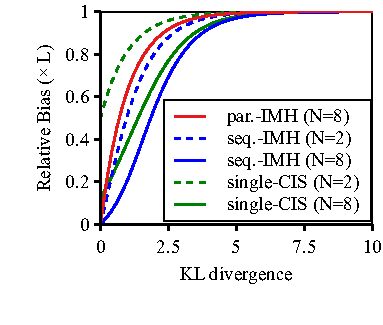
\includegraphics[scale=0.9]{figures/bias_01.pdf}
%%   \vspace{-0.35in}
%%   \caption{Relative bias of different estimators.
%%   For simplicity, we take \(w^* = \exp\left( \DKL{p}{q} \right)\).}\label{fig:bias}
%% \vspace{-0.1in}
%% \end{figure}
%
%% Since \(C_1\left(\vlambda\right) \rightarrow 0\) as \(\norm{\E{\vs\left(\vz; \vlambda\right)}} \rightarrow 0\), the bounds become tighter as SGD converges.
%% Furthermore, at the optimum, the bounds are deterministic regardless of \(\delta\).

%% \vspace{-0.05in}
%% \paragraph{Reducing Bias by Increasing \(N\)}
%% For the seq.-IMH estimator and single-CIS estimator, increasing \(N\) improves the bias decrease rate.
%% However, the bounds depend on \(w^*\), which is bounded below exponentially, as shown by the following proposition.
%% %
%% \begin{theoremEnd}{proposition}\label{thm:kl_bound}
%%   \(w^* = \sup_{\vz} \nicefrac{p\left(\vz\mid\vx\right)}{q_{\vlambda}\left(\vz\right)} \) is bounded below exponentially by the KL divergence such that
%%   \[
%%   \exp\left(\DKL{p\left(\cdot\mid\vx\right)}{ q_{\vlambda}\left(\cdot\right) }\right) \leq w^*.
%%   \]
%% \end{theoremEnd}
%% \vspace{-0.1in}
%% \begin{proofEnd}
%%   \begin{align*}
%%     &\DKL{p\left(\cdot\mid\vx\right)}{ q_{\vlambda}\left(\cdot\right) } \\
%%     &= \int p\left(\vz\mid\vx\right) \log \frac{p\left(\vz\mid\vx\right)}{q_{\vlambda}\left(\vz\right)}\,d\vz \\
%%     &\leq \int p\left(\vz\mid\vx\right) \log w^* \, d\vz \\
%%     &= \log w^*
%%   \end{align*}
%% \end{proofEnd}

%% Thus, in the initial steps of SGD, where the KL divergence is considerable, the bias will also be significant regardless of \(N\).
%% Therefore, increasing \(N\) will not bring a significant reduction in bias.
%% Also, since SGD achieves blinear convergence at best, under practical conditions, bias will be equally high on the the considered methods.
%% To illustrate this point, we visualized the bounds in~\cref{fig:bias}.

%% 
\begin{theoremEnd}{theorem}
  For a parallel state estimator with an IMH kernel, the bias is bounded as
  \[
  \mathrm{Bias}\left[ \vg_{\text{par.-IMH}} \right] \leq 
  C \, \sqrt{
    \chi^2\left( \pi \parallel q \right)
    +
    {\left(
      1 - \frac{1}{w^*}
      \right)}^2
  }
  \]
  where \(C = \Esub{p\left(\vz\mid\vx\right)}{\vs^2\left(\vz\right)}\), \(\chi^2\left(\pi \parallel q \right)\) is the Neyman Chi-square divergence, and \(w^* = \sup_{\vz} \nicefrac{\pi\left(\vz\right)}{q\left(\vz\right)} \).
\end{theoremEnd}
\begin{proofEnd}
  Let us denote \(\pi\left(\vz\right) = p\left(\vz\mid\vx\right)\) for conciseness.
  \begin{align}
    &\norm{
      \int K\left(\vz, \vz^*\right) \vs\left(\vz^*\right) d\vz^*
      - \int \pi\left(\vz\right) \vs\left(\vz\right) d\vz 
    }
    \\
    &=
    \norm{
      \int K\left(\vz, \vz^*\right) \vs\left(\vz^*\right) 
      - \pi\left(\vz^*\right) \vs\left(\vz^*\right) d\vz^*,
    }
    &\text{(\cref{thm:mh_ratio})}
    \\
    &=
    \norm{
      \int \pi\left(\vz^*\right) \min\left(\frac{1}{w\left(\vz\right)}, \frac{1}{w\left(\vz^*\right)}\right)  \vs\left(\vz^*\right) 
      - \pi\left(\vz^*\right) \vs\left(\vz^*\right) d\vz^*
    }
    \\
    &=
    \norm{
      \int \pi\left(\vz^*\right) \vs\left(\vz^*\right)
      \left(
      \min\left(\frac{1}{w\left(\vz\right)}, \frac{1}{w\left(\vz^*\right)}\right)  - 1  
      \right)
      d\vz^*
    }
    \\
    &=
    \sqrt{
      \Esub{\pi}{\vs^2}
    }
    \sqrt{
      \int \pi\left(\vz^*\right)
      {\left(
      \min\left(\frac{1}{w\left(\vz\right)}, \frac{1}{w\left(\vz^*\right)}\right)  - 1  
      \right)}^2
      d\vz^*.
    }
    &\text{(Cauchy-Schwarz)}
    \\
    \intertext{
     Now, let us denote \(A = \{\, \vz^* \mid w\left(\vz^*\right) > w\left(\vz\right) \,\}\).
     Then,
    }
    &=
    \sqrt{
      \Esub{\pi}{\vs^2}
    }
    \sqrt{
      \int_{A^c} \pi\left(\vz^*\right)
      {\left(
      \frac{1}{w\left(\vz^*\right)}  - 1  
      \right)}^2
      d\vz^*
      +
      \int_{A} \pi\left(\vz^*\right)
      {\left(
      \frac{1}{w\left(\vz\right)}  - 1  
      \right)}^2
      d\vz^*
    } \\
    &=
    \sqrt{
      \Esub{\pi}{\vs^2}
    }
    \sqrt{
      \int_{A^c} \pi\left(\vz^*\right)
      {\left(
      \frac{1}{w\left(\vz^*\right)}  - 1  
      \right)}^2
      d\vz^*
      +
      {\left(
      \frac{1}{w\left(\vz\right)}  - 1  
      \right)}^2
      \int_{A} \pi\left(\vz^*\right)
      d\vz^*
    }
    \\
    &\leq
    \sqrt{
      \Esub{\pi}{\vs^2}
    }
    \sqrt{
      \int_{A^c} \pi\left(\vz^*\right)
      {\left(
      \frac{1}{w\left(\vz^*\right)}  - 1  
      \right)}^2
      d\vz^*
      +
      {\left(
      \frac{1}{w\left(\vz\right)}  - 1  
      \right)}^2
    }
    \\
    &\leq
    \sqrt{
      \Esub{\pi}{\vs^2}
    }
    \sqrt{
      \int \pi\left(\vz^*\right)
      {\left(
      \frac{1}{w\left(\vz^*\right)}  - 1  
      \right)}^2
      d\vz^*
      +
      {\left(
      \frac{1}{w\left(\vz\right)}  - 1  
      \right)}^2
    }
    \\
    &=
    \sqrt{
      \Esub{\pi}{\vs^2}
    }
    \sqrt{
      \int \pi\left(\vz^*\right)
      {\left(
      \frac{q\left(\vz^*\right)}{\pi\left(\vz^*\right)}  - 1  
      \right)}^2
      d\vz^*
      +
      {\left(
      \frac{1}{w\left(\vz\right)}  - 1  
      \right)}^2
    }
    \\
    &\leq
    \sqrt{
      \Esub{\pi}{\vs^2}
    }
    \sqrt{
      \int \pi\left(\vz^*\right)
      {\left(
      \frac{q\left(\vz^*\right)}{\pi\left(\vz^*\right)}  - 1  
      \right)}^2
      d\vz^*
      +
      {\left(
      \frac{1}{w^*}  - 1  
      \right)}^2
    },
    \\
    \intertext{
      and finally, by the definition of the Neyman Chi-square divergence,
    }
    &=
    \sqrt{
      \Esub{\pi}{\vs^2}
    }
    \sqrt{
      \chi^2\left( \pi \parallel q \right)
      +
      {\left(
        1 - \frac{1}{w^*}
      \right)}^2
    }.
  \end{align}

  Lastly, for an arbitrary distribution \(\eta\left(\vz\right)\), 
  \begin{align}
    &\norm{
      \int \int \frac{1}{N} \sum^N_{i=1} \eta\left(\vz^{(i)}\right) K\left(\vz^{(i)}, \vz^*\right) \vs\left(\vz^*\right) \, d\vz^{(1:N)} \, d\vz^* - \Esub{\pi}{\vs}
    }
    &\text{(Independence of the chains)}
    \\
    &=
    \norm{
      \int \int \eta\left(\vz\right) K\left(\vz, \vz^*\right) \vs\left(\vz^*\right) d\vz \, d\vz^* - \Esub{\pi}{\vs}
    }
    &\text{(\cref{thm:kernel_apply_bias})}
    \\
    &\leq
    \sqrt{
      \Esub{\pi}{\vs^2}
    }
    \sqrt{
      \chi^2\left( \pi \parallel q \right)
      +
      {\left(
        1 - \frac{1}{w^*}
      \right)}^2
    }.
  \end{align}
\end{proofEnd}


%%% Local Variables:
%%% TeX-master: "master"
%%% End:


%Assuming stationarity, the variance of the sequential state estimator is given as
%
%\vspace{0.05in}
%% {
%% \begin{align}
%%   &\V{\vg_{\text{seq.}}\left(\vlambda\right)} \nonumber\\
%%   &= \frac{\sigma^2}{N} + \frac{2}{N^2} \sum_{i < j}^N \Esub{p\left(\vz_T \mid \vx \right)}{ \Cov{ \vs\left(\vz_{i};\vlambda\right), \vs\left(\vz_{j};\vlambda\right) \mid \vz_{T} } }\label{eq:var_seq}.
%% \end{align}
%% }
%
\textit{Detailed derivation of \textbf{\cref{eq:var_seq}}}

First, remember that the estimator is defined as
  \begin{align*}
    \vg_{\text{seq.}}\left(\vlambda\right) = \frac{1}{N} \sum_{i=1}^N \vs\left(\vlambda; \vz_{T+i}\right),
  \end{align*}
where \( \vz_{T+i} \sim K_{\vlambda_{t-1}}^i\left( \vz_{T}, \cdot \right) \) and \(\vz_T\) is the last Markov-chain state at the previous SGD iteration \(t-1\).
Then, the variance is given as

\begin{align*}
  \V{g_{\text{seq.}}}
  &= \V{ \Esub{K\left(\vz_{T}, \vz\right)}{ \frac{1}{N} \sum_{i=1}^N \vs\left(\vlambda; \vz_{T+i}\right)  \,\Bigg\vert\, \vz_T } }
  + \E{ \Vsub{K\left(\vz_{T}, \vz\right)}{ \frac{1}{N} \sum_{i=1}^N \vs\left(\vlambda; \vz_{T+i}\right) \,\Bigg\vert\,  \vz_T } } &\text{(Total Variance)}  \\
  &= \frac{1}{N^2} \sum_{i=1}^N \Vsub{K\left(\vz_{T}, \vz\right)}{ \E{  \vs\left(\vlambda; \vz_{T+i}\right) \mid \vz_T } }  \\
  &\qquad + \E{ \frac{1}{N^2}  \sum_{i=1}^N  \Vsub{K\left(\vz_{T}, \vz\right)}{ \vs\left(\vlambda; \vz_{T+i}\right)  \mid  \vz_T } 
+ \frac{2}{N^2}  \sum_{i < j}^N \Cov{ s\left(\vlambda; \vz_{T+i}\right), \vs\left(\vlambda; \vz_{T+j}\right) \mid  \vz_T }
  }  \\
  &= \frac{1}{N^2} \sum_{i=1}^N \Vsub{K\left(\vz_{T}, \vz\right)}{ \E{  \vs\left(\vlambda; \vz_{T+i}\right) \mid \vz_T } }  \\
   &\qquad+ \frac{1}{N^2} \sum_{i=1}^N   \Esub{K\left(\vz_{T}, \vz\right)}{ \V{ \vs\left(\vlambda; \vz_{T+i}\right)  \mid  \vz_T } } 
   + \frac{2}{N^2}  \sum_{i < j}^N \E{ \Cov{ \vs\left(\vlambda; \vz_{T+i}\right), \vs\left(\vlambda; \vz_{T+j}\right) \mid  \vz_T }
  },
\intertext{\text{where by assuming stationarity such that \(\vz_{T} \sim p\left(\vz \mid \vx \right)\),}}
  &= \frac{1}{N^2} \sum_{i=1}^N \Vsub{p\left(\vz_T \mid \vx \right)}{ \E{  \vs\left(\vlambda; \vz_{T+i}\right) \mid \vz_T } } 
   \qquad+ \frac{1}{N^2} \sum_{i=1}^N   \Esub{p\left(\vz_T \mid \vx \right)}{ \V{ \vs\left(\vlambda; \vz_{T+i}\right)  \mid  \vz_T } } \\
 &\qquad+ \frac{2}{N^2}  \sum_{i < j}^N \E{ \Cov{ \vs\left(\vlambda; \vz_{T+i}\right), \vs\left(\vlambda; \vz_{T+j}\right) \mid  \vz_T }
  } \\
  &= \frac{1}{N^2} \sum_{i=1}^N \Vsub{p\left(\vz \mid \vx \right)}{ \vs\left(\vlambda; \vz\right) } 
 + \frac{2}{N^2}  \sum_{i < j}^N \E{ \Cov{ \vs\left(\vlambda; \vz_{T+i}\right), \vs\left(\vlambda; \vz_{T+j}\right) \mid  \vz_T }
  }&\text{(Total Variance)} \\
  &= \frac{1}{N} \Vsub{p\left(\vz \mid \vx \right)}{ \vs\left(\vlambda; \vz\right) } 
 + \frac{2}{N^2}  \sum_{i < j}^N \E{ \Cov{ \vs\left(\vlambda; \vz_{T+i}\right), \vs\left(\vlambda; \vz_{T+j}\right) \mid  \vz_T }
  } \\
  &= \frac{\sigma^2}{N}
 + \frac{2}{N^2}  \sum_{i < j}^N \E{ \Cov{ \vs\left(\vlambda; \vz_{T+i}\right), \vs\left(\vlambda; \vz_{T+j}\right) \mid  \vz_T }
  }
\end{align*}

%%% Local Variables:
%%% TeX-master: "master"
%%% End:

%

%% \paragraph{SGD with Biased Gradients}
%% Score climbing with SGD is different from the general SGD setting as it uses biased gradients.
%% One important aspect that 


%
%
\begin{theoremEnd}[]{proposition}\label{thm:imh_bound}
  The rejection rate \(r\,(\vz_{t-1})\) of the IMH sampler is bounded below such that
  \[
  %r(\vz_{t-1}) \geq \frac{1}{1 + N\frac{q_{\vlambda}(\vz_{t-1})}{p(\vz_{t-1}\mid\vx)}}.
  r\,(\vz_{t-1}) \geq 1 - \nicefrac{Z}{w\,(\vz_{t-1})} 
  \]
  where \(Z=\int p\,(\vz,\vx) \, d\vz\) is the normalizing constant.
\end{theoremEnd}
\begin{proofEnd}
  The rejection rate \(r(\vz_{t-1})\) is given as
  \begin{align}
    r\,(\vz_{t-1}) = 1 - \int \alpha\left(\vz, \vz_{t-1} \right) \, q_{\vlambda}(\vz) \, d\vz.
  \end{align}
  For an IMH sampler with the Metropolis-Hastings acceptance function and independent proposals, the rejection rate is bounded such that
  \begin{align}
    r\,(\vz_{t-1})
    &= 1 - \int \min\left(\frac{w\,(\vz)}{w\,(\vz_{t-1})}, 1 \right) \, q_{\vlambda}(\vz)\,d\vz \\
    &= 1 - \frac{1}{w\,(\vz_{t-1})} \int \min\Big(w\,(\vz), w\,(\vz_{t-1})\Big) \, q_{\vlambda}(\vz)\,d\vz \\
    &= 1 - \frac{1}{w\,(\vz_{t-1})} \int \min\left(\frac{p\,(\vz,\vx)}{q_{\vlambda}(\vz)}, w\,(\vz_{t-1})\right) \, q_{\vlambda}(\vz)\,d\vz \\
    &=    1 - \frac{1}{w\,(\vz_{t-1})} \int \min\Big(p\,(\vz,\vx), w\,(\vz_{t-1})\,q_{\vlambda}(\vz)\Big) \, d\vz  \\
    &\geq 1 - \frac{1}{w\,(\vz_{t-1})} \int p\,(\vz,\vx) \, d\vz \label{eq:imh_min_comp} \\
    &=    1 - \frac{Z}{w\,(\vz_{t-1})} 
  \end{align}
  The inequality in Equation~\eqref{eq:imh_min_comp} follows from \(\min\big(p\,(\vz,\vx), w\,(\vz_{t-1})\,q_{\vlambda}(\vz)\big) \leq p\,(\vz,\vx) \) for \(\forall \vz \in \mathcal{Z}\).
\end{proofEnd}

%%% Local Variables:
%%% TeX-master: "master"
%%% End:

%

%
\begin{theoremEnd}{proposition}\label{thm:approx_var}
  Assuming \(w\,(\vz_{t-1})\) is large enough to make \(r\,(\vz\mid\vz^{(1:N)})\) independent of \(\vz^{(1:N)}\), the variance can be approximated by
  \begin{align}
    \Vsub{q_{\vlambda}}{ \E{ f \mid \vz_{t-1}, \vz^{(1:N)} } } \approx {\big(1 - r\,(\vz_{t-1})\big)}^2\,\Vsub{q_{\vlambda}}{ f_{\text{IS}} \,\middle\vert\, \vz_{t-1} }.
  \end{align}
\end{theoremEnd}
\begin{proofEnd}
  We evaluate the variance by approximating the rejection probability as an independent constant.
  First,
  \begin{align}
    &\Vsub{q_{\vlambda}}{ \E{ f \mid \vz_{t-1}, \vz^{(1:N)} } }. \\
    \intertext{
      Applying~\eqref{eq:cis_kernel_inter},
    }
    &= \Vsub{q_{\vlambda}}{ \big(1 - r\,(\vz_{t-1}\mid\vz^{(1:N)})\big)\, f_{\mathrm{IS}}
      + r\,(\vz_{t-1}\mid\vz^{(1:N)})\,f(\vz_{t-1}) \;\middle\vert\; \vz_{t-1}} \\
    &\approx \Vsub{q_{\vlambda}}{ \big(1 - r\,(\vz_{t-1})\big)\, f_{\mathrm{IS}}
      + r\,(\vz_{t-1})\,f(\vz_{t-1}) \;\middle\vert\; \vz_{t-1}} \\
    &= \Vsub{q_{\vlambda}}{ \big(1 - r\,(\vz_{t-1})\big)\, f_{\mathrm{IS}} \;\middle\vert\; \vz_{t-1} } \label{eq:approx_var_constant} \\
    &= {\big(1 - r\,(\vz_{t-1})\big)}^2 \, \Vsub{q_{\vlambda}}{ f_{\mathrm{IS}} \;\middle\vert\; \vz_{t-1} }. \label{eq:approx_var_linear} 
  \end{align}
  The equality of~\eqref{eq:approx_var_constant} follows from the fact that \(r\,(\vz_{t-1})\,f(\vz_{t-1})\) is a constant.
\end{proofEnd}

%%% Local Variables:
%%% TeX-master: "master"
%%% End:


%%% Local Variables:
%%% TeX-master: "master"
%%% End:
